% (c)~2014 Claudio Carboncini - claudio.carboncini@gmail.com
% (c)~2014 Dimitrios Vrettos - d.vrettos@gmail.com
% (c) 2015 Daniele Zambelli daniele.zambelli@gmail.com

\subsection{Esercizi dei singoli paragrafi}

% \subsubsection*{\numnameref{sec:01_}}

% \begin{esercizio}
% \label{ese:D.1}
% testo esercizio
% \end{esercizio}
% 
% \begin{esercizio}\label{ese:03.1}
% Consegna:
%  \begin{enumeratea}
%   \item  
%  \end{enumeratea}
% \end{esercizio}
% 
% \subsection{Esercizi riepilogativi}
% 
% \begin{esercizio}
% \label{ese:D.2}
% testo esercizio
% \end{esercizio}
% 
% \begin{esercizio}\label{ese:03.2}
% Consegna:
%  \begin{enumeratea}
%   \item  
%  \end{enumeratea}
% \end{esercizio}

\begin{esercizio}[\Ast]
 \label{ese:3.1}
Risolvi le seguenti equazioni di secondo grado pure.
\begin{multicols}{2}
 \begin{enumeratea}
 \item~$x^{2}-1 = 0$ \hfill$\left[...\right]$
 \item~$x^{2}=\dfrac{49}{25}$ \hfill$\left[...\right]$
 \item~$2x^{2} - 32 = 0$ \hfill$\left[x_{1}=+4 \vee x_{2}=-4\right]$
 \item~$x^{2}-25=0$ \hfill$\left[...\right]$
 \item~$16 x^{2}=1$ \hfill$\left[...\right]$
 \item~$3x^{2}+3=0$ \hfill$\left[\emptyset\right]$
 \item~$x^{2}-9=0$ \hfill$\left[...\right]$
 \item~$25=9 x^{2}$ \hfill$\left[...\right]$
 \item~$x^{2} - 3 = 0$ \hfill$\left[x_{1} = \sqrt{3} \vee x _{2} = - 
\sqrt{3}\right]$
 \item~$x^{2} + 36 = 0$ \hfill$\left[...\right]$
 \item~$4 - x^{2} = 0$ \hfill$\left[...\right]$
 \item~$x^{2} + 4 = 0$ \hfill$\left[\emptyset\right]$
 \item~$x^{2} = 49$ \hfill$\left[...\right]$
 \item~$4 - 9 x^{2} = 0$ \hfill$\left[...\right]$
 \item~$5 x^{2} - 3 = 0$ \hfill$\left[x_{1,2} = \dfrac{\pm 
\sqrt{15}}{5}\right]$
 \item~$4 x^{2} - 9 = 0$ \hfill$\left[...\right]$
 \item~$9 x^{2} - 25 = 0$ \hfill$\left[...\right]$
 \item~$6 x^{2} = 0$ \hfill$\left[x_{1,2} = 0\right]$
 \item~$2 x^{2} - 1 = 0$ \hfill$\left[...\right]$
 \item~$4 x^{2} + 16 = 0$ \hfill$\left[...\right]$
 \item~$1 + x^{2} = 50$ \hfill$\left[x_{1,2} = \pm 7\right]$
 \item~$3 x^{2} - 1 = 0$ \hfill$\left[...\right]$
 \item~$27 x^{2} - 3 = 0$ \hfill$\left[...\right]$
 \item~$7 x^{2} = 28$ \hfill$\left[x_{1,2} = \pm 2\right]$
 \end{enumeratea}
 \end{multicols}
\end{esercizio}

% \begin{esercizio}[\Ast]
%  \label{ese:3.3}
% Risolvi le seguenti equazioni di secondo grado pure.
% \begin{multicols}{3}
%  \begin{enumeratea}
%  \item~$4 x^{2} - 4 = 0$ \hfill$\left[...\right]$
%  \item~$5 x^{2} - 125 = 0$ \hfill$\left[...\right]$
%  \item~$0,04 x^{2} = 1$ \hfill$\left[x_{1,2} = \pm 5\right]$
%  \item~$x^{2} - 0,01 = 0$ \hfill$\left[...\right]$
%  \item~$0,5 x^{2} - 4,5 = 0$ \hfill$\left[...\right]$
%  \item~$0,09 x^{2} = 0,01$ \hfill$\left[x_{1,2} = \pm \dfrac{1}{3}\right]$
%  \item~$\dfrac{1}{2} x^{2} - 2 = 0$ \hfill$\left[...\right]$
%  \item~$x^{2} - \dfrac{9}{4} = 0$ \hfill$\left[...\right]$
%  \item~$x^{2} - \dfrac{1}{6} = 0$ \hfill$\left[...\right]$
%  \item~$121 x^{2} - \dfrac{1}{169} = 0$ 
%   \hfill$\left[x_{1,2} = \pm \dfrac{\sqrt{6}}{6}\right]$
%  \item~$x^{2} + \dfrac{9}{4} = 0$ \hfill$\left[...\right]$
%  \item~$4 \left(x^{2}-\dfrac{3}{4}\right)= 13$ 
%   \hfill$\left[x_{1,2} = \pm 2\right]$
%  \end{enumeratea}
%  \end{multicols}
% \end{esercizio}

% \begin{esercizio}[\Ast]
%  \label{ese:3.4}
% Risolvi le seguenti equazioni di secondo grado pure.
% \begin{multicols}{2}
%  \begin{enumeratea}
%  \item~$x^{2} - \sqrt{3} = 0$ \hfill$\left[...\right]$
%  \item~$- 9 x^{2} = - 1$ \hfill$\left[...\right]$
%  \item~$4 x^{2} = - 9$ \hfill$\left[\emptyset\right]$
%  \item~$x^{2} + 6 = 42$ \hfill$\left[...\right]$
%  \item~$5 - 125 x^{2} = 0$ \hfill$\left[...\right]$
%  \item~$18 - x^{2} = 0$ \hfill$\left[x_{1,2} = \pm 3 \sqrt{2}\right]$
%  \item~$(x + 3)^{2} = 6 x + 34$ \hfill$\left[...\right]$
%  \item~$(x + 1)^{2} = 25$ \hfill$\left[...\right]$
%  \item~$(x - \sqrt{3}) (x + \sqrt{3}) = 13$ 
%   \hfill$\left[x_{1,2} = \pm \sqrt{10}\right]$
%  \item~$(x + \sqrt{2})^{2} = 2 \sqrt{2} x$ \hfill$\left[...\right]$
%  \item~$(x - 2)^{2} + (1 - x)^{2} = 1 - 6x$ \hfill$\left[...\right]$
%  \item~$(\sqrt{2} x - \sqrt{3}) (\sqrt{2} x + \sqrt{3}) = 0$ 
%   \hfill$\left[x_{1,2} = \pm \dfrac{\sqrt{6}}{2}\right]$
%  \end{enumeratea}
%  \end{multicols}
% \end{esercizio}

\begin{esercizio}[\Ast]
\label{ese:3.5}
Risolvi le seguenti equazioni di secondo grado spurie.
\begin{multicols}{2}
 \begin{enumeratea}
 \item~$x^{2} - 3 x = 0$ \hfill$\left[...\right]$
 \item~$3 x^{2} - 2 x = 0$ 
  \hfill$\left[x_{1} = 0 \vee x_{2} = \dfrac{2}{3}\right]$
 \item~$7 x^{2} + 2 x = 0$ 
  \hfill$\left[x_{1} = 0 \vee x_{2} = - \dfrac{2}{7}\right]$
 \item~$x^{2} + 2 x = 0$ \hfill$\left[...\right]$
 \item~$x^{2} + 5 x = 0$ 
  \hfill$\left[x_{1} = 0 \vee x_{2} = - 5\right]$
 \item~$x^{2} - x = 0$ \hfill$\left[...\right]$
 \item~$18 x^{2} - 36 x = 0$ \hfill$\left[x_{1} = 0 \vee x_{2} = 2\right]$
 \item~$2x^{2} + 6x = 0$ \hfill$\left[...\right]$
 \item~$1000 x - 2000 x^{2} = 0$ \hfill$\left[x_{1} = 0 \vee x_{2} = 
\dfrac{1}{2}\right]$
 \item~$9x^{2} + 16x = 0$ \hfill$\left[...\right]$
 \item~$6 x^{2} = 5 x$ \hfill$\left[x_{1} = 0 \vee x_{2} = 
\dfrac{5}{6}\right]$
 \item~$5x = 25x^{2}$ \hfill$\left[...\right]$
 \item~$3 x^{2} - 2 x = 4 x$ \hfill$\left[x_{1} = 0 \vee x_{2} = 2\right]$
 \item~$81x^{2} = 9x$ \hfill$\left[...\right]$
 \item~$0,1 x^{2} - 0,5 x = 0$ \hfill$\left[x_{1} = 0 \vee x_{2} = 5\right]$
 \item~$7x^{2} - 2x = 0$ \hfill$\left[...\right]$
 \item~$0,5 x^{2} + 0,1 x = 0$ \hfill$\left[x_{1} = 0 \vee x_{2} = - 
0,2\right]$
 \item~$x^{2} + \dfrac{1}{2} x = 0$ \hfill$\left[...\right]$
 \item~$\dfrac{11}{3} x^{2} = - 2 x$ 
  \hfill$\left[x_{1} = 0 \vee x_{2} = - \dfrac{6}{11}\right]$
 \item~$\dfrac{1}{2} ( x - 2 )^{2} - x = 2$
  \hfill$\left[x_{1} = 0 \vee x_{2} = 6\right]$
%  \item~$(x - 1) (x + 3) = 3 x^{2} - 3$
%   \hfill$\left[x_{1} = 0 \vee x_{2} = 1\right]$
 \item~$x^{2} + \sqrt{2} x = 0$ 
  \hfill$\left[x_{1} = 0 \vee x_{2} = - \sqrt{2}\right]$
 \item~$\dfrac{1}{2} x - \dfrac{1}{4} x^{2} = 0$ 
  \hfill$\left[x_{1} = 0 \vee x_{2} = 2\right]$
 \item~$(3 x - 2)^{2} - 4 = 6 x^{2}$
  \hfill$\left[x_{1} = 0 \vee x_{2} = 4\right]$
 \item~$5 \sqrt{2} x^{2} - 2 \sqrt{2} x = 0$ 
  \hfill$\left[x_{1} = 0 \vee x_{2} = \dfrac{2}{5}\right]$
 \end{enumeratea}
 \end{multicols}
\end{esercizio}

% \begin{esercizio}[\Ast]
%  \label{ese:3.8}
% Risolvi le seguenti equazioni di secondo grado spurie.
% \begin{multicols}{3}
%  \begin{enumeratea}
%  \item~$\sqrt{2} x^{2} + \sqrt{3} x = 0$ \hfill$\left[...\right]$
%  \item~$- 2x^{2} + 4x = 0$ \hfill$\left[...\right]$
%  \item~$\dfrac{1}{6} x^{2} + \dfrac{1}{4} x = 0$ \hfill$\left[...\right]$
%  \end{enumeratea}
%  \end{multicols}
% \end{esercizio}
% 
% \begin{esercizio}[\Ast]
%  \label{ese:3.9}
% Risolvi le seguenti equazioni di secondo grado spurie.
% \begin{multicols}{3}
%  \begin{enumeratea}
%  \item~$3x^{2} - \dfrac{4}{3} x = 0$ 
%   \hfill$\left[x_{1} = 0 \vee x_{2} = \dfrac{4}{9}\right]$
%  \item~$(x - 2)^{2} = 4$ \hfill$\left[...\right]$
%  \item~$(x + 1)^{2} = 1$ 
%   \hfill$\left[x_{1} = 0 \vee x_{2} = - 2\right]$
%  \item~$(x + \sqrt{2})^{2} = 2$ \hfill$\left[...\right]$
%  \item~$77 x - 11 x^{2} = 0$ 
%   \hfill$\left[x_{1} = 0 \vee x_{2} = 7\right]$
%  \item~$\dfrac{3}{4} x^{2} - \dfrac{3}{2} x = 0$ \hfill$\left[...\right]$
%  \end{enumeratea}
%  \end{multicols}
% \end{esercizio}
% % 
% \begin{esercizio}[\Ast]
%  \label{ese:3.11}
% Risolvi le seguenti equazioni di secondo grado spurie.
%  \begin{enumeratea}
%  \item~$(x - 2)^{2} + (1 - x)^{2} = 5$
%   \hfill$\left[...\right]$
%  \item~$(x -2)^{3} -4 (2 x -1) = (x +2) \left(x^{2} -2 x +4\right) -12$
%   \hfill$\left[...\right]$
%  \item~$(\sqrt{2} + x)^{3} - (\sqrt{3} + x)^{3} = 2 \sqrt{2} - 3\sqrt{3}$
%   \hfill$\left[x_{1} = 0 \vee x_{2} = - (\sqrt{2} + \sqrt{5})\right]$
%  \item~$(\sqrt{2} x - \sqrt{3}) (\sqrt{2} x + \sqrt{3}) + (\sqrt{3} x + 
% \sqrt{3})^{2} + (x - 1)^{2} = 1$
%   \hfill$\left[...\right]$
%  \item~$\left(x^{2} + \sqrt{2} \right) (\sqrt{3} - 1) + (2 x +\sqrt{3}) 
% (\sqrt{2} - 1) - \sqrt{2} + \sqrt{3} = 0$
%   \hfill$\left[...\right]$
%  \end{enumeratea}
% \end{esercizio}

% \subsection*{3.2 - Risoluzione di un'equazione completa}
\numnameref{sec:eq2gr_completa}

\begin{esercizio}[\Ast]
 \label{ese:3.12}
Risolvi le seguenti equazioni di secondo grado complete.
\begin{multicols}{2}
 \begin{enumeratea}
 \item~$x^{2}-5 x + 6=0$
  \hfill$\left[x_{1} = 2 \vee x_{2} = 3\right]$
 \item~$x^{2} + x-20=0$
  \hfill$\left[x_{1} =-5 \vee x_{2} = 4\right]$
 \item~$2 x^{2}-6 x-6=0$
  \hfill$\left[x_{1,2} = \dfrac{3 \pm \sqrt{21}}{2}\right]$
 \item~$x^{2}-3 x + 6=0$
  \hfill$\left[\emptyset\right]$
 \item~$- x^{2} + x + 42=0$
  \hfill$\left[x_{1} =-6 \vee x_{2} = 7\right]$
 \item~$- x^{2} + 10 x-25=0$
  \hfill$\left[x_{1} = x_{2} = 5\right]$
 \item~$- 2 x^{2} + 7 x-5=0$
  \hfill$\left[x_{1} = 1 \vee x_{2} = \dfrac{5}{2}\right]$
 \item~$3 x^{2} + 2 x-1=0$
  \hfill$\left[x_{1} =-1 \vee x_{2} = \dfrac{1}{3}\right]$
 \item~$x^{2}-4 x + 9 = 0$
  \hfill$\left[\emptyset\right]$
 \item~$x^{2}-4 x-9 = 0$
  \hfill$\left[x_{1,2} = 2 \pm \sqrt{13}\right]$
 \item~$2 x^{2}-\sqrt{5} x-1 = 0$
  \hfill$\left[x_{1,2} = \dfrac{\sqrt{5} \pm \sqrt{13}}{4}\right]$
 \item~$x^{2}-3 x-2=0$
  \hfill$\left[x_{1,2} = \dfrac{3 \pm \sqrt{17}}{2}\right]$
 \item~$x^{2}-5 x + 3 = 0$
  \hfill$\left[x_{1,2} = \dfrac{5 \pm \sqrt{13}}{2}\right]$
 \item~$x^{2}-2 \sqrt{3} x-4=0$
  \hfill$\left[x_{1,2} = \sqrt{3} \pm \sqrt{7}\right]$
 \item~$x^{2} + 6 x-2 = 0$
  \hfill$\left[x_{1,2} =-3 \pm \sqrt{11}\right]$
 \item~$- x^{2} + 4 x-7=0$
  \hfill$\left[\emptyset\right]$
%  \item~$2 x^{2}-\sqrt{5} x-1=0$
%   \hfill$\left[x_{1} =-\sqrt{2} \vee x_{2} = \dfrac{3 \sqrt{2}}{2}\right]$
 \item~$- \dfrac{4}{3} x^{2}-x + \dfrac{3}{2}=0$
  \hfill$\left[x_{1} =-\dfrac{3}{2} \vee x_{2} = \dfrac{3}{4}\right]$
 \item~$- \dfrac{4}{5} x^{2} + \dfrac{1}{2} x-\dfrac{1}{20}=0$
  \hfill$\left[x_{1} = \dfrac{1}{8} \vee x_{2} = \dfrac{1}{2}\right]$
%  \item~$x^{2}-\sqrt{5} x-\sqrt{5}=0$
%   \hfill$\left[x_{1,2} = \dfrac{\sqrt{5} \pm \sqrt{5 + 4 
% \sqrt{5}}}{2}\right]$
%  \item~$x^{2} + (\sqrt{2}-\sqrt{3}) x-\sqrt{6} = 0$
%   \hfill$\left[x_{1} =-\sqrt{2} \vee x_{2} = \sqrt{3}\right]$
 \item~$(x-2) (3-2 x) = x-2$
  \hfill$\left[x_{1} = 1 \vee x_{2} = 2\right]$
 \end{enumeratea}
 \end{multicols}
\end{esercizio}

\begin{esercizio}[\Ast]
 \label{ese:3.17}
Risolvi le seguenti equazioni di secondo grado complete.
\begin{multicols}{2}
 \begin{enumeratea}
 \item~$(x + 5)^{2} = 5 (4 x + 5)$
  \hfill$\left[x_{1} = 0 \vee x_{2} = 10\right]$
 \item~$x^{2} + 6 x-3 = 0$
  \hfill$\left[x_{1,2} =-3 \pm 2 \sqrt{3}\right]$
 \item~$x^{2}-3 x-\dfrac{5}{2} = 0$
  \hfill$\left[x_{1,2} = \dfrac{3 \pm \sqrt{19}}{2}\right]$
 \item~$2 x^{2}-3 x + 1 = 0$
  \hfill$\left[x_{1} = 1 \vee x_{2} = \dfrac{1}{2}\right]$
 \item~$\dfrac{4}{3} x^{2}-\dfrac{1}{3} x-1 = 0$
  \hfill$\left[x_{1} = 1 \vee x_{2} =-\dfrac{3}{4}\right]$
 \item~$3 x^{2} + x-2 = 0$
  \hfill$\left[x_{1} =-1 \vee x_{2} = \dfrac{2}{3}\right]$
 \item~$3 x^{2}-\dfrac{2}{3} x-1 = 0$
  \hfill$\left[x_{1,2} = \dfrac{1 \pm 2 \sqrt{7}}{9}\right]$
%  \item~$\sqrt{2} x^{2}-x-3 \sqrt{2} = 0$
%   \hfill$\left[x_{1} =-\sqrt{2};~x_{2} = \dfrac{3 \sqrt{2}}{2}\right]$
%  \item~$(3 x + 1)^{2}-(2 x + 2)^{2} = 0$
%   \hfill$\left[x_{1} =-\dfrac{3}{5} \vee x_{2} = 1\right]$
%  \item~$(x + 200)^{2} + x + 200 = 2$
%   \hfill$\left[x_{1} =-202 \vee x_{2} =-199\right]$
 \item~$3 x^{2}-2 x-2 = 0$
  \hfill$\left[x_{1,2} = \dfrac{1 \pm \sqrt{7}}{3}\right]$
 \item~$4 x^{2}-8 x + 3 = 0$
  \hfill$\left[x_{1} = \dfrac{1}{2} \vee x_{2} = \dfrac{3}{2}\right]$
%  \item~$x^{2}-(\sqrt{2} + \sqrt{3}) x + \sqrt{6} = 0$
%   \hfill$\left[x_{1} = \sqrt{2} \vee x_{2} = \sqrt{3}\right]$
%  \item~$(x^{2} + x + 1) (x^{2}-x-1) = (x^{2}-1)^{2}$
%   \hfill$\left[x_{1,2} = 1 \pm \sqrt{3}\right]$
%  \item~$7 x^{2}-2 x-5 = 0$
%   \hfill$\left[x_{1} = 1 \vee x_{2} =-\dfrac{5}{7}\right]$
 \end{enumeratea}
 \end{multicols}
\end{esercizio}

\begin{esercizio}[\Ast]
\label{ese:3.21}
Risolvi, applicando quando possibile la formula ridotta o ridottissima.
\begin{multicols}{2}
 \begin{enumeratea}
 \item~$40 x^{2} + 80 x-30 = 0$
  \hfill$\left[x_{1,2} = \dfrac{- 2 \pm \sqrt{7}}{2}\right]$
 \item~$5 x^{2}-4 x + 1 = 0$
  \hfill$\left[\emptyset\right]$
 \item~$5 x^{2}-4 x-9 = 0$
  \hfill$\left[x_{1} =-1 \vee x_{2} = \dfrac{9}{5}\right]$
 \item~$\dfrac{3}{2} x^{2} + 2 x-\dfrac{3}{4} = 0$
  \hfill$\left[x_{1,2} = \dfrac{- 4 \pm \sqrt{34}}{6}\right]$
 \item~$6 x^{2}-4 x-2 = 0$
  \hfill$\left[x_{1} = 1 \vee x_{2} =-\dfrac{1}{3}\right]$
%  \item~$90 x^{2}-180 x-270 = 0$
%   \hfill$\left[x_{1} = 3 \vee x_{2} =-1\right]$
 \item~$\dfrac{3}{2} x^{2}-4 x + 2 = 0$
  \hfill$\left[x_{1} = 2 \vee x_{2} = \dfrac{2}{3}\right]$
 \item~$\dfrac{4}{3} x^{2}-6 x + 6 = 0$
  \hfill$\left[x_{1} = 3 \vee x_{2} = \dfrac{3}{2}\right]$
 \item~$x^{2}-6 x + 1 = 0$
  \hfill$\left[x_{1,2} = 3 \pm 2 \sqrt{2}\right]$
 \item~$3 x^{2}-12 x-3 = 0$
  \hfill$\left[x_{1,2} = 2 \pm \sqrt{5}\right]$
 \item~$7 x^{2}-6 x + 8 = 0$
  \hfill$\left[\emptyset\right]$
 \item~$3 x^{2}-18 x + 27 = 0$
  \hfill$\left[x_{1,2} =3\right]$
 \item~$9 x^{2}-12 x + 4 = 0$
  \hfill$\left[x_{1,2} = \dfrac{2}{3}\right]$
 \item~$4 x^{2}-32 x + 16 = 0$
  \hfill$\left[x_{1,2} = 4 \pm 2 \sqrt{3}\right]$
 \item~$3 x^{2} + 10 x + 20 = 0$
  \hfill$\left[\emptyset\right]$
 \end{enumeratea}
 \end{multicols}
\end{esercizio}

% \subsection*{Altri esercizi sulle equazioni di 2° grado}

\begin{esercizio}[\Ast]
\label{ese:3.25}
Risolvi le seguenti equazioni di secondo grado.
\begin{multicols}{2}
 \begin{enumeratea}
 \item~$3 x-x^{2} = x^{2} + 3 (x-2)$
  \hfill$\left[x_{1,2} = \pm \sqrt{3}\right]$
 \item~$2 (x-1) (x + 1) = 2$
  \hfill$\left[x_{1,2} =\pm \sqrt{2}\right]$
 \item~$(2 x-1) (4-x)-11 x = (1-x)^{2}$
  \hfill$\left[\emptyset\right]$
 \item~$2x^{2} = x + x^{2}-(x + \sqrt{x}) (x-\sqrt{x})$
  \hfill$\left[...\right]$
 \item~$(x-3)^{2} = 9-6 x$
  \hfill$\left[x_{1,2}= 0\right]$
 \item~$\dfrac{3 x-2}{2} = x^{2}-2$
  \hfill$\left[x_{1} = 2 \vee x_{2} =-\dfrac{1}{2}\right]$
 \item~$(2 x-3) (2 x + 3) = 27$
  \hfill$\left[x_{1,2} =\pm 3\right]$
 \item~$\dfrac{x-3}{2}-\dfrac{x^{2} + 2}{3} = 1 + x$
  \hfill$\left[\emptyset\right]$
 \item~$(x-2)^{3}-x^{3} = x^{2}-4$
  \hfill$\left[x_{1,2} = \dfrac{6 \pm 2 \sqrt{2}}{7}\right]$
 \item~$\dfrac{(x-1)^{2}}{2}-\dfrac{2 x-5}{3} =-\dfrac{5}{3} x$
  \hfill$\left[\emptyset\right]$
 \item~$(2-x)^{3}-(2-x)^{2} = \dfrac{3-4 x^{3}}{4}$
  \hfill$\left[\emptyset\right]$
 \end{enumeratea}
 \end{multicols}
\end{esercizio}

\begin{esercizio}[\Ast]
 \label{ese:3.30}
Risolvi le seguenti equazioni di secondo grado.
 \begin{enumeratea}
 \item~$9 x^{2} + 12 x + 1 = 0$
  \hfill$\left[x_{1,2} = \dfrac{- 2 \pm \sqrt{3}}{3}\right]$
 \item~$\dfrac{x-2}{3}-(3 x + 3)^{2} = x$
  \hfill$\left[x_{1} =-1 \vee x_{2} =-\dfrac{29}{27}\right]$
 \item~$(3 x + 1) \left(\dfrac{5}{2} + x \right) = 2 x-1$
  \hfill$\left[x_{1} =-1 \vee x_{2} =-\dfrac{7}{6}\right]$
 \item~$(3 x-2)^{2} + (5 x-1)^{2} = (3 x-2) (5 x-1)$
  \hfill$\left[\emptyset\right]$
 \item~$(x-2)^{3}-1 = x^{3} + 12 x-11$
  \hfill$\left[x_{1,2} = \dfrac{\pm \sqrt{3}}{3}\right]$
 \item~$x (1-5 x) = [ 3-(2 + 5 x) ] x-(x^{2}-1)$
  \hfill$\left[x_{1,2} =\pm 1\right]$
 \item~$(x + 1)^{3}-(x + 2)^{2} = \dfrac{2 x^{3}-1}{2}$
  \hfill$\left[x_{1,2} = \dfrac{1 \pm \sqrt{21}}{4}\right]$
 \item~$(x + 2)^{3} + 4 x^{2} = (x-2)^{3} + 16$
  \hfill$\left[x_{1} = x_{2} = 0\right]$
 \item~$3 \left(x +\sqrt{2} \right)^{2}-18 \left(x +\sqrt{2}\right) +27 = 0$
  \hfill$\left[x_{1,2}= 3-\sqrt{2}\right]$
 \item~$(4-3 x)^{3} + 27 x^{3} = 64 + 24 x$
  \hfill$\left[x_{1} = 0 \vee x_{2} = \dfrac{14}{9}\right]$
 \item~$\left(\dfrac{x-1}{3}-\dfrac{x}{6} \right)^{2} = (x + 1)^{2}$
  \hfill$\left[x_{1} =-\dfrac{8}{5} \vee x_{2} =-\dfrac{4}{7}\right]$
 \item~$(\sqrt{3} x + 1)^{2} + (\sqrt{3} x-1)^{2}-3 (\sqrt{3}x + 1) 
(\sqrt{3} x-1) = 0$
  \hfill$\left[x_{1,2} = \pm \sqrt{\dfrac{5}{3}}\right]$
 \item~$\dfrac{(2 x + 1) (x-2)}{3} + \dfrac{(x + \sqrt{5}) (x -\sqrt{5})}{2} 
= \dfrac{(x-1)^{2}}{6}$
  \hfill$\left[x_{1,2} = \dfrac{1 \pm \sqrt{31}}{3}\right]$
 \item~$\left(\dfrac{1}{2} x +1 \right)^{3} = \left(\dfrac{1}{2} x-1\right) 
\left(\dfrac{1}{2} x + 1 \right)^{2}$
  \hfill$\left[x_{1,2}=-2\right]$
 \item~$\dfrac{(3 x-1)^{2}}{3}-\dfrac{(1-2 x)^{2}}{5} + \dfrac{3 x (x-1)}{5} 
+ \dfrac{(1 + x)^{2}}{3} = 0$
  \hfill$\left[\emptyset\right]$
 \item~$\dfrac{1}{\sqrt{10}} x^{2} + 1 = \left(\dfrac{1}{\sqrt{2}} 
+\dfrac{1}{\sqrt{5}} \right) x$
  \hfill$\left[...\right]$
 \item~$(3 x-1)^{2} + (2 x + 1)^{2} = (3 x-1) (2 x + 1)$
  \hfill$\left[\emptyset\right]$
 \item~$(x + 1)^{4}-(x + 1)^{3} = x^{3} (x + 4)-x (x + 1)^{2} + 3 x$
  \hfill$\left[x_{1} = 0 \vee x_{2} = \dfrac{1}{5}\right]$
 \item~$\left(\dfrac{1}{2} x^{2} + 1 \right)^{3} + \dfrac{1}{6} x^{3} = 
\left(\dfrac{1}{2} x^{2}-1 \right)^{3} + \dfrac{1}{6} (x + 1)^{3} + 
\dfrac{3}{2} x^{4}$
  \hfill$\left[x_{1,2} = \dfrac{- 3 \pm \sqrt{141}}{6}\right]$
 \item~$\dfrac{x-2}{2} \cdot \dfrac{x + 2}{3} + \dfrac{1}{3} 
\left[\dfrac{1}{2}-\left(x + \dfrac{1}{2} \right) \right] + 4 \left(x 
-\dfrac{1}{2} 
\right) \left(x + \dfrac{1}{2} \right) + \dfrac{5}{3} = 0$
  \hfill$\left[x_{1} = 0 \vee x_{2} = \dfrac{2}{25}\right]$
 \item~$(2-3 x)^{2}-1 = 8 (1-2 x) + (2 x + 1)^{2}-1$
  \hfill$\left[x_{1,2} =\pm 1\right]$
 \item~$x^{2} + \left(\sqrt{3}-\sqrt{2} \right) x-\sqrt{6} = 0$
  \hfill$\left[x_{1} =-\sqrt{3} \vee x_{2} = + \sqrt{2}\right]$
%  \item~$\dfrac{2 \sqrt{3} x + 1}{\sqrt{2}}-\left(x-\sqrt{3} \right)^{2} = 
% \dfrac{1-3 \sqrt{2} x}{\sqrt{2}} + \sqrt{3} x \left(\sqrt{2}+ 2 \right)$
%   \hfill$\left[...\right]$
%  \item~$\sqrt{3} (2 x-30)^{2}-2 \sqrt{27} (60-4 x) = 0$
%   \hfill$\left[...\right]$
 \item~$\left(2 x + \dfrac{1}{2} \right)^{2}-\dfrac{1}{2} 
        \left(\dfrac{1}{2} x-1 \right)^{2} + \left(x-\dfrac{1}{2} \right) 
        \left(x + \dfrac{1}{2} \right) = 0$
  \hfill$\left[...\right]$
 \end{enumeratea}
\end{esercizio}

% \begin{esercizio}[\Ast]
%  \label{ese:3.33}
% Risolvi le seguenti equazioni di secondo grado.
%  \begin{enumeratea}
%  \item~$\dfrac{x^{2}-16}{9} + \dfrac{(x-1)^{2}}{3} = \dfrac{x (x -2)}{9} 
% + \left(x-\dfrac{5}{2} \right) \left(x + \dfrac{1}{3}\right)$
%   \hfill$\left[...\right]$
%  \end{enumeratea}
% \end{esercizio}
% 
%  \begin{esercizio}[\Ast]
% \label{ese:3.34}
% Risolvi le seguenti equazioni di secondo grado.
%  \begin{enumeratea}
%  \item~$\dfrac{(x-1) (x + 2)}{2} + \dfrac{(x + 2) (x-3)}{3} =\dfrac{(x-3) 
% (x + 4)}{6}$
%   \hfill$\left[...\right]$
%  \item~$\left(2 x-\dfrac{1}{2} \right)^{2} + \left(\dfrac{x-1}{2} 
% -\dfrac{x}{3} \right) x =-x^{2} + \dfrac{2}{3} 
% \left(x-\dfrac{1}{2}\right) x-\dfrac{1}{2} x + 
% \dfrac{1}{9}$
%   \hfill$\left[...\right]$
%  \item~$\dfrac{1}{4} (2 x-1)^{2}-\dfrac{1}{3} (x-1)^{2} +\dfrac{(x-2) (x 
% + 2)}{2}-\dfrac{1}{6} x + \dfrac{1}{6} = 0$
%   \hfill$\left[...\right]$
%  \item~$\dfrac{1}{2} (2 x-1) (x + 1) + \dfrac{1}{3} \left(x^{2}-5\right) + 
% 2 x (x-1) (x + 1) = 2 (x + 2)^{3}-(2 x-1)^{2}$
%   \hfill$\left[...\right]$
%  \end{enumeratea}
% \end{esercizio}
% 
% \paragraph{3.33.} a)~$\emptyset$,\quad b)~$x_{1} = 9 \vee x_{2} = 
% 15$,\quad 
% c)~$x_{1} =-\dfrac{2}{3} \vee x_{2} = \dfrac{2}{13}$,\quad d)~$x_{1,2} = 
% \dfrac{31 \pm \sqrt{433}}{24}$
% 
% \paragraph{3.34.} a)~$x_{1,2} = \pm \dfrac{\sqrt{6}}{2}$,\quad b)~$x_{1,2} 
% = \dfrac{10 \pm \sqrt{10}}{54}$,\quad c)~$x_{1,2} = \dfrac{3 \pm 
% \sqrt{331}}{14}$,\quad d)~$x_{1,2} = \dfrac{- 177 \pm \sqrt{14849}}{80}$
% 
% \begin{esercizio}[\Ast]
% \label{ese:3.35}
% Risolvi le seguenti equazioni di secondo grado.
%  \begin{enumeratea}
%  \item~$\dfrac{3 x-1}{\sqrt{5}-\sqrt{3}} + \dfrac{\left(x-\sqrt{3}\right) 
% \left(x + \sqrt{3} \right)}{\sqrt{3}}-\dfrac{\left(x -\sqrt{3} 
% \right)^{2}}{\sqrt{3}} = \dfrac{x^{2}}{\sqrt{5}-\sqrt{3}} + 2 x-2 
% \sqrt{3}$
%   \hfill$\left[...\right]$
%  \item~$\left(x + \dfrac{1}{2} \right)^{2}-\dfrac{3 x^{2}-7 x + 2}{2} - 
% \dfrac{x}{4} + \dfrac{5 x-13}{2} = \dfrac{2}{3} x (1-x) +\dfrac{73}{12} 
% x-\dfrac{15}{12}$
%   \hfill$\left[...\right]$
%  \item~$\dfrac{(x^{2} + 2 x + 1)^{2}}{4} + \dfrac{(x + 1)^{2}}{2}+ 
% \dfrac{(x^{4}-1)}{8}-(2 x^{2}-2 x + 1)^{2} + 9 x^{3}\left(\dfrac{3}{8} x-1 
% \right) 
% + \dfrac{1}{4} x^{2} (x^{2} + 20)= 0$
%   \hfill$\left[...\right]$
%  \end{enumeratea}
% \end{esercizio}
% 
% \begin{esercizio}[\Ast]
%  \label{ese:3.36}
% Risolvi le seguenti equazioni con opportune sostituzioni.
% \begin{multicols}{2}
% \begin{enumeratea}
% \item$(4x + 3)^{2} = 25$
% \item$(x-5)^{2} + 9 = 0$
% \item$(3x-1)^{2}-36 = 0$
% \item$4 (2x + 1)^{2} = 36$
% \end{enumeratea}
% \end{multicols}
% \end{esercizio}
% 
% \begin{esercizio}[\Ast]
% \label{ese:3.37}
% Risolvi le seguenti equazioni con opportune sostituzioni.
% \begin{multicols}{2}
% \begin{enumeratea}
% \item$(3x-5)^{2}-49 = 0$
% \item$3 (2x + 5)^{2}-4 (2x + 5) = 0$
% \item$(3 \cdot 10^{3} x-10)^{2}-5 (3 \cdot 10^{3} x-10) = -6$
% \item$(x-1)^{2}-(\sqrt{3} + \sqrt{5}) (x-1) + \sqrt{15} =0$
% \end{enumeratea}
% \end{multicols}
% \end{esercizio}
% 
% \paragraph{3.35.} a)~$x_{1,2} = \dfrac{3 \pm \sqrt{5}}{2}$,\quad 
% b)~$x_{1,2} =\pm 
% 6$,\quad c)~$x_{1,2} = 3 \pm \dfrac{\sqrt{138}}{4}$
% 
% \paragraph{3.36.} a)~$x_{1} =-2 \vee x_{2} = \dfrac{1}{2}$,\quad 
% b)~$\emptyset$,\quad c)~$x_1=-\dfrac{5}{3} \vee x_2=\dfrac{7}{3}$,\quad 
% d)~$x_1=-2 
% \vee x_2=1$
% 
% \paragraph{3.37.} a)~$x_{1} = 4 \vee x_{2} =-\dfrac{2}{3}$,\quad 
% b)~$x_{1} 
% =-\dfrac{5}{2} \vee x_{2} =-\dfrac{11}{6}$,\quad c)~$x_{1} =\dfrac{1}{250} 
% \vee 
% x_{2} =\dfrac{13}{3000}$,\quad d)~$x_{1} = 1 + \sqrt{3} \vee x_{2} = 1 + 
% \sqrt{5}$
% 
% \begin{esercizio}[\Ast]
% \label{ese:3.38}
% Risolvi le seguenti equazioni con opportune sostituzioni.
% \begin{multicols}{2}
% \begin{enumeratea}
% \item$3 (1-2x)^{2}-2 (1-2x)-1 = 0$
% \item$\dfrac{4}{3} (x-2)^{2}-6 (x-2) + 6 = 0$
% \item$\dfrac{1}{2} \left(x-\dfrac{1}{2} \right)^{2}-2 \left(x 
% -\dfrac{1}{2} 
% \right) = 0$
% \item$2 (x^{2}-1)^{2} + 3 (x^{2}-1)-5 = 0$
% \item$3 (34 x-47)^{2}-2 (34 x-47) = 1$
% \end{enumeratea}
% \end{multicols}
% \end{esercizio}
% 
% \paragraph{3.38.} a)~$x_{1} =0 \vee x_{2} =\dfrac{2}{3}$,\quad b)~$x_{1} = 
% 5 \vee 
% x_{2} = \dfrac{7}{2}$,\quad c)~$x_{1} =\dfrac{1}{2} \vee x_{2} 
% =\dfrac{9}{2}$,\quad 
% d)~$x{1,2}= \pm \sqrt{2}$,\quad e)~$x_{1} = \dfrac{24}{17} \vee x_{2} = 
% \dfrac{70}{51}$


% \subsection*{3.3 - Discussione e risoluzione di equazioni numeriche 
% frazionarie}

\newpage %--------------------------------------------

\numnameref{sec:eq2gr_frazionarie}

\begin{esercizio}[\Ast]
\label{ese:3.39}
Determina l'Insieme Soluzione delle seguenti equazioni fratte.
\begin{multicols}{2}
\begin{enumeratea}
\item$\dfrac{3}{x}-2 = x$
  \hfill$\left[x_{1} =-3 \vee x_{2} = 1\right]$
\item$\dfrac{4-3 x}{x}=\dfrac{3-2 x}{x^{2}}$
  \hfill$\left[x_{1,2}= 1\right]$
\item$\dfrac{1}{x} = \dfrac{1}{x + 1}-1$
  \hfill$\left[\emptyset\right]$
\item$\dfrac{x}{2} = \dfrac{x + 2}{x-2} + 1$
  \hfill$\left[x_{1} = 0 \vee x_{2} = 6\right]$
\item$\dfrac{3}{x-1}-\dfrac{1}{x} + \dfrac{1}{2} = 0$
  \hfill$\left[x_{1} =-1 \vee x_{2} =-2\right]$
\item$\dfrac{3 x}{x^{2}-9} + \dfrac{x}{2 x-6}=1$
  \hfill$\left[x_{1,2} = \dfrac{9 \pm 3 \sqrt{17}}{2}\right]$
\item$\dfrac{x + 9}{x-3}=2-\dfrac{x-3}{x + 9}$
  \hfill$\left[\emptyset\right]$
\item$\dfrac{x}{x + 1} = \dfrac{4}{x + 2}$
  \hfill$\left[x_{1,2} = 1 \pm \sqrt{5}\right]$
\item$\dfrac{2 x + 1}{x} = \dfrac{x}{2 x + 1}$
  \hfill$\left[x_{1} =-1 \vee x_{2} =-\dfrac{1}{3}\right]$
\item$\dfrac{4-x}{18-2 x^{2}} + \dfrac{2}{3-x} = \dfrac{6 x}{4 x +12}$
  \hfill$\left[\emptyset\right]$
\item$\dfrac{6}{9 x^{2}-12 x + 4} + \dfrac{2}{6x -1} =0$
  \hfill$\left[...\right]$
\item$x-1-\dfrac{1}{x-1} = \dfrac{6}{6-6 x}$
  \hfill$\left[\emptyset\right]$
\item$\dfrac{x-4}{x-2} + \dfrac{x-1}{x^{2}-5 x + 6}-\dfrac{4 -2 x}{3-x} = 0$
  \hfill$\left[x =-1\right]$
\item$\dfrac{x-3}{x-1}-\dfrac{4}{3} + \dfrac{x-1}{x + 1}=0$
  \hfill$\left[x_{1,2} = 3 \pm \sqrt{10}\right]$
\end{enumeratea}
\end{multicols}
\end{esercizio}

\begin{esercizio}[\Ast]
 \label{ese:3.43}
Determina l'Insieme Soluzione delle seguenti equazioni fratte.
\begin{enumeratea}
\item$\dfrac{4 x-3}{x^{2}-4}-\dfrac{3 x}{x-2} = \dfrac{4}{2-x}-\dfrac{4 
x}{2 + x}$
  \hfill$\left[x_{1} = 1 \vee x_{2} = 5\right]$
\item$\dfrac{3 x + 2}{2 x^{2}-2 x-12}-\dfrac{3-x}{4 x-12} = - \dfrac{3}{x + 
2}$
  \hfill$\left[x_{1} =-19 \vee x_{2} = 2\right]$
\item$\dfrac{6 x-6}{x^{2}-4 x + 3} + \dfrac{x^{2}-x-6}{x-3}=-2$
  \hfill$\left[x_{1} =-3 \vee x_{2} = 2\right]$
\item$\dfrac{x-1}{x} + \dfrac{1}{x + 1} + \dfrac{2 + x}{x^{2} + x} =0$
  \hfill$\left[x_{1,2}=-1\right]$
\item$3 \left(x-\dfrac{1}{3} \right) + \dfrac{9}{3x-1} = 10$
  \hfill$\left[...\right]$
\item$\dfrac{x + 1}{\sqrt{2}-x} = \dfrac{x-2}{x-2 \sqrt{2}}$
  \hfill$\left[x_{1} = 0;~x_{2} = \dfrac{1 + 3 \sqrt{2}}{2}\right]$
\item$\dfrac{1}{x^{2} + x-2}-\dfrac{1}{x^{3}-2 x^{2} + x}=\dfrac{1}{3 
x^{2}-3 x}$
  \hfill$\left[x_{1,2} =-\dfrac{1}{2} \vee x_{2} = 4\right]$
\item$\dfrac{1}{2 x-4}-\dfrac{2}{x + 1}-\dfrac{1}{x-1}=\dfrac{1}{x^{2}-3 x 
+ 2}$
  \hfill$\left[x=\dfrac{7}{5}\right]$
\item$\dfrac{2 x}{x^{2} + 2 x-8}-\dfrac{2 x + 7}{x^{2}-3 x-4}= 0$
  \hfill$\left[x_{1} =-2 \vee x_{2} = \dfrac{28}{17}\right]$
\item$\dfrac{1-x}{x^{2}-4 x + 3}-\dfrac{4}{9-x^{2}} + \dfrac{x- 3}{x^{2} + 
4 x + 
3} =-\dfrac{5}{3-x}$
  \hfill$\left[x_{1} =-5 \vee x_{2} =-\dfrac{1}{5}\right]$
\item$\dfrac{3}{(3 x-6)^{2}}-\dfrac{x^{2}-4}{(3 x-6)^{4}} = 0$
  \hfill$\left[x = \dfrac{28}{13}\right]$
\end{enumeratea}
\end{esercizio}

% \begin{esercizio}[\Ast]
%  \label{ese:3.45}
% Determina l'Insieme Soluzione delle seguenti equazioni fratte.
% \begin{multicols}{2}
% \begin{enumeratea}
% \item$\dfrac{4 x-7}{x + 2} + \dfrac{1-6 x^{2}}{x^{2}-5 x + 6} =\dfrac{x}{2 
% x^{2}-2 
% x-12}-2$
% \item$\dfrac{1}{x-2} + \dfrac{2}{(x-2)^{2}} = \dfrac{3}{(x-2)^{3}}$
% \item$\dfrac{1}{x + 3}-\dfrac{5 (x + 2)}{(x + 3)^{2}} = \dfrac{5 x- 1}{(x 
% + 
% 3)^{3}}$
% \end{enumeratea}
% \end{multicols}
% \end{esercizio}
% 
% \begin{esercizio}[\Ast]
%  \label{ese:3.46}
% Determina l'Insieme Soluzione delle seguenti equazioni fratte.
% \begin{multicols}{2}
% \begin{enumeratea}
% \item$\dfrac{2 x}{x^{2}-2 x + 1} = \dfrac{- 7}{3 x^{2}-21 x + 18}+ 
% \dfrac{2 
% x}{x^{2}-3 x + 2}$
% \item$\dfrac{5 x-3}{x^{2}-5 x} + \dfrac{2}{x} = \dfrac{3 x}{x^{2}+ 3 
% x}-\dfrac{2}{x 
% + 3}-\dfrac{4}{5-x}$
% \item$\dfrac{x-9}{4 x-x^{2}}-\dfrac{3 x + 2}{2-x} = \dfrac{x-5}{x + 2} + 
% \dfrac{2 
% x^{4} + 6 x^{3}}{x (x-4) (x^{2}-4)}$
% \item$\dfrac{3 (x + 1)}{x-1}=1-\dfrac{2 x-3}{x}$
% \end{enumeratea}
% \end{multicols}
% \end{esercizio}
% 
% \paragraph{3.45.} a)~$\emptyset$,\quad b)~$x_{1} =-1 \vee x_{2} = 
% 3$,\quad 
% c)~$x_{1} =-5 \vee x_{2} =-1$,\quad
% 
% \paragraph{3.46.} a)~$x_{1} =-14 \vee x_{2} =-1$,\quad b)~$x_{1,2} = 
% \dfrac{- 1 
% \pm \sqrt{313}}{4}$,\quad c)~$\emptyset$
% 
% \begin{esercizio}[\Ast]
%  \label{ese:3.47}
% Determina l'Insieme Soluzione delle seguenti equazioni fratte.
% \begin{multicols}{2}
% \begin{enumeratea}
% \item$\dfrac{3-3 x}{x^{2}-1} + \dfrac{8 x}{2-2 x} = 0$
% \item$\dfrac{1}{x^{2}-9} + \dfrac{2}{x-3} + \dfrac{2 x}{3 x + 9} 
% -\dfrac{31}{3 
% x^{2}-27} = \dfrac{1}{3}$
% \item$\dfrac{\dfrac{1}{1 + x}-\dfrac{1}{1-x}}{\dfrac{2}{x-1} +\dfrac{2}{x 
% + 1}} = 
% \dfrac{2 x}{1-x}-\dfrac{2 x}{1 + x}$
% \item$\dfrac{x + 1}{x-2 \sqrt{3}}-\dfrac{1-x}{x + 2 \sqrt{3}} 
% =\dfrac{x^{2} + 
% 8}{x^{2}-12}$
% \item$\dfrac{2 x + 1}{1 + x} + \dfrac{5}{1-x}-\dfrac{2}{x^{2}-1}= 0$
% \end{enumeratea}
% \end{multicols}
% \end{esercizio}
% 
% \begin{esercizio}[\Ast]
%  \label{ese:3.48}
% Determina l'Insieme Soluzione delle seguenti equazioni fratte.
% \begin{multicols}{2}
% \begin{enumeratea}
% \item$\left(\dfrac{x + 1}{x} \right)^{2}-\dfrac{2 (3 x-1)}{x^{2}} = 5$
% \item$\dfrac{(x-2)^{2}}{x^{2}-1}-\dfrac{x + 2}{x + 1} +\dfrac{x}{2 x + 2} 
% = 0$
% \item$- \dfrac{x^{2}}{x + 2} + \dfrac{2 x}{x-2} =-\dfrac{x + 
% x^{3}}{x^{2}-4}$
% \item$\dfrac{5}{x + 1} + \dfrac{2 x}{x-2} = \dfrac{6 x^{2}-10}{x^{2}-x-2}$
% \item$\dfrac{x + 1}{x-2}-\dfrac{3 x}{x + 3} = \dfrac{x^{2} + 2 x}{x^{2} + 
% x-6}$
% \end{enumeratea}
% \end{multicols}
% \end{esercizio}
% 
% \paragraph{3.47.} a)~$x_{1,2} = \dfrac{- 7 \pm \sqrt{97}}{8}$,\quad 
% b)~$x_{1} =-1 
% \vee x_{2} = 1$,\quad c)~$x_{1} =-\dfrac{1}{3} \vee x_{2} = 
% \dfrac{1}{3}$,\protect 
% \\ \quad d)~$x_{1} = \sqrt{6}-\sqrt{2} \vee x_{2} = \sqrt{2}-\sqrt{6}$
% 
% \paragraph{3.48.} a)~$x_{1} =-\dfrac{3}{2} \vee x_{2} = 
% \dfrac{1}{2}$,\quad 
% b)~$x_{1,2} = \dfrac{11 \pm \sqrt{73}}{2}$,\quad c)~$x_{1} = 0 \vee x_{2} 
% =-\dfrac{5}{4}$,\quad d)~$x_{1} = 0 \vee x_{2} = \dfrac{7}{4}$,\quad 
% e)~$x_{1} 
% =-\dfrac{1}{3} \vee x_{2} = 3$

\begin{esercizio}[\Ast]
 \label{ese:3.49}
È vero che in$\insR$ le equazioni~$\dfrac{3}{1 + x^{2}} = \dfrac{3}{x^{4} 
+2 x^{2} + 1}$ e~$\dfrac{2 x + 14}{x^{3}-x^{2} + 4 x-4}-\dfrac{4}{x-1} 
=\dfrac{2}{x^{2} + 4}$ sono equivalenti?
\end{esercizio}

\begin{esercizio}[\Ast]
 \label{ese:3.50}
Verifica che il prodotto delle soluzioni di~$\dfrac{x}{1-x^{3}} 
+ \dfrac{2 x-2}{x^{2} + x + 1}=0$ valga~$1$
\end{esercizio}

\begin{esercizio}[\Ast]
 \label{ese:3.51}
Sull'asse reale rappresenta il Dominio e l'Insieme Soluzione 
dell'equazione\\ 
$\dfrac{x + 2}{x}=2+\dfrac{x}{x + 2}$
\end{esercizio}

\begin{esercizio}[\Ast]
 \label{ese:3.52}
Stabilisci se esiste qualche numero reale per cui la somma delle due 
frazioni \\
$f_{1}=\dfrac{2-x}{x + 2}$ e$f_{2}=\dfrac{x + 1}{x-1}$ è uguale 
a~$\dfrac{9}{5}$
\end{esercizio}

\begin{esercizio}[\Ast]
 \label{ese:3.53}
È vero che l'espressione~$E=\dfrac{4 x}{1-x^{2}} + \dfrac{1-x}{1 + 
x}-\dfrac{1 + x}{1-x}$ non assume mai il valore~$-1$?
\end{esercizio}

% \subsection*{3.4 - Discussione e risoluzione di equazioni letterali}
% 
% \begin{esercizio}[\Ast]
%  \label{ese:3.54}
% Risolvi ed eventualmente discuti le seguenti equazioni letterali.
% \begin{multicols}{2}
% \begin{enumeratea}
% \item$x^{2}-a x = 0$
% \item$ax^{2}-4a^{3} = 0$
% \item$x^{2} + (x-a)^{2} = 2 a x$
% \item$(2 x-a) x = a x$
% \end{enumeratea}
% \end{multicols}
% \end{esercizio}
% 
% \begin{esercizio}[\Ast]
%  \label{ese:3.55}
% Risolvi ed eventualmente discuti le seguenti equazioni letterali.
% \begin{multicols}{2}
% \begin{enumeratea}
% \item$x^{2}-a x-6 a^{2} = 0$
% \item$(a-3) x^{2}-a x + 3 = 0$
% \item$a x^{2}-a^{2} x + x^{2} + x-a x-a = 0$
% \item$\dfrac{x}{a} + \dfrac{x^{2}}{a-1} = 0$
% \end{enumeratea}
% \end{multicols}
% \end{esercizio}
% 
% \paragraph{3.54.} a)~$x_{1} = 0 \vee x_{2} = a$,\quad b)~$a = 0 
% \rightarrow 
% \insR;~ a \neq 0 \rightarrow x_{1}=-2 a \vee x_{2} = 2 a$,\quad 
% c)~$x_{1,2} = 
% \dfrac{2\pm\sqrt{2}}{2} a$,\quad d)~$x_{1} = 0 \vee x_{2} = a$
% 
% \paragraph{3.55.} a)~$x_{1} =-2 a \vee x_{2} = 3 a$,\quad b)~$x_{1} = 1 
% \vee 
% x_{2} = \dfrac{3}{a-3}$,\quad c)~$x_{1} = a \vee x_{2} =-\dfrac{1}{a + 
% 1}$,\protect\\ \quad d)~$a \neq 0 \wedge a \neq 1 \rightarrow x_{1} = 0 
% \vee x 
% _{2} = \dfrac{1-a}{a}$
% 
% \begin{esercizio}[\Ast]
%  \label{ese:3.56}
% Risolvi ed eventualmente discuti le seguenti equazioni letterali.
% \begin{multicols}{2}
% \begin{enumeratea}
% \item$\dfrac{x}{a + 1} + \dfrac{x^{2}}{a-1} = 0$
% \item$\dfrac{2 x}{3 + k x}-\dfrac{x}{3-k x}=0$
% \item$\dfrac{m-n}{m n} x^{2}=\dfrac{2 m^{2} n}{m^{2}-n^{2}}-\dfrac{m n}{m 
% + n}$
% \item$\dfrac{m x-x^{2}}{m^{2}-3 m + 2}-\dfrac{x}{2-m} -\dfrac{m + 
% 1}{m-1}=0$
% \end{enumeratea}
% \end{multicols}
% \end{esercizio}
% \newpage
% \begin{esercizio}[\Ast]
%  \label{ese:3.57}
% Risolvi ed eventualmente discuti le seguenti equazioni letterali.
% \begin{multicols}{2}
% \begin{enumeratea}
% \item$\dfrac{x^{2} + 2 t x}{t^{2}-t x}-2=\dfrac{3 t}{t-x}+ \dfrac{x + 
% t}{t}$
% \item$\dfrac{x-1}{k + 1}-\dfrac{x^{2} + 1}{k^{2}-1} =\dfrac{2 k}{1-k^{2}}$
% \item$2 \cdot \sqrt{m}-x=\dfrac{m-1}{x}$
% \end{enumeratea}
% \end{multicols}
% \end{esercizio}
% 
% \paragraph{3.56.} a)~$a \neq-1 \wedge a \neq 1 \rightarrow x_{1} = 0 \vee 
% x_{2} 
% = \dfrac{1-a}{a + 1}$,\quad b)~$x_{1} = 0 \vee x_{2} = 
% \dfrac{1}{k}$,\quad 
% c)~$x_{1,2} = \pm \dfrac{m}{m-n}$,\quad d)~$x_{1} = m-2 \vee x_{2} = m + 
% 1$
% 
% \paragraph{3.57.} a)~$x_{1,2} =-3t$,\quad b)~$x_{1} =-1;~x_{2} = k$,\quad 
% c)~$x_{1,2} = \sqrt{m} \pm 1$
% 
% \begin{esercizio}
%  \label{ese:3.58}
% È vero che l'equazione~$1-\dfrac{1}{k + x}-\dfrac{1}{k-x}=0$ ammette due 
% soluzioni 
% reali coincidenti se$k = 2$?
% \end{esercizio}
% 
% \begin{esercizio}
%  \label{ese:3.59}
% Nell'equazione~$(a-1) \cdot (x + a)=\dfrac{x + a}{x-1} \cdot [ x (a +1)-2 
% a ]$, 
% dopo aver completato la discussione, stabilisci per quali valori di$a$ le
% radici che si ottengono dall'equazione completa sono entrambe positive.
% \end{esercizio}
% 
% \begin{esercizio}
%  \label{ese:3.60}
% È vero che l'equazione~$3 k x^{2} + (x-k)^{2} + 2 k (k + x)=0$ ammette 
% radici 
% reali opposte se$k <-\dfrac{1}{3}$?
% \end{esercizio}
% 
% \begin{esercizio}
%  \label{ese:3.61}
% Per quali valori di$b$ l'equazione~$\dfrac{5 x^{2}-4 (b + 
% 1)}{b^{2}-4}-\dfrac{3 
% x-1}{b + 2 }=\dfrac{3-2 x}{2-b}-\dfrac{3 x}{b^{2}-4}$ ha una soluzione 
% negativa?
% \end{esercizio}
% 
% \begin{esercizio}
%  \label{ese:3.62}
% Per l'equazione~$(x-k-1)^{2}=(k + 1) \cdot (k-2 x + x^{2})$, completate 
% le 
% implicazioni:
% 
%$k = 0 \rightarrow$ equazione~$\ldots\ldots\ldots\ldots \ldots \IS = 
% \ldots 
% \ldots \ldots \ldots \ldots \ldots \ldots$
% 
%$k =-1 \rightarrow$ equazione~$\ldots\ldots\ldots\ldots \ldots x_{1,2} = 
% \ldots 
% \ldots \ldots \ldots \ldots \ldots \ldots$
% 
%$k =\ldots \ldots$ equazione pura;~ due soluzioni reali \ldots\ldots\ldots 
% se 
% \ldots\ldots \ldots$x_{1} = \ldots \ldots \vee x_{2} = \ldots \ldots$
% 
% \end{esercizio}
% 
% \begin{esercizio}
%  \label{ese:3.63}
% Stabilisci per quali valori del parametro$m$ l'equazione~$\dfrac{m + 
% 2}{x-2} + m 
% x=2$ ammette soluzioni reali distinte. Se$m =-2$ sono accettabili le 
% radici 
% reali trovate?
% \end{esercizio}
% 
% \begin{esercizio}
%  \label{ese:3.64}
% Dopo aver discusso l'equazione parametrica$\dfrac{x + 1}{b-1} + 
% \dfrac{b-1}{x + 
% 1}=\dfrac{3 x^{2} +2-b x}{b x + b-1-x}$, determina per quale valore del 
% parametro 
% le soluzioni sono accettabili.
% \end{esercizio}
% 
% \begin{esercizio}
%  \label{ese:3.65}
% Le soluzioni dell'equazione~$(x + b)^{2} = (b + 1)^{2}$ con$b \neq-1$ 
% sono:
% 
% \boxA \;~$x_{1} =-1\vee x _{2} = 1$
% \boxB \;~$x_{1} =-2 b-1 \vee x_{2} = 1$
% \boxC \;~$x_{1} = x_{2} = 1$
% \boxD \;~$x_{1} = 1-2 b \vee x_{2} = 1$
% \end{esercizio}
% 
% \begin{esercizio}
%  \label{ese:3.66}
% Per quali valori di$k$ l'equazione~$x^{2}-(2 k + 1) x + 3 k + 1=0$ 
% ammette 
% soluzioni reali coincidenti?
% \end{esercizio}

\subsection*{3.5 - Relazioni tra soluzioni e coefficienti}
\numnameref{sec:eq2gr_coefficienti}

\begin{esercizio}
 \label{ese:3.67}
Completare la seguente tabella.

 \begin{tabular*}{.9\textwidth}{@{\extracolsep{\fill}}*{5}{l}}
 \toprule
 Equazione &~Discriminante&~$\IS\subset\insR$? &~$x_1 + x_2$ &~$x_1 \cdot 
x_2$\\
\midrule
$5 x^{2} + 2 x-1 = 0$&$\Delta=\ldots \ldots$ & & &\\
$- 3 x^{2} + 1 = 0$&$\Delta=\ldots \ldots$ & & &\\
$6 x^{2} + 7 x = 0$&$\Delta=\ldots \ldots$ & & &\\
$- x^{2} + x-1 = 0$&$\Delta=\ldots \ldots$ & & &\\
$x^{2} + 2 x + 1 = 0$&$\Delta=\ldots \ldots$ & & &\\
$2 x^{2}-7 x + 1 = 0$&$\Delta=\ldots \ldots$ & & &\\
\bottomrule
 \end{tabular*}

\end{esercizio}

\begin{esercizio}
 \label{ese:3.68}
Senza risolvere le equazioni determina somma e prodotto dello loro radici.
\begin{multicols}{2}
\begin{enumeratea}
\item$x^{2} + 4ax + a = 0$
\item$2x^{2}-\sqrt{2} x + 1 = 0$
\item$2x^{2} + 6kx + 3k^{2} = 0$
\item$3 \sqrt{3} x^{2}-6 \sqrt{3} x + 2 = 0$:
\item$\sqrt{2} x^{2} + (\sqrt{3}-\sqrt{2}) x + 4 = 0$:
\item$(\sqrt{5} + \sqrt{3}) x^{2}-(\sqrt{5}-\sqrt{3}) x + 1= 0$
\end{enumeratea}
\end{multicols}
\end{esercizio}

\begin{esercizio}
 \label{ese:3.69}
Dell'equazione~$3 \sqrt{2} x^{2}-5 x + \sqrt{2} = 0$ 
è nota la radice~$x_{1} = \dfrac{1}{\sqrt{2}}$ 
senza risolvere l'equazione determinare l'altra radice.
\end{esercizio}

\begin{esercizio}
 \label{ese:3.70}
Si determini la relazione che lega i coefficienti della generica equazione 
di secondo grado alla somma dei quadrati delle radici. Si vuole esprimere,
attraverso i coefficiente~$a$,~$b$,~$c$ dell'equazione la 
quantità~$x_{1}^{2} + x_{2}^{2}$ 
Si tenga presente la seguente identità~$x_{1}^{2} + x_{2}^{2} = 
(x_{1} + x_{2} )^{2}-2 x_{1} x_{2}$
\end{esercizio}

\begin{esercizio}
 \label{ese:3.71}
Senza risolvere le equazioni~$5 x^{2} + 2 x-1 = 0$, 
~$-x^{2} + x-1 = 0$ e~$2 x^{2}-7 x +1 = 0$ stabilisci quale ha come 
soluzioni due numeri reali positivi e quale due numeri reali reciproci.
\end{esercizio}

\begin{esercizio}
 \label{ese:3.72}
Un'equazione di secondo grado ha il primo coefficiente uguale a$- 
\dfrac{3}{2}$ 
sapendo che l'insieme soluzione è~$\IS = \left\{-\dfrac{3}{4};~\sqrt{2} 
\right\}$
determinate i suoi coefficienti$b$ e$c$
\end{esercizio}

\begin{esercizio}
 \label{ese:3.73}
Dell'equazione~$a x^{2} + b x + c = 0$ la somma delle soluzioni 
è$\dfrac{21}{5}$ e una soluzione è~$x_{1} = 3,2$ determinare~$x_{2}$
\end{esercizio}

\begin{esercizio}
 \label{ese:3.74}
Determinate i coefficienti \emph{a}, \emph{b}, \emph{c} di un'equazione di 
secondo grado sapendo che~$x_{1} = 1-\sqrt{2}$, il prodotto delle soluzioni 
è~$-1$ e la somma del secondo con il terzo coefficiente è$9$
\end{esercizio}

\begin{esercizio}
 \label{ese:3.75}
Determinate i coefficienti $b$ e $c$ dell'equazione~$x^{2} + b x + c = 0$ 
sapendo che una radice è tripla dell'altra e la loro somma è 20.
\end{esercizio}

\begin{esercizio}[\Ast]
 \label{ese:3.76}
Dopo aver completato la discussione dell'equazione parametrica$\dfrac{x + 
1}{b-1} + \dfrac{b-1}{x + 1}=\dfrac{3 x^{2} + 2-b x}{b x + b-1-x}$, 
determina se 
esiste qualche valore del parametro per cui$x_{1} + x_{2} = x_{1} \cdot 
x_{2}$
\end{esercizio}

\begin{esercizio}
 \label{ese:3.77}
Determina, se possibile, due numeri aventi somma e prodotto indicati.
\begin{multicols}{2}
\begin{enumeratea}
\item$s = 3 \text{ e } p = 5$
\item$s = 7 \text{ e } p = 2$
\item$s =-3 \text{ e } p =-8$
\item$s =-5 \text{ e } p = 4$
\end{enumeratea}
\end{multicols}
\end{esercizio}

\begin{esercizio}
 \label{ese:3.78}
Determina, se possibile, due numeri aventi somma e prodotto indicati.
\begin{multicols}{2}
\begin{enumeratea}
\item$s = \dfrac{1}{2} \text{ e } p = \dfrac{2}{3}$
\item$s = \sqrt{2} \text{ e } p = 2$
\item$s = \sqrt{7}-1 \text{ e } p = 6$
\item$s = a + 1 \text{ e } p= a^{2}$
\end{enumeratea}
\end{multicols}
\end{esercizio}

\begin{esercizio}
 \label{ese:3.79}
Scrivi un'equazione di secondo grado che ammette come radici le soluzioni 
indicate.
\begin{multicols}{2}
\begin{enumeratea}
\item$x_{1} =-2 \vee x_{2} = 5$
\item$x_{1} = 7 \vee x_{2} = 2$
\item$x_{1} =-\dfrac{1}{2} \vee x_{2} = \dfrac{3}{4}$
\item$x_{1} = \dfrac{2}{3} \vee x_{2} = \dfrac{1}{3}$
\item$x_{1} = \sqrt{2} \vee x_{2} = \sqrt{5}$
\item$x_{1} = \dfrac{1 + \sqrt{2}}{2} \vee x_{2} = \dfrac{1-\sqrt{2}}{2}$
\end{enumeratea}
\end{multicols}
\end{esercizio}

\begin{esercizio}
 \label{ese:3.80}
Nell'equazione~$2 x^{2} + 6 k x + 3 k^{2} = 0$ determinare i valori di$k$ 
per 
cui tra le radici reali distinte sussista la relazione$x_{1} + x_{2} = 
x_{1} 
\cdot x_{2}$
\end{esercizio}

\begin{esercizio}
 \label{ese:3.81}
Determinate il perimetro del rombo avente$area = 24\unit{m^{2}}$, sapendo 
che 
la somma delle misure delle sue diagonali è$14\unit{m}$
\end{esercizio}

\begin{esercizio}
\label{ese:3.82}
Costruire i due triangoli isosceli aventi$area = 120\unit{m^{2}}$ sapendo 
che 
$31\unit{m}$ è la somma delle misure della base con l'altezza.
\end{esercizio}

\begin{esercizio}
 \label{ese:3.83}
Il triangolo rettangolo$ABC$ ha l'ipotenusa$AC$ di$40\unit{cm}$ e l'altezza 
$BH$ ad essa relativa di$19,2\unit{cm}~$Determinate la misura delle 
proiezioni 
dei cateti sull'ipotenusa.
\end{esercizio}

% \subsection*{3.6 - Scomposizione del trinomio di secondo grado}
\numnameref{sec:eq2gr_scomposizione_trinomio}

\begin{esercizio}[\Ast]
 \label{ese:3.84}
Scomponi in fattori i seguenti trinomi di secondo grado.
\begin{multicols}{2}
\begin{enumeratea}
\item$x^{2}-5 x-14$ \hfill$\left[(x + 2) (x-7)\right]$
\item$2 x^{2} + 6 x-8$ \hfill$\left[2 (x-1) (x + 4)\right]$
\item$- 3 x^{2} + \dfrac{39}{2} x-9$ 
 \hfill$\left[-3 \left(x-\dfrac{1}{2} \right) (x-6)\right]$
\item$- 2 x^{2} + 7 x + 4$ \hfill$\left[...\right]$
\item$4 x^{2} + 4 x-15$ 
 \hfill$\left[4 \left(x-\dfrac{3}{2} \right) 
         \left(x + \dfrac{5}{2} \right)\right]$
\item$3 x^{2} + 3 x-6$ \hfill$\left[...\right]$
\item$4 x^{2}-9 x + 2$ 
 \hfill$\left[4 (x-2) \left(x-\dfrac{1}{4} \right)\right]$
\item$2 x^{2} + 2 x - \dfrac{3}{2}$ \hfill$\left[...\right]$
\item$3 x^{2} + 5 x - 2$ 
 \hfill$\left[3 \left(x-\dfrac{1}{3} \right) (x + 2)\right]$
\item$4 x^{2}-24 x + 20$ 
 \hfill$\left[...\right]$
\item$2 x^{2}-\dfrac{4}{3} x - \dfrac{16}{3}$ 
 \hfill$\left[2 (x-2) \left(x + \dfrac{4}{3} \right)\right]$
% \item$\dfrac{4}{3} x^{2} + \dfrac{11}{3} x - \dfrac{7}{2}$ 
%  \hfill$\left[...\right]$
\end{enumeratea}
\end{multicols}
\end{esercizio}

\begin{esercizio}[\Ast]
 \label{ese:3.87}
Scomponi in fattori i seguenti trinomi di secondo grado.
\begin{enumeratea}
\item$3 x^{2}-6 x-12$ 
 \hfill$\left[3 \left(x-1-\sqrt{5} \right) 
         \left(x-1 + \sqrt{5} \right)\right]$
\item$2 x^{2}-8 x + 2$ 
 \hfill$\left[...\right]$
\item$- \dfrac{1}{2} x^{2} + x + \dfrac{3}{8}$ 
 \hfill$\left[- \dfrac{1}{2} \left(x-1-\dfrac{\sqrt{7}}{2} \right) 
         \left(x- 1 + \dfrac{\sqrt{7}}{2} \right)\right]$
\item$- \dfrac{3}{4} x^{2}-\dfrac{9}{2} x - \dfrac{45}{8}$ 
 \hfill$\left[- \dfrac{3}{4} \left(x + 3-\dfrac{\sqrt{6}}{2} \right) 
         \left(x+ 3 + \dfrac{\sqrt{6}}{2} \right)\right]$
\end{enumeratea}
\end{esercizio}

% 
% \subsection*{3.7 - Regola di Cartesio}
% 
% \begin{esercizio}
%  \label{ese:3.88}
% Determina il segno delle soluzioni delle equazioni senza risolverle 
% se$\Delta 
% \geq 0$
% \begin{multicols}{2}
% \begin{enumeratea}
% \item$x^{2}-5 x + 6=0$
% \item$- x^{2} + x + 42=0$
% \item$x^{2} + x-20=0$
% \item$3 x^{2} + 2 x-1=0$
% \end{enumeratea}
% \end{multicols}
% \end{esercizio}
% 
% \begin{esercizio}
% \label{ese:3.89}
% Determina il segno delle soluzioni delle equazioni senza risolverle 
% se$\Delta 
% \geq 0$
% \begin{multicols}{2}
% \begin{enumeratea}
% \item$2 x^{2}-\sqrt{5} x-1=0$
% \item$3 x^{2} + 5 x + 1 = 0$
% \item$- x^{2}-x + 1 = 0$
% \item$- 5 x + 1-x^{2} = 0$
% \end{enumeratea}
% \end{multicols}
% \end{esercizio}
% 
% \begin{esercizio}
% \label{ese:3.90}
% Determina il segno delle soluzioni delle equazioni senza risolverle 
% se$\Delta 
% \geq 0$
% \begin{multicols}{2}
% \begin{enumeratea}
% \item$- 1-x^{2}-2 x = 0$
% \item$1 + x + 2 x^{2} = 0$
% \item$x^{2}-4 \sqrt{2} x + 2 = 0$
% \item$- \dfrac{1}{2} x^{2} + x + \dfrac{3}{8} = 0$
% \end{enumeratea}
% \end{multicols}
% \end{esercizio}

% \subsection*{3.8 - Equazioni parametriche}
% \begin{esercizio}
%  \label{ese:3.91}
% Assegnata l'equazione~$(1-k) x^{2} + (k-2) x + 1 = 0$, stabilire i valori 
% da 
% assegnare al parametro$k$ affinché le soluzioni reali distinte abbiano la 
% somma 
% positiva.
% 
% \emph{Svolgimento guidato}
% 
% Nel testo del problema vi sono due richieste: a) le soluzioni siano reali 
% distinte e b) abbiano somma positiva.
% 
% Il problema si formalizza attraverso il sistema
%$\left\{\begin{array}{l} \Delta > 0 \\- \dfrac{b}{a} > 0 \end{array}\right.
% \Rightarrow \left \{\begin{array}{l} (k-2)^{2}-4 (1-k) > 0 
% \\-\dfrac{k-2}{1-k} > 
% 0 \end{array}\right.$ risolviamo la prima disequazione:$k^{2} > 0 
% \rightarrow 
% \IS_{1} = \left \{ \right .k \in \insR | k \neq 0 \}$ e la seconda 
% disequazione 
% studiando il segno del numeratore e del denominatore:
%$\begin{array}{l} N: -k + 2 > 0 \Rightarrow k < 2 \\
% D: 1-k > 0 \Rightarrow k < 1 \end{array}$ da cui con la tabella dei segni
% \begin{center}
% % (c) 2013 Claudio Carboncini - claudio.carboncini@gmail.com
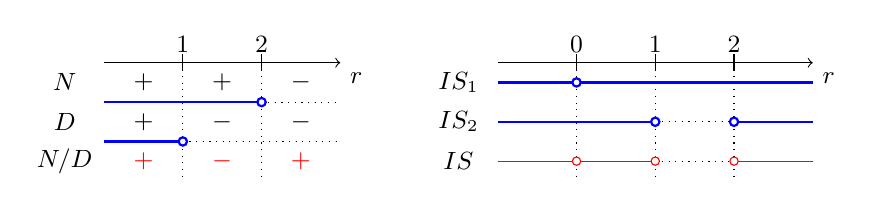
\begin{tikzpicture}[font=\small,x=10mm, y=10mm]

\draw[->] (0,0) -- (3,0) node [below right] () {$r$};
\draw[->] (5,0) -- (9,0) node [below right] () {$r$};

\foreach \x in {1,2,6,7,8}{
\draw(\x,3pt)--(\x,-3pt);
\begin{scope}[dotted]
\draw (\x,0) -- (\x,-1.5);
\draw (2,-.5) -- (3,-.5);
\draw (1,-1) -- (3,-1);
\draw (7,-.75) -- (8,-.75);
\draw (7,-1.25) -- (8,-1.25);
\end{scope}}

\node[above]  at (1,0) {$1$};
\node[above]  at (2,0) {$2$};
\node[above]  at (6,0) {$0$};
\node[above]  at (7,0) {$1$};
\node[above]  at (8,0) {$2$};

\begin{scope}[blue,thick]
\draw (0,-.5) -- (2,-.5);
\draw (1,-1) -- (0,-1);
\draw (5,-.25) -- (6,-.25);
\draw (5,-.25) -- (9,-.25);
\draw (5,-.75) -- (7,-.75);
\draw (8,-.75) -- (9,-.75);

\draw[fill=white] (2,-.5)circle (1.5pt);
\draw[fill=white] (1,-1)circle (1.5pt);
\draw[fill=white] (6,-.25)circle (1.5pt);
\draw[fill=white] (7,-.75)circle (1.5pt);
\draw[fill=white] (8,-.75)circle (1.5pt);
\end{scope}

\foreach \x in {4.5}{
\node  at (\x,-.25) {$IS_1$};
\node  at (\x,-.75) {$IS_2$};
\node  at (\x,-1.25) {$IS$};
}
\foreach \x in {-0.5}{
\node  at (\x,-.25) {$N$};
\node  at (\x,-.75) {$D$};
\node  at (\x,-1.25) {$N/D$};
}

\foreach \z in {.5,1.5}
\node  at (\z,-.25) {$+$};

\foreach \zi in {1.5,2.5}
\node  at (\zi,-.75) {$-$};

\node  at (2.5,-.25) {$-$};
\node  at (0.5,-.75) {$+$};

\begin{scope}[red]
\foreach \y in {-1.25}{
\foreach \ziv in {1.5}
	\node at (\ziv,\y) {$-$};
\foreach \zv in {.5,2.5}
\node at (\zv,\y) {$+$};
\draw (5,-1.25) -- (7,-1.25);
\draw (8,-1.25) -- (9,-1.25);
\draw[fill=white] (6,-1.25)circle (1.5pt);
\draw[fill=white] (7,-1.25)circle (1.5pt);
\draw[fill=white] (8,-1.25)circle (1.5pt);

}
\end{scope}
\end{tikzpicture}

% \end{center}
% ricaviamo$\IS_{2} = \{k \in \insR | k \ldots \ldots \ldots \vee k > 
% \ldots 
% \ldots \ldots \}$
% Dal grafico a destra inoltre otteniamo$\IS = \IS_{1} \cap \IS_{2} = \{ k 
% \in 
% \insR | k
% \ldots \ldots \ldots \vee 0 < k < \ldots \ldots \vee k \ldots \ldots 
% \ldots \}$
% \end{esercizio}
% 
% \begin{esercizio}
%  \label{ese:3.92}
% Assegnata l'equazione~$(k + 1) x^{2} + (k + 3) x + k = 0$ stabilire per 
% quale 
% valore di$k$ una sua soluzione è$x =-1$ In tale caso determinare l'altra 
% soluzione.
% 
% \emph{Traccia di svolgimento}:
% Ricordiamo che un valore numerico è soluzione di un'equazione se 
% sostituito 
% all'incognita trasforma l'equazione in una uguaglianza vera.
% Per questo motivo, sostituendo all'incognita il valore assegnato, il 
% parametro 
%$k$ dovrà verificare l'uguaglianza:$(k + 1) (- 1)^{2} + (k + 3) (- 1) + k = 
% 0 
% \Rightarrow\ldots\ldots\ldots\ldots$
% Sostituendo il valore di$k$ trovato, l'equazione diventa:$3 x^{2} + 5 x + 
% 2 = 
% 0$ l'altra soluzione può essere trovata o con la formula risolutiva, 
% oppure
% ricordando che$x_{1} + x_{2}=- \dfrac{b}{a}=- \dfrac{5}{3}$ da cui 
%$x_{2}=\ldots\ldots$ o anche$x_{1} \cdot x_{2}=\dfrac{c}{a}=\dfrac{2}{3}$ 
% da cui 
%$x_{2}=\ldots\ldots$
% \end{esercizio}
% 
% \begin{esercizio}
%  \label{ese:3.93}
% Giustificare la verità della seguente proposizione: ``per qualunque 
% valore 
% assegnato al parametro$m$ l'equazione~$(m-1) x^{2} + 2 m x + m + 1 = 0$
% ha soluzioni reali distinte''.
% Determinare inoltre$m$ affinché: a)$x_{1} + x_{2} = 1-\sqrt{3}$\quad b)$ 
% x_{1} \cdot x_{2} = \dfrac{12}{5}$\quad c)$x_{1} + x_{2} = 1-x_{1} \cdot 
% x_{2}$
% \end{esercizio}
% 
% \begin{esercizio}
%  \label{ese:3.94}
% Nell'equazione~$7 x^{2} + (k-5) x-(k + 2) = 0$ determinare$k$ affinché le 
% soluzioni siano reali;~ distingui i casi ``reali coincidenti'' e ``reali 
% distinte''.
% Nel primo caso determina$x_{1} = x_{2} = \ldots \ldots$ nel secondo caso, 
% determina$k$ affinché
% \begin{enumeratea}
% \item il prodotto delle soluzioni sia$- \dfrac{8}{3}$
% \item una soluzione sia nulla;~
% \item le soluzioni siano una il reciproco dell'altra, cioè:$x_{1} = \dfrac 
% {1} 
% {x_{2}}$
% \item la somma dei reciproci delle soluzioni sia$\dfrac{1} {2}$
% \item la somma delle soluzioni superi il loro prodotto di$2$
% \end{enumeratea}
% \end{esercizio}
% 
% \begin{esercizio}
%  \label{ese:3.95}
% Verificare che nell'equazione~$(2 m-3) x^{2}-(m + 2) x + 3 m-2 = 0$ si 
% hanno due 
% valori del parametro per cui le soluzioni sono reali coincidenti. 
% Determina i 
% due valori.
% \end{esercizio}
% 
% \begin{esercizio}
%  \label{ese:3.96}
% Nell'equazione~$x^{2}-2 (k + 2) x + (k^{2}-3 k + 2) = 0$ determinare$k$ 
% affinché le soluzioni siano reali, con somma positiva e prodotto negativo.
% 
% \emph{Traccia di svolgimento}:
% Il problema richiede tre condizioni alle quali deve soddisfare 
% contemporaneamente il parametro, pertanto si formalizza con il sistema
%$\left \{ \begin{array}{l} \Delta \geq 0 \\- \dfrac{b}{a} > 0\\
% \dfrac{c}{a} < 0 \end{array}\right.$
% \end{esercizio}

\begin{esercizio}
 \label{ese:3.105}
 Per quale valore di $k \in \insR$ l'equazione~$kx^{2}-x + k = 0$ non 
ammette soluzioni reali?
\[\boxA\;~ k \leq-\dfrac{1}{2} \vee k \geq + \dfrac{1}{2}\quad\boxB\;~ - 
\dfrac{1}{2} 
< k < \dfrac{1}{2}\quad\boxC\;~ k <-\dfrac{1}{2} \vee k > 
\dfrac{1}{2}\quad\boxD\;~ - 
\dfrac{1}{2} \leq k \leq \dfrac{1}{2}\]
\end{esercizio}

\begin{esercizio}
 \label{ese:3.111}
Se l'equazione~$(k + 1) x^{2}-kx-4 = 0$ ha una soluzione uguale a $2$ 
quanto 
vale l'altra soluzione?
\[\boxA\quad x = 0\qquad\boxB\quad x =-2\qquad\boxC\quad x = 
\dfrac{1}{2}\qquad\boxD\quad x = 2\]
\end{esercizio}

\begin{esercizio}[\Ast]
 \label{ese:3.97}
Data l'equazione~$x^{2}-2 x-k = 0$ determinare$k$ in modo che
\begin{enumeratea}
\item le soluzioni siano reali e distinte \quad$(\Delta>0)$
\item la somma delle soluzioni sia $10 \quad (x_{1} + x_{2} = 10)$
\item il prodotto delle soluzioni sia $10 \quad (x_{1} \cdot x_{2} = 10)$
\item una soluzione sia uguale a $0$ \quad (sostituire$0$ alla$x$);~
\item le radici siano opposte \quad $(x_{1} + x_{2} = 0)$
\item le radici siano reciproche \quad $(x_{1} \cdot x_{2} = 1)$
\item le radici siano coincidenti \quad $(\Delta=0)$
\item la somma dei quadrati delle radici sia $12 \quad \left(x_{1}^{2} + 
x_{2}^{2} = (x_{1} + x_{2})^{2}-2x_{1} x_{2} = 12\right)$
\item la somma dei reciproci delle radici sia $-4 \quad 
\left(\dfrac{1}{x_{1}} + 
\dfrac{1}{x_{2}} = \dfrac{x_{1} +x_{2}}{x_{1} x_{2}} =-4 \right)$
\item la somma dei cubi delle radici sia $1$ \protect\\$\left( x_{1}^{3} + 
x_{2}^{3} = (x_{1} + x_{2})^{3}-3x_{1}^{2} x_{2}-3x_{1} x_{2}^{2} = (x_{1} 
+ 
x_{2})^{3}-3x_{1} x_{2} (x_{1} + x_{2}) = 1\right)$
\item le radici siano entrambe negative $\left(\left\{\begin{array}{l} 
x_{1} 
\cdot x_{2} > 0 \\x_{1} + x_{2} < 0 \end{array}\right.\right)$
\end{enumeratea}
\end{esercizio}

\begin{flushright}
$\left[a)~k >-1,\quad b)~\emptyset,\quad c)~k =-10,\quad 
        d)~k = 0,\quad e)~ \emptyset ,\quad f)~ k =-1 ,\quad 
        g)~ k =-1 ,\quad \right.$
       $\left. h)~ k = 4 ,\quad i)~ k = \dfrac{1}{2} ,\quad 
        j)~ k =-\dfrac{7}{6} ,\quad k)~\emptyset\right]$
\end{flushright}

\begin{esercizio}[\Ast]
 \label{ese:3.98}
Data l'equazione~$x^{2}-kx -1 = 0$ determinare $k$ in modo che
\begin{enumeratea}
\item le soluzioni siano coincidenti;~
\item la somma delle radici sia $8$
\item le radici siano opposte;~
\item una radice sia $- \dfrac{1}{3}$
\item il prodotto delle radici sia $-1$
\end{enumeratea}
\end{esercizio}

\begin{flushright}
$\left[a)~\emptyset ,\quad b)~k = 8 ,\quad c)~ k = 0,\quad 
d)~k = \dfrac{8}{3} ,\quad e)~\forall k \in \insR\right]$
\end{flushright}

\begin{esercizio}[\Ast]
 \label{ese:3.99}
Data l'equazione~$x^{2} + (k + 1) x + k = 0$ determinate $k$ affinché 
l'equazione
\begin{enumeratea}
\item abbia una soluzione uguale a zero;~
\item abbia soluzioni opposte;~
\item non abbia soluzioni reali;~
\item abbia le radici reciproche;~
\item abbia le radici positive (regola di Cartesio).
\end{enumeratea}
\end{esercizio}

\begin{flushright}
$\left[a)~ k = 0 ,\quad b)~ k =-1 ,\quad c)~ \emptyset ,\quad 
d)~ k = 1 ,\quad e)~ \emptyset \right]$
\end{flushright}

\begin{esercizio}[\Ast]
 \label{ese:3.100}
Data l'equazione~$x^{2}-kx + 6 = 0$ determinate $k$ affinché
\begin{enumeratea}
\item abbia la somma delle radici uguale a $7$
\item abbia le radici reali e opposte;~
\item abbia la somma dei reciproci delle radici uguale a $-6$
\item abbia una radice uguale a $- \dfrac{3}{2}$
\end{enumeratea}
\end{esercizio}

\begin{flushright}
$\left[a)~ k = 7 ,\quad b)~ \emptyset ,\quad c)~ k =-36 ,\quad 
d)~ k =-\dfrac{11}{2} \right]$
\end{flushright}

% \newpage %-----------------------------------------

\begin{esercizio}[\Ast]
 \label{ese:3.101}
Data l'equazione~$x^{2} + (k + 1) x + k^{2} = 0$ determinare $k$ affinché
\begin{enumeratea}
\item abbia come soluzione $-1$
\item abbia una soluzione doppia $(x_1 =x_2)$
\item abbia le radici reciproche;~
\item abbia una radice l'opposto della reciproca dell'altra 
$\left(x_1=-\dfrac{1}{x_2}\rightarrow x_1 \cdot x_2=-1\right)$
\item abbia una radice nulla.
\end{enumeratea}
\end{esercizio}

\begin{flushright}
$\left[a)~ k = 0 \vee k = 1 ,\quad b)~ k =-\dfrac{1}{3} \vee k = 1 
,\quad c)~ k = \pm 1 ,\quad d)~ \emptyset ,\quad e)~ k=0 \right]$
\end{flushright}

\begin{esercizio}[\Ast]
 \label{ese:3.102}
Data l'equazione~$kx^{2}-2kx + k-2 = 0$ determinare $k$ affinché
\begin{enumeratea}
\item abbia una radice nulla;~
\item abbia la somma dei reciproci delle radici uguale a $1$
\item abbia la somma dei quadrati delle radici uguale a $4$
\item abbia la somma delle radici che superi di $5$ il loro prodotto.
\end{enumeratea}
\end{esercizio}

\begin{flushright}
$\left[a)~ k = 2 ,\quad b)~ k = -2 ,\quad c)~ k = 2 ,\quad 
d)~ k = \dfrac{1}{2} \right]$
\end{flushright}

\begin{esercizio}[\Ast]
 \label{ese:3.103}
Data l'equazione~$x (x-a) = \dfrac{a + x}{a + 2}$ determinate $a$ affinché:
\begin{multicols}{2}
\begin{enumeratea}
\item $x_1 = 1$;
\item l'equazione sia di primo grado;
\item $x_1 = 1 / x_2$;
\item $x_1 + x_2 = 2 \cdot x_1 x_2$;
\item $x_1^2 + x_2^2 = 0$;
\item $x_1 + x_2 = - x_1 x_2$;
\item le soluzioni siano reali e distinte;
\item l'equazione sia spuria;
\item $x_1^3 + x_2^3 = 0$;
\item le soluzioni siano reali e discordi;
\item $1/x_1^3 + 1/x_2^3 = 1$;
\end{enumeratea}
\end{multicols}
\end{esercizio}

\begin{flushright}
$\left[a)~ a =-1 \pm \sqrt{2} ,\quad b)~ \emptyset ,\quad c)~ a 
=-1 ,\quad d)~ a_{1.2} =\dfrac{- 2 \pm \sqrt{3}}{2} ,\quad e)~ \emptyset 
,\quad f)~ \emptyset \right]$
\end{flushright}

\begin{esercizio}[\Ast]
 \label{ese:3.104}
Data l'equazione~$kx^{2}-(2k + 1) x + k-5 = 0$ determinare il valore di~$k$ 
per 
il quale:
\begin{multicols}{2}
\begin{enumeratea}
\item l'equazione abbia soluzioni reali;
\item $x_1 x_2=-2$;
\item $x_1 + x_2 = 1$;
\item $x_1 = -2$;
\item $x_1 = -x_2$;
\item $1/x_1 + 1/x_2 = 3$;
\item $x_1 = 1/x_2$;
\item $x_1 = -1/x_2$;
\item $x_1^2 + x_2^2 = 4$;
\item le radici siano concordi;
\item le radici siano entrambe negative;
\item $x_1 + x_2 = - x_1 x_2$.
\end{enumeratea}
\end{multicols}
\end{esercizio}

\begin{flushright}
$\left[a)~ k \geq-\dfrac{1}{24} ,\quad b)~ k = \dfrac{5}{3} ,\quad 
c)~ k=-1  non accettabile,\quad d)~ k = \dfrac{1}{3} ,\quad e)~ k 
=-\dfrac{1}{2} non accettabile,\quad \right.$
$\left.f)~ k = 16 ,\quad g)~ \emptyset ,\quad 
i)~ k = \dfrac{7 \pm \sqrt{51}}{2} ,\quad j)~ - \dfrac{1}{24} \leq k < 0 
\vee k 
> 5 ,\quad k)~ - \dfrac{1}{24} \leq k < 0 \right]$
\end{flushright}

\begin{esercizio}
 \label{ese:3.106}
Per quale valore di$k \in \insR$ l'equazione~$x^{2} + (k-2) x + 1 = 0$ 
ammette 
due soluzioni reali e distinte?
\[\boxA\quad k > 4\qquad\boxB\quad k = 0 \vee k = 4\qquad\boxC\quad 0 < k < 
4\qquad\boxD\quad k < 0 \vee k > 4\]
\end{esercizio}

\begin{esercizio}
 \label{ese:3.107}
Per quale valore di$k$ l'equazione~$(k-1) x^{2} + kx + (k + 1) = 0$ ha una 
soluzione nulla?
\[\boxA\quad k = 1\qquad\boxB\quad k = -1\qquad\boxC\quad k 
=0\qquad\boxD\quad 
\text{nessun valore di }k\]
\end{esercizio}

\begin{esercizio}
 \label{ese:3.108}
Per quale valore di$k$ l'equazione~$kx^{2} + \dfrac{1}{2} x + 1 = 0$ ha due 
soluzioni identiche?
\[\boxA\quad k = \dfrac{1}{4}\qquad\boxB\quad k = 
\dfrac{1}{16}\qquad\boxC\quad k 
= 2\qquad\boxD\quad \text{nessun valore di }k\]
\end{esercizio}

\begin{esercizio}
 \label{ese:3.109}
Per quale valore di$k$ l'equazione~$(k + 3) x^{2}-2x + k = 0$ ammette due 
soluzioni reciproche?
\[\boxA\quad k = 0\qquad\boxB\quad k = -3\qquad\boxC\quad \text{qualsiasi 
valore 
di }k\qquad\boxD\quad \text{nessun valore di }k\]
\end{esercizio}

\begin{esercizio}
 \label{ese:3.110}
Per quale valore di$k$ l'equazione~$(k + 1) x^{2}-kx-4 = 0$ ha una 
soluzione 
uguale a$2$?
\[\boxA\quad k = 4\qquad\boxB\quad k =-2\qquad\boxC\quad k = 
0\qquad\boxD\quad k 
=-1\]
\end{esercizio}

\begin{multicols}{2}

%===================================

% \subsection*{3.9 - Problemi di secondo grado}
\numnameref{sec:eq2gr_problemi}

\begin{esercizio}[\Ast]
 \label{ese:3.112}
Il quadrato di un numero reale supera la metà del numero stesso di~$5$
Determina i numeri reali che rendono vera la proposizione enunciata.
\hfill$\left[-2;~5/2\right]$
\end{esercizio}

\begin{esercizio}[\Ast]
 \label{ese:3.113}
Il prodotto della metà di un numero relativo con il suo successivo è~$666$
Quali numeri verificano questa proprietà?
\hfill$\left[36;~-37\right]$
\end{esercizio}

\begin{esercizio}
 \label{ese:3.114}
Trova un numero positivo che addizionato al proprio quadrato dia come 
somma~$156$
\hfill$\left[...\right]$
\end{esercizio}

\begin{esercizio}
 \label{ese:3.115}
Un numero addizionato al quadrato della sua metà, dà come risultato~$120$
Trova il numero.
\hfill$\left[...\right]$
\end{esercizio}

\begin{esercizio}
 \label{ese:3.116}
Verifica che non esiste alcun numero reale tale che il quadrato del suo
doppio uguagli la differenza tra il triplo del suo quadrato e il quadrato
della somma del numero con~$3$
\hfill$\left[...\right]$
\end{esercizio}

\begin{esercizio}[\Ast]
 \label{ese:3.117}
Due numeri naturali hanno rapporto~$2/3$ e somma dei loro quadrati~$3757$
Individua i numeri che verificano questa proprietà.
\hfill$\left[51;~34\right]$
\end{esercizio}

\begin{esercizio}[\Ast]
 \label{ese:3.118}
La somma dei quadrati di due numeri pari consecutivi è~$580$ Quali sono i
due numeri?
\hfill$\left[16;~18\right]$
\end{esercizio}

\begin{esercizio}[\Ast]
 \label{ese:3.119}
Di due numeri naturali consecutivi si sa che la somma dei loro reciproci
è~$9/20$ Quali sono i due numeri?
\hfill$\left[4;~5\right]$
\end{esercizio}

\begin{esercizio}[\Ast]
 \label{ese:3.120}
Di cinque numeri interi consecutivi si sa che la differenza tra il quadrato
della somma degli ultimi due numeri e la somma dei quadrati dei primi tre è
$ 702$ Qual è il più piccolo di questi numeri?
\hfill$\left[17\right]$
\end{esercizio}

 \begin{esercizio}[\Ast]
 \label{ese:3.121}
La somma delle età di un padre con quella del figlio è~$34$ Sapendo che
l'età del padre aumentata di~$8$ anni dà il quadrato dell'età del figlio,
trovare le due età.
\hfill$\left[28;~6\right]$
\end{esercizio}

\begin{esercizio}[\Ast]
 \label{ese:3.122}
Determina due numeri naturali sapendo che la somma tra il doppio del minore
ed il triplo del maggiore è~$42$ e che il rapporto tra la loro somma e il 
loro
prodotto è~$5/12$
\hfill$\left[3;~12\right]$
\end{esercizio}

\begin{esercizio}[\Ast]
 \label{ese:3.123}
Trova l'età di una persona sapendo che fra tre anni la sua età sarà
uguale al quadrato della quinta parte dell'età che aveva tre anni fa.
\hfill$\left[33\right]$
\end{esercizio}

\begin{esercizio}[\Ast]
 \label{ese:3.124}
Trova due numeri pari consecutivi tali che la somma del quadrato del minore
con il loro prodotto sia~$544$
\hfill$\left[16;~18\right]$
\end{esercizio}

\begin{esercizio}[\Ast]
 \label{ese:3.125}
Trova due numeri naturali sapendo che il minore supera di~$2$ la terza parte
del maggiore e che il quadrato del maggiore supera di~$68$ il quadrato del
doppio del minore.
\hfill$\left[8;~18\right]$
\end{esercizio}

\begin{esercizio}[\Ast]
 \label{ese:3.126}
Da un segmento di~$25\unit{cm}$ ne vogliamo ottenere due in modo che la 
somma 
dei loro quadrati sia~$337$
\hfill$\left[9;~16\right]$
\end{esercizio}

\begin{esercizio}[\Ast]
 \label{ese:3.127}
In una frazione il numeratore e il denominatore hanno somma~$14$, mentre la
somma dei loro quadrati è~$106$ Qual è la frazione?
\hfill$\left[5/9;~9/5\right]$
\end{esercizio}
% 
% \begin{esercizio}[\Ast]
%  \label{ese:3.128}
% Due navi partono contemporaneamente da uno stesso porto e arrivano alla
% stessa destinazione dopo aver percorso sulla stessa rotta a velocità
% costante~$720\unit{miglia}$ Sapendo che una delle due navi viaggia con 
% una 
% velocità
% di 1 nodo (1 miglio all'ora) superiore a quella dell'altra nave e che 
% perciò
% arriva 3 ore prima a destinazione, determina le velocità in nodi delle due
% navi.
% \hfill$\left[15;~16\right]$
% \end{esercizio}
% 
% \begin{esercizio}
%  \label{ese:3.129}
% Due navi che viaggiano su rotte perpendicolari a velocità costante si
% incontrano in mare aperto. Sapendo che una delle navi viaggia a 15 nodi (1
% nodo = 1 miglio all'ora), dopo quanto tempo le due navi si trovano alla
% distanza di 40 miglia?
% \hfill$\left[...\right]$
% \end{esercizio}
% 
% \begin{esercizio}
%  \label{ese:3.130}
% Luca e Carlo bevono due aranciate in bottiglia. Nel tempo in cui Luca beve
% 11 sorsi, Carlo ne beve 8, ma due sorsi di Carlo equivalgono a tre di 
% Luca.
% Quando Carlo inizia a bere Luca ha già preso 4 sorsi. Dopo quanti sorsi di
% Carlo le due bibite hanno lo stesso livello?
% \hfill$\left[...\right]$
% \end{esercizio}
% 
% \begin{esercizio}
%  \label{ese:3.131}
% Un maratoneta durante un allenamento fa due giri di un percorso 
% di~$22\unit{km} 
% $
% mantenendo in ciascun giro una velocità costante ma nel secondo giro la
% velocità è inferiore di~$0,5\unit{km/h}$ rispetto al primo giro. A quali 
% velocità
% ha corso se ha impiegato complessivamente 2 ore e un quarto?
% \hfill$\left[...\right]$
% \end{esercizio}
% 
% \begin{esercizio}[\Ast]
%  \label{ese:3.132}
% Un capitale di 12000 euro è depositato in banca a un certo tasso di 
% interesse
% annuale. Alla scadenza del primo anno gli interessi maturati vengono
% ridepositati sullo stesso conto. Alla scadenza del secondo anno si ritira 
% la
% somma di 12854,70 euro. Qual è stato il tasso di interesse?
% \hfill$\left[3,5\%\right]$
% \end{esercizio}
% 
% \begin{esercizio}
%  \label{ese:3.133}
% In un rettangolo, se si aumenta di 2 metri la base e si riduce di un metro
% l'altezza, la sua area aumenta di 4 metri quadrati. Se invece si riduce di
% un metro la base e si aumenta di 2 metri l'altezza, l'area aumenta di 22
% metri quadrati. Quali sono le dimensioni del rettangolo?
% \hfill$\left[...\right]$
% \end{esercizio}
% 
% \begin{esercizio}[\Ast]
%  \label{ese:3.134}
% Una ditta spende mensilmente 73500 in stipendi per i propri dipendenti.
% Aumentando di 5 il numero dei dipendenti, ma riducendo l'orario di lavoro,
% diminuisce a ciascuno lo stipendio di 200 e spende solamente 2500 in più 
% per
% gli stipendi. Quanti dipendenti aveva inizialmente la ditta e quanto
% guadagnava ognuno di essi?
% \hfill$\left[35;~2100\right]$
% \end{esercizio}

\begin{esercizio}[\Ast]
 \label{ese:3.135}
Da un cartoncino rettangolare (~$ABCD$, come in figura) si vuole ritagliare 
un
quadrato (~$DEFG$) in modo che le due parti ottenute siano equivalenti.
Determinare la misura del lato del quadrato sapendo che
$\overline {EC} = 6\unit{cm}$ e$\overline {AG} = 4\unit{cm}$
\begin{center}
 % (c) 2013 Claudio Carboncini - claudio.carboncini@gmail.com
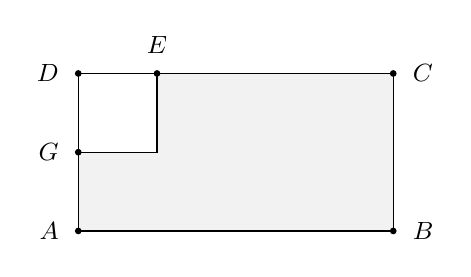
\begin{tikzpicture}[x=10mm,y=10mm,font=\small]

  \fill[fill=gray!10] (1,1) rectangle (5,3);
  \fill[fill=white] (1,3) rectangle (2,2);
  \draw (1,1) rectangle (5,3);
  \draw (1,3) rectangle (2,2);
  \node [label={[name=label node]left:$A$}] at (1,1) {};
  \node [label={[name=label node]left:$D$}] at (1,3) {};
  \node [label={[name=label node]right:$C$}] at (5,3) {};
  \node [label={[name=label node]right:$B$}] at (5,1) {};
  \node [label={[name=label node]left:$G$}] at (1,2) {};
  \node [label={[name=label node]above:$E$}] at (2,3) {};

  \foreach \x in {1,5}
    \foreach \y in {1,3}
      \filldraw[fill=black, draw=black]  (\x,\y) circle (1pt);
      \filldraw[fill=black, draw=black]  (1,2) circle (1pt);
      \filldraw[fill=black, draw=black]  (2,3) circle (1pt);

\end{tikzpicture}

\end{center}
\hfill$\left[...\right]$
\end{esercizio}

\begin{esercizio}[\Ast]
 \label{ese:3.136}
Un terreno a forma rettangolare di$6016\unit{m^2}$ viene recintato con un 
muro 
lungo~$350\unit{m}$ Quali sono le dimensioni del rettangolo?
\hfill$\left[47;~128\right]$
\end{esercizio}

\begin{esercizio}[\Ast]
 \label{ese:3.137}
Determinare sul segmento~$AB$ di misura~$5\unit{m}$ un punto~$P$ tale che 
il rettangolo delle due parti sia equivalente al quadrato di 
lato~$2\unit{m}$ Rappresenta con un disegno le soluzioni.
\hfill$\left[1\unit{cm};~4\unit{cm}\right]$
\end{esercizio}

\begin{esercizio}[\Ast]
 \label{ese:3.138}
Calcolare perimetro e area del triangolo~$ABC$ isoscele sulla base~$AB$ 
sapendo
che la differenza tra la base e l'altezza ad essa relativa è~$0,5\unit{m}$ 
e 
tale
è anche la differenza tra il lato~$CB$ e la base stessa.
\hfill$\left[2p=25\unit{m};~A=30\unit{m^2}\right]$
\end{esercizio}

\begin{esercizio}[\Ast]
 \label{ese:3.139}
La superficie del rettangolo~$ABCD$ supera di~$119\unit{m^2}$ la superficie 
del quadrato
costruito sul lato minore~$AD~$Determinare il perimetro e la misura della
diagonale sapendo che i~$7/10$ del lato maggiore AB sono uguali ai~$12/5$ 
del
lato minore.
\hfill$\left[2p=62\unit{m};~d=25\unit{m}\right]$
\end{esercizio}

\begin{esercizio}[\Ast]
 \label{ese:3.140}
Nel trapezio rettangolo~$ABCD$, il rapporto tra la base maggiore~$AB$ e la 
base
minore~$CD$ è~$8/5$, il lato obliquo forma con~$AB$ un angolo di$ 
45\grado~$Determinare il perimetro sapendo che l'area è$312\unit{m^2}$
\hfill$\left[2p = 64 + 12 \sqrt{2}\right]$
\end{esercizio}

\begin{esercizio}[\Ast]
 \label{ese:3.141}
Determina il perimetro di un rombo che ha l'area di$24\unit{m^2}$ e il 
rapporto 
tra le diagonali~$4/3$
\hfill$\left[40\unit{m}\right]$
\end{esercizio}

\begin{esercizio}[\Ast]
 \label{ese:3.142}
Un rettangolo~$ABCD$ ha il perimetro di~$48\unit{cm}$ e l'area di$ 
128\unit{cm^2}~$A una certa
distanza$x$ dal vertice~$A$ sui due lati~$AD$ e~$AB$ si prendono 
rispettivamente i
punti~$P$ e$ Q~$Alla stessa distanza$ x$ dal vertice~$C$ sui lati~$CB$ 
e~$CD$ si
prendono rispettivamente i punti$ R$ e$ S$ Sapendo che il rapporto tra 
l'area
del rettangolo~$ABCD$ e l'area del quadrilatero~$PQRS$ è~$32/23$ calcola 
la
distanza$x$
\hfill$\left[6\unit{cm}\right]$
\end{esercizio}

\begin{esercizio}
 \label{ese:3.143}
Un trapezio rettangolo ha la base minore di~$9|unit{cm}$, l'altezza i~$2/9$ 
della base
maggiore e l'area di$20 + 9 \sqrt{2}\unit{cm^{2}}~$Determina la misura 
della 
base maggiore.
\hfill$\left[...\right]$
\end{esercizio}

\begin{esercizio}[\Ast]
 \label{ese:3.144}
Da un quadrato di~$32\unit{cm}$ di lato vengono ritagliati due triangoli 
rettangoli
come descritti in figura. Calcola la misura di $x$,
inferiore alla metà del lato del quadrato, in modo che l'area totale dei
due triangoli evidenziati sia pari a~$344\unit{cm^2}$
\begin{center}
 % (c) 2013 Claudio Carboncini - claudio.carboncini@gmail.com
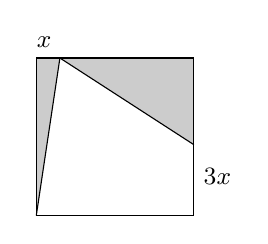
\begin{tikzpicture}[x=10mm,y=10mm,font=\small]

  \fill[fill=gray!40] (1,1) -- (1,3) -- (1.3,3);
  \fill[fill=gray!40] (1.3,3) -- (3,3) -- (3,1.9);
  \draw (1,1) rectangle (3,3);
  \draw (1.3,3)--(1,1);
  \draw (3,1.9)--(1.3,3);
  \node (x) at (1.1,3.2) {$x$};
  \node (h) at (3.3,1.5) {$3x$};

\end{tikzpicture}

\end{center}
\vspace*{-2em}
\hfill$\left[...\right]$
\end{esercizio}

\begin{esercizio}[\Ast]
 \label{ese:3.145}
Il rettangolo~$ABCD$ ha l'area di~$558\unit{cm^2}$ e il lato~$DC$ di$ 
18\unit{cm}$ Lo si
vuole trasformare in un nuovo rettangolo~$AEFG$ accorciando l'altezza di 
una 
quantità~$5x$ e allungando la base di una quantità~$4x$ in modo che il 
nuovo 
rettangolo~$AEFG$ che abbia l'area di~$228\unit{cm^2}~$.
Determina la quantità$ x$ necessaria a compiere la trasformazione richiesta.
\hfill$\left[5\unit{cm}\right]$
\end{esercizio}
% 
% \begin{esercizio}[\Ast]
%  \label{ese:3.146}
% Il rettangolo~$AEFG$ ha l'area di~$768\{cm^2\}$ e l'altezza~$AG$ di$ 
% 24\unit{cm}$. Si vuole allungare l'altezza di una quantità
% $ x$ e accorciare la base di una quantità doppia~$2x$ in modo da ottenere 
% un
% secondo rettangolo~$ABCD$ che abbia l'area 
% di~$702\unit{cm^2}~$Determina~$x$.
% \hfill$\left[3\unit{cm}\right]$
% \end{esercizio}

\begin{esercizio}
 \label{ese:3.147}
Un trapezio isoscele di area~$144\unit{cm^2}$ ha la base maggiore che 
supera 
di~$10\unit{cm}$
la base minore che a sua volta supera di~$10\unit{cm}$ l'altezza. Determina 
il 
perimetro del trapezio.
\hfill$\left[...\right]$
\end{esercizio}
% 
% \begin{esercizio}[\Ast]
%  \label{ese:3.148}
% Il rettangolo~$ABCD$ ha l'area di~$240\unit{cm^2}$ e l'altezza~$AD$ di$ 
% 12\unit{cm}$ Si
% vuole trasformare il rettangolo in un triangolo~$AEF$ allungando l'altezza 
% di 
% una quantità~$3x$ e accorciando la
% base di una quantità$ x$ (vedi figura) in modo che il nuovo 
% triangolo~$AEF$ 
% abbia l'area di~$162\unit{cm^2}$
% \begin{center}
%  % (c) 2013 Claudio Carboncini - claudio.carboncini@gmail.com
\begin{tikzpicture}[x=10mm,y=10mm,font=\small]
  \draw (1,1) rectangle (5,2);
  \draw (1,1)--(2.6,4.4);
  \draw (4.2,1)--(2.6,4.4);
  \draw (2.6,2)--(2.6,4.4);
  \draw [dotted] (2.6,2) -- (2.6,1);
  \node (x) at (4.7,.7) {$x$};
  \node (h) at (2.3,3) {$3x$};
  \node [label={[name=label node]below left:$A$}] at (1,1) {};
  \node [label={[name=label node]above left:$D$}] at (1,2) {};
  \node [label={[name=label node]above right:$C$}] at (5,2) {};
  \node [label={[name=label node]below right:$B$}] at (5,1) {};
  \node [label={[name=label node]below:$E$}] at (4.2,1) {};
  \node [label={[name=label node]above:$F$}] at (2.6,4.4) {};

  \foreach \x in {1,5}
    \foreach \y in {1,2}
      \filldraw[fill=black, draw=black]  (\x,\y) circle (1pt);
      \filldraw[fill=black, draw=black]  (2.6,4.4) circle (1pt);
      \filldraw[fill=black, draw=black]  (4.2,1) circle (1pt);

\end{tikzpicture}

% \end{center}
% \hfill$\left[2;~14\text{ non accettabile}\right]$
% \end{esercizio}

\begin{esercizio}[\Ast]
 \label{ese:3.149}
La piramide di Cheope è a base quadrata ed ha una superficie totale pari a
$ 135700\unit{m^2}$ Sapendo che l'apotema della piramide misura~$180$ 
metri, 
si
calcoli la lunghezza del lato di base.
\hfill$\left[230\unit{m}\right]$
\end{esercizio}

\begin{esercizio}[\Ast]
 \label{ese:3.150}
Un container a forma di parallelepipedo a base quadrata ha una superficie
totale pari a~$210\unit{m^2}$ L'altezza è il doppio del lato di base 
diminuito 
di $2$ metri. Trovare la lunghezza del lato di base.
\hfill$\left[5\unit{m}\right]$
\end{esercizio}

% \subsection*{3.10 - Problemi con un parametro}
% 
% \begin{esercizio}
%  \label{ese:3.151}
% Sul prolungamento dei lati~$AB$,~$BC$,~$CD$,~$DA$ del quadrato~$ABCD$ 
% prendi rispettivamente i punti$ Q$,$ R$,$ S$,~$P$ in modo che$ 
% QB=RC=SD=PA~$Dimostra che~$PQRS$ è un quadrato;~ nell'ipotesi che sia$AB 
% = 
% 3\unit{m}$ determina$\overline {AP}$ in modo che l'area di~$PQRS$ sia$ 
% k$, 
% con$ k$ reale positivo.
% \begin{center}
%  % (c) 2013 Claudio Carboncini - claudio.carboncini@gmail.com
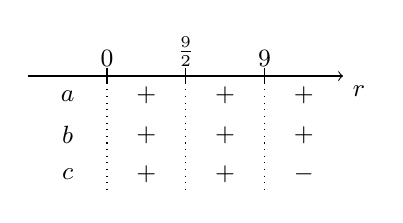
\begin{tikzpicture}[font=\small,x=10mm, y=10mm]

\draw[->] (0,0) -- (4,0) node [below right] () {$r$};

\foreach \x in {1,2,3}{
\draw(\x,3pt)--(\x,-3pt);
\begin{scope}[dotted]
\draw (\x,0) -- (\x,-1.5);
\end{scope}}

\node[above]  at (1,0) {$0$};
\node[above]  at (2,0) {$\frac 9 2$};
\node[above]  at (3,0) {$9$};

\foreach \x in {0.5}{
\node  at (\x,-.25) {$a$};
\node  at (\x,-.75) {$b$};
\node  at (\x,-1.25) {$c$};
}

\foreach \z in {1.5,2.5,3.5}
\node  at (\z,-.25) {$+$};

\foreach \zi in {1.5,2.5,3.5}
\node  at (\zi,-.75) {$+$};

\node  at (1.5,-1.25) {$+$};
\node  at (2.5,-1.25) {$+$};
\node  at (3.5,-1.25) {$-$};
\end{tikzpicture}

% \end{center}
% \emph{Svolgimento}:
% per dimostrare che~$PQRS$ è un quadrato dobbiamo dimostrare che i lati 
% sono
% congruenti e che gli angoli sono retti. Se si pone$\overline{AP} = x$ 
% con$x > 
% 0$
%$\Area(PQRS)= \overline {PQ}^{2} = \overline {PA}^{2} + 
% \overline{AQ}^{2}$per il 
% teorema di Pitagora.
% Verifica che si ottiene l'equazione risolvente$2 x^{2} + 6 x + (9-k) = 0$ 
% Poiché vogliamo soluzioni reali positive, discuti l'equazione con il 
% metodo di 
% Cartesio. Il discriminante è$\Delta = 36-8 (9-k)$ pertanto l'equazione 
% ammette 
% soluzioni reali per$k \geq \dfrac{9}{2}~$Dal segno dei coefficienti, 
% essendo i 
% primi due coefficienti positivi si ha una permanenza e quindi una radice 
% negativa che non è accettabile. Per ottenere una soluzione positiva ci 
% deve 
% essere una variazione di segno negli ultimi due coefficienti, in altre 
% parole 
%$9-k$ deve essere negativo cioè$9-k < 0 \rightarrow k > 9~$Pertanto il 
% problema 
% ha soluzioni per$k > 9$
% \end{esercizio}
% 
% \begin{esercizio}
%  \label{ese:3.152}
% Nel trapezio rettangolo~$ABCD$ di base maggiore~$BC$, la diagonale~$AC$ è 
% bisettrice dell'angolo$B \widehat {C} D~$Posto$\overline {AB} = 
% 1\unit{m}$, 
% determina la base maggiore in modo che sia~$2k$ il perimetro del 
% trapezio. 
% Imposta dati e obiettivo del problema.
% \begin{center}
%  % (c) 2013 Claudio Carboncini - claudio.carboncini@gmail.com
\begin{tikzpicture}[x=10mm,y=10mm,font=\small]

  \coordinate(a) at (0,2.598);%il punto A
  \coordinate(b) at (0,0);%il punto B
  \coordinate(c) at (4.5,0);%il punto C
  \coordinate(d) at (3,2.598);%il punto D
  \coordinate (h) at ($(a)!(d)!(c)$);%trova le coordinate della proiezione di D su a--c
  \coordinate (h1) at ($(a)!{1/2}!(h)$);
  \coordinate (h2) at ($(h)!{1/2}!(c)$);
  \coordinate (a1) at ($(a)!{1/2}!(d)$);
  \coordinate (d1) at ($(d)!{1/2}!(c)$);
  \draw (a) -- (b)  -- (c) -- (d) -- cycle;%disegna il trapezio
  \draw [] (d) -- (h);%perpendicolare da D a a--c
  \draw [] (a) -- (c);%la diagonale del trapezio
  \draw (h1) node {$//$} ;
  \draw (h2) node {$//$} ;
  \draw (a1) node {$\times$} ;
  \draw (d1) node {$\times$} ;
  \draw (4.1,0.4) node {$\bullet$} ;
  \draw (3.95,0.12) node {$\bullet$} ;
  \node [label={[name=label node]above:$A$}] at (a) {};
  \node [label={[name=label node]below:$B$}] at (b) {};
  \node [label={[name=label node]below:$C$}] at (c) {};
  \node [label={[name=label node]above:$D$}] at (d) {};
  \node [label={[name=label node]below:$H$}] at (h) {};

\end{tikzpicture}

% \end{center}
% \emph{Svolgimento}: poniamo$\overline {BC} = x~$Dall'informazione che la 
% diagonale~$AC$ è bisettrice dell'angolo$B \widehat {C} D$, possiamo 
% dimostrare che~$ADC$ è un triangolo isoscele sulla base~$AC$ L'equazione 
% risolvente sarà determinata dalla relazione tra i lati che esprime il 
% perimetro 
% del trapezio. Dobbiamo quindi esprimere$\overline {DC}$ in funzione di$ 
% x$ 
% Traccia l'altezza~$DH$ del triangolo isoscele~$ADC$ e dopo aver 
% dimostrato 
% la similitudine di~$ABC$ con~$DHC$, osserva che si ha$DC : AC = HC : BC$ 
% poiché$HC = \dfrac{1}{2} AC$ si ha$\dfrac{1}{2} \overline {AC}^{2} = 
% \overline 
% {DC} \cdot \overline {BC}$ da cui si può ricavare la misura di~$DC = 
% \dfrac{1}{2} \dfrac{AC^{2}}{BC}~$Dato che$\overline {AC}^{2}=1+x^2$, per 
% il 
% teorema di Pitagora applicato al triangolo~$ABC$, quindi~$DC = \dfrac{1 + 
% x^2} 
% {2 x}$ L'equazione parametrica risolvente è$2 x^{2} + x \cdot (1-2 k) + 1 
% = 0$ 
% con$x > 0$ che può essere discussa con il metodo di Cartesio.
% \end{esercizio}
% 
% \begin{esercizio}
%  \label{ese:3.153}
% Il quadrilatero~$ABCD$ ha le diagonali perpendicolari ed è inscritto in 
% una 
% circonferenza;~ sapendo che$\overline{AB} = 5a$$\overline {AE} = 3 a$$2 
% p_{BCA} = \dfrac{5}{2} \cdot \overline {BD}$, essendo$ E$ punto 
% d'incontro 
% delle diagonali, determinate la misura delle diagonali. Poni$\overline 
% {CE} = 
% x$
% \end{esercizio}
% 
% \begin{esercizio}
%  \label{ese:3.154}
% Il rettangolo~$ABCD$ ha i lati~$AB$ e~$BC$ che misurano rispettivamente$ 
% a$ e~$3a$ (con~$a\geq 0$). Prolunga il lato~$AB$ di due segmenti 
% congruenti~$BN$ e~$AM$ e sia$ V$ il punto di intersezione delle retta$ MD 
%$ e~$CN~$Posto$\overline {BN} = x$, determina la misura della base$ MN$ 
% del 
% triangolo$ MVN$ in modo che la sua area sia$ k$ volte l'area del 
% rettangolo 
% assegnato.
% \end{esercizio}
% 
% \begin{esercizio}
%  \label{ese:3.155}
% Due numeri reali hanno come somma~$a$ con$(a \in \insR_{0})$ determinare 
% i 
% due numeri in modo che il loro prodotto sia$ k$ con$(k \in \insR_{0})$ 
% Quale 
% condizione si deve porre sull'incognita? Per quale valore del parametro i 
% due 
% numeri soluzione sono uguali?
% \end{esercizio}
% 
% \begin{esercizio}
%  \label{ese:3.156}
% In un triangolo rettangolo l'altezza~$AH$ relativa all'ipotenusa~$BC$ 
% misura 
%~$1\unit{m}$ e$A \widehat {B} C = 60\grado~$Determinare sulla 
% semiretta~$AH 
%$, esternamente al triangolo, un punto~$P$ in modo che sia$ k$ la somma 
% dei 
% quadrati delle distanze di~$P$ dai vertici del triangolo. Quale condizione 
% va 
% imposta al parametro$ k$ perché il problema abbia significato?
% \end{esercizio}
% 
% \begin{esercizio}
%  \label{ese:3.157}
%$\overline {AB} = 16 a$$\overline {BC} = 2 a \sqrt{14}$ rappresentano le 
% misure 
% dei lati del rettangolo~$ABCD$ determinare un punto~$P$ del segmento~$AB$ 
% tale che la somma dei quadrati delle sue distanze dai vertici~$C$ e~$D$ 
% sia 
% uguale al quadrato della diagonale~$DB$ Posto$\overline {AP} = x$ quale 
% delle 
% seguenti condizioni deve rispettare la soluzione? Dopo aver risolto il 
% problema 
% spiegare il significato delle soluzioni ottenute.
% \end{esercizio}
% 
% \begin{esercizio}
%  \label{ese:3.158}
% Ad una sfera di raggio~$1\unit{m}$ è circoscritto un cono il cui volume è$ 
% k 
%$ volte il volume della sfera. Determina l'altezza del cono.
% \begin{center}
%  % (c) 2013 Claudio Carboncini - claudio.carboncini@gmail.com
\begin{tikzpicture}[x=10mm,y=10mm,font=\small,scale=1.3]

  \coordinate(a) at (0,0);%il punto A
  \coordinate(v1) at (70:5);%il punto V1
  \coordinate(o) at (35:1.5);%il centro del cerchio O
  \coordinate(h) at (1.23,0);%il punto H
  \coordinate (b) at (2.46,0);%il punto B
  \coordinate(v2) at (1.23,6);%il punto v2
  \coordinate (v) at (intersection of a--v1 and h--v2);
  \coordinate (c) at ($(v)!(o)!(b)$);%trova le coordinate della proiezione di o su v--b
  \draw[] (o) circle (0.86);%disegna il cerchio di centro
  \draw[] (v) -- (a) -- (b) -- cycle;%disegna v2--h--a
  \draw[dashed] (v) -- (h);%disegna v--h
  \draw[dashed] (o) -- (c);%disegna o--c
  \draw (h) ellipse (1.23cm and 0.4cm);
  \node [label={[name=label node]above:$V$}] at (v) {};
  \node [label={[name=label node]left:$A$}] at (a) {};
  \node [label={[name=label node]below:$H$}] at (h) {};
  \node [label={[name=label node]right:$B$}] at (b) {};
  \node [label={[name=label node]left:$O$}] at (o) {};
  \node [label={[name=label node]right:$C$}] at (c) {};
\begin{comment}
  \coordinate (h2) at ($(h)!{1/2}!(c)$);
  \coordinate (a1) at ($(a)!{1/2}!(d)$);
  \coordinate (d1) at ($(d)!{1/2}!(c)$);
  \draw (a) -- (b)  -- (c) -- (d) -- cycle;%disegna il trapezio
  \draw [] (d) -- (h);%perpendicolare da D a a--c
  \draw [] (a) -- (c);%la diagonale del trapezio
  \draw (h1) node {$//$} ;
  \draw (h2) node {$//$} ;
  \draw (a1) node {$\times$} ;
  \draw (d1) node {$\times$} ;
  \draw (4.1,0.4) node {$\bullet$} ;
  \draw (3.95,0.12) node {$\bullet$} ;
\end{comment}
\end{tikzpicture}

% \end{center}
% 
% \emph{Dati}:$ \overline {OC} = 1$,$ \overline {OC} = \overline {OH}$,$ OC 
% \perp VB$,\protect\\$ \overline {BC} = \overline {BH}$,$ \overline {AH} = 
% \overline {HB}$,$ VH \perp AB$,\protect\\$ \text{Volume(cono)} = k \cdot 
% \text{Volume(sfera)}$
% 
% \emph{Obiettivo}:$\overline {VH}$
% 
% \emph{Svolgimento}: Poniamo$\overline {VO} = x$ con$x > 0$ da 
% cui$\overline 
% {VH}= \overline {VO} + \overline {OH} = x + 1$
% 
% Ricordiamo che$V\text{(cono)} = \dfrac{1}{3} \pi \overline {HB}^{2} \cdot 
% \overline {VH}$ e$V\text{(sfera)} = \dfrac{4}{3} \pi \overline 
% {CO}^{3}~$Per 
% impostare l'equazione risolvente dobbiamo cercare di esprimere$\overline 
% {HB}^{2}$ in funzione di$ x$ Verifica che dalla similitudine di$ VOC$ 
% con$ 
% VHB$ si deduce:$\overline {HB} : \overline {OC} = \overline {VH} : 
% \overline{VC}$ quindi$\overline {HB} = \dfrac{\overline {OC} \cdot 
% \overline
% {VH}}{\overline {VC}}$ dobbiamo ancora ricavare$\overline {VC}$ che per 
% il 
% teorema di Pitagora su$ VCO$ è \ldots Sostituendo tutti gli elementi 
% trovati 
% nella relazione che lega il volume del cono con il volume della sfera, 
% verifica 
% che si ottiene$x^{2} + 2 x (1-2 k) + 4 k = 0$ con$x > 0$, da discutere con 
% il 
% metodo di Cartesio.
% \end{esercizio}
% 
\end{multicols}
% \begin{esercizio}[\Ast]
%  \label{ese:3.159}
%  Scheda di ripasso sulle equazioni
% \begin{enumerate}
% 	\item L'equazione~$25x^{2} + 1 = 0$ ha per soluzioni:
% 
% \boxA\quad$ x = \pm 5$\qquad \boxB\quad$x = \pm 
% \dfrac{1}{5}$\qquad\boxC\quad 
%$x = 4 \vee x = 1$\qquad\boxD\quad non ha soluzioni reali
% 
% 	\item L'equazione~$16x^{2} + x = 0$ ha per soluzioni:
% 
% \boxA\quad$ x = 4 \vee x = 1$\quad \boxB\quad$x = \pm 
% \dfrac{1}{4}$\quad\boxC\quad$x =-\dfrac{1}{16} \vee x = 0$\quad\boxD\quad 
% non ha 
% soluzioni reali
% 
% 	\item L'equazione~$4x^{2}-9x = 0$ ha per soluzioni:
% 
% \boxA\quad$ x = \pm \dfrac{3}{2}$\qquad \boxB\quad$x = \pm 
% \dfrac{9}{4}$\qquad\boxC\quad$x = \dfrac{3}{2} \vee x = 
% 0$\qquad\boxD\quad$x = 
% \dfrac{9}{4} \vee x = 0$
% 
% 	\item L'equazione~$9x^{2} + 6x + 1 = 0$ ha per soluzioni:
% 
% \boxA\quad$x = \pm 3$\qquad\boxB\quad$x = \pm 
% \dfrac{1}{3}$\qquad\boxC\quad$x 
% =-\dfrac{1}{3}$ doppia\qquad\boxD\quad non ha soluzioni reali
% 
% 	\item L'equazione~$x^{2}-6x + 36 = 0$ ha per soluzioni:
% 
% \boxA\quad$x = \pm 6$\qquad\boxB\quad$x = \pm \sqrt{6}$\qquad\boxC\quad$x 
% =6$ 
% doppia\qquad\boxD\quad non ha soluzioni reali
% 
% 	\item Quale di queste equazioni ammette una soluzione doppia$ x=3$?
% 
% \boxA\quad$2x^{2}-12x + 18 = 0$\quad\boxB\quad$9-x^{2} = 
% 0$\quad\boxC\quad 
%$x^{2} + 6x + 9 = 0$\quad\boxD\quad~$3x^{2} + 9x = 0$
% 
% 	\item Quale equazione di secondo grado si ottiene con soluzioni$ 
% x_1=1 
%$ e$ x_2=3$?
% 
% \boxA\quad$x^{2} + x-1 = 0$\quad\boxB\quad$x^{2}-4x + 3 = 
% 0$\quad\boxC\quad 
%$x^{2}-4x-3 = 0$\quad\boxD\quad$ x^{2} + 4x-3 = 0$
% 
% 	\item Il polinomio$x^{2} + 5x + 6$ può essere scomposto in:
% 
% \boxA\;~$(x + 2) (x-3)$\quad\boxB\;~$(x + 5) (x + 1)$\quad\boxC\;~$(x-2) 
% (x-3)$\quad\boxD\;~ nessuna delle risposte precedenti
% 
% 	\item Una delle soluzioni dell'equazione~$x^{2}-(\sqrt{2} + 1) x + 
% \sqrt{2} = 0$ è$\sqrt{2}$, quanto vale l'altra?
% 
% \boxA\quad$ - \sqrt{2}$\qquad 
% \boxB\quad$\dfrac{1}{\sqrt{2}}$\qquad\boxC\quad 
%$\sqrt{2} + 1$\qquad\boxD\quad$1$
% 
% 	\item Per quale valore di$ k$ l'equazione~$(2k-1) x^{2} + (2k + 1) x 
% + 
% k-2 = 0$ diventa di I° grado?
% 
% \boxA\quad$k = \dfrac{1}{2}$\qquad \boxB\quad$k 
% =-\dfrac{1}{2}$\qquad\boxC\quad 
%$k = 2$\qquad\boxD\quad$k = 0$
% 
% 	\item L'equazione~$4m^{2} x^{2}-5mx + 1 = 0$ con parametro$ m$ ha 
% per 
% soluzioni:
% 
% \boxA\;~$x = m \vee x = 4m$\quad \boxB\;~$x = \dfrac{1}{m} \vee x = 
% \dfrac{1}{4m}$\quad\boxC\;~$x = 64m \vee x = 1$\quad\boxD\;~$x = m \vee x 
% = 
% \dfrac{1}{4}$
% 
% 	\item L'equazione di secondo grado$x^{2} + (a + 1) x + a = 0$ 
% con~$a$ 
% parametro reale ha come soluzioni:
% 
% \boxA\;~$x = 1 \vee x = a$\quad \boxB\;~$x = a-1 \vee x = 
% 1$\quad\boxC\;~$x =-a 
% \vee x =-1$\quad\boxD\;~$x = a + 1 \vee x = a$
% 
% 	\item L'equazione~$x^{2} + (t-2) = 0$ con$ t$ parametro reale 
% ammette 
% soluzioni reali per:
% 
% \boxA\quad$t \leq 2$\qquad \boxB\quad$t \geq 2$\qquad\boxC\quad$t < 
% 2$\qquad\boxD\quad nessuna delle risposte precedenti
% 
% 	\item Quanto vale il prodotto delle soluzioni dell'equazione 
%$x^{2}-6a^{2} x + 8a^{4} = 0$?
% 
% \boxA\quad$8a^{4}$\qquad \boxB\quad$8a^{2}$\qquad\boxC\quad 
%$6a^{2}$\qquad\boxD\quad non esiste
% 
% 	\item Il polinomio$x^{2} + (m-2) x-2m$ con$ m$ parametro reale può 
% essere scomposto in:
% 
% \boxA\;~$(x + m) (x + 1)$\quad\boxB\;~$(x + m) (x-2)$\quad\boxC\;~$(x + m) 
% (x + 
% 2)$\quad\boxD\;~$(x-m) (x-2)$
% 
% 	\item L'equazione~$x^{2} + (k-1) x = 0$ con$ k$ parametro reale:
% 
% \boxA\;~ non ha soluzioni reali\quad\boxB\;~ ha una soluzione uguale a 
% zero
% 
% \boxC\;~ due soluzioni reali coincidenti per$ k=0$\quad\boxD\;~soluzioni 
% reali e 
% distinte per$ k=1$
% 
% 	\item L'equazione~$x^{2} + 2x + k-2 = 0$ con$ k$ parametro reale:
% 
% \boxA\quad ha due soluzioni reali coincidenti per$ k=3$
% 
% \boxB\quad ha due soluzioni reali coincidenti per$ k=1$
% 
% \boxC\quad ha una soluzione nulla per$k =-2$
% 
% \boxD\quad ha soluzioni reali e distinte per$k \neq 3$
% 
% 	\item L'equazione~$x^{2} + m^{2} + 1 = 0$ con$m$ parametro reale:
% 
% \boxA\;~ ammette due soluzioni reali e opposte\quad\boxB\;~ ammette due 
% soluzioni 
% coincidenti
% 
% \boxC\;~ non ammette soluzioni reali\quad\boxD\;~ ammette due soluzioni 
% negative
% 
% 	\item L'equazione~$2x^{2} + k^{2} = 0$ con$k$ parametro reale 
% ammette:
% 
% \boxA\;~ due soluzioni reali e distinte\quad\boxB\;~ due soluzioni reali 
% solo se 
%$k>0$
% 
% \boxC\;~ soluzioni coincidenti per$k = 0$\quad\boxD\;~ nessuna delle 
% risposte 
% precedenti è corretta
% 
% 	\item L'equazione~$tx^{2}-1 = 0$
% 
% \boxA\;~ ha come soluzioni$x_{1} = 0 \vee x_{2} = 1-t$\quad\boxB\;~ 
% ammette 
% sempre soluzioni reali
% 
% \boxC\;~ ammette soluzioni reali per$t > 0$\quad\boxD\;~ ha come 
% soluzioni$x = 
% \pm t$
% 
% \end{enumerate}
% \end{esercizio}
% 
% \paragraph{3.159.} 1.D - 2.C - 3.D - 4.C - 5.D - 6.A - 7.B - 8.D - 9.D - 
% 10.A - 11.B - 12.C - 13.A - 14.A - 15.B - 16.B - 17.A - 18.C - 19.C - 20.C



% (c)~2014 Claudio Carboncini - claudio.carboncini@gmail.com
% (c)~2014 Dimitrios Vrettos - d.vrettos@gmail.com
% (c) 2015 Daniele Zambelli daniele.zambelli@gmail.com

% \section{Esercizi}
% 
% \subsection{Esercizi dei singoli paragrafi}
% 
% \subsubsection*{\numnameref{sec:01_}}
% 
% \begin{esercizio}
% \label{ese:D.19}
% testo esercizio
% \end{esercizio}
% 
% \begin{esercizio}\label{ese:03.1}
% Consegna:
%  \begin{enumeratea}
%   \item  
%  \end{enumeratea}
% \end{esercizio}
% 
% \subsection{Esercizi riepilogativi}
% 
% \begin{esercizio}
% \label{ese:D.19}
% testo esercizio
% \end{esercizio}
% 
% \begin{esercizio}\label{ese:03.1}
% Consegna:
%  \begin{enumeratea}
%   \item  
%  \end{enumeratea}
% \end{esercizio}
% 

\numnameref{sec:eq2gr_sistemi}

\begin{esercizio}[\Ast]
 \label{ese:6.1}
Risolvere i seguenti sistemi di secondo grado.
\begin{multicols}{2}
 \begin{enumeratea}
 \item~$\left\{\begin{array}{l}x^2+2y^2=3\\x+y=2\end{array}\right.$
\hfill$\left[\left(1;~1\right) \vee \left(\dfrac 5 3;~\dfrac 1 
3\right)\right]$
 \item~$\left\{\begin{array}{l}4x^2+2y^2-6=0\\x=y\end{array}\right.$
\hfill$\left[\left(1;~1\right)\vee \left(-1;~-1\right)\right]$
 \item~$\left\{\begin{array}{l}2x^2-6xy=x\\3x+5y=-2\end{array}\right.$
\hfill$\left[\left(0;~-\dfrac 2 5\right)\vee 
       \left(-\dfrac 1 4;~-\dfrac 1 4\right)\right]$
 \item~$\left\{\begin{array}{l}y^2-3y=2xy\\y=x-3\end{array}\right.$
\hfill$\left[\left(3;~0\right)\vee \left(-6;~-9\right)\right]$
 \item~$\left\{\begin{array}{l}xy-x^2+2y^2=y-2x\\x+y=0\end{array}\right.$
\hfill$\left[\left(0;~0\right)\right]$
 \item~$\left\{\begin{array}{l}{x+2y=-1}\\{x+5y^2=23}\end{array}\right.$
\hfill$\left[\left(-\dfrac{29} 5,\dfrac{12} 5\right) \vee 
       (3,-2)\right]$
 \item~$\left\{\begin{array}{l}{x-5y=2}\\{x^2+2y^2=4}\end{array}\right.$
\hfill$\left[\left(-\dfrac{46}{27},-\dfrac{20}{27}\right)\vee (2,0)\right]$
 \item~$\left\{\begin{array}{l}3x-y=2\\x^2+2xy+y^2=0\end{array}\right.$
\hfill$\left[\left(\dfrac 1 2;~-\dfrac 1 2\right)\right]$
 \item~$\left\{\begin{array}{l}x^2-4xy+4y^2-1=0\\x=y+2\end{array}\right.$
\hfill$\left[\left(3;~1\right)\vee \left(5;~3\right)\right]$
 \item~$\left\{\begin{array}{l}x^2+y^2=1\\x+3y=10\end{array}\right.$
\hfill$\left[\emptyset\right]$
 \item~$\left\{\begin{array}{l}x^2+y^2=2\\x+y=2\end{array}\right.$
 \item~$\left\{\begin{array}{l}x+y=1\\x^2+y^2-3x+2y=3\end{array}\right.$
\hfill$\left[\left(0;~1\right)\vee \left(\dfrac 7 2;~-\dfrac 5 
2\right)\right]$
 \item~$\left\{\begin{array}{l}3x+y=2\\x^2-y^2=1\end{array}\right.$
\hfill$\left[\emptyset\right]$
 \item~$\left\{\begin{array}{l}x^2+y^2=25\\4x-3y+7=0\end{array}\right.$
\hfill$\left[\left(-4;~-3\right) \vee 
       \left(\dfrac{44}{25};~\dfrac{117}{25}\right)\right]$
 \item~$\left\{\begin{array}{l}x^2-4xy+4y^2-1=0\\x=y+2\end{array}\right.$
\hfill$\left[\left(3;~1\right)\vee \left(5;~-3\right)\right]$
 \item~$\left\{\begin{array}{l}2x^2+xy-7x-2y=-6\\2x+y=3\end{array}\right.$
\hfill$\left[\left(1;~-3\right)\vee \left(-8;~-\dfrac{15} 2\right)\right]$
%  \item~$\left\{\begin{array}{l}x+y=0\\x^2+y^2-x-10=0\end{array}\right.$
% \hfill$\left[\left(-2;~2\right)\vee \left(\dfrac 5 2;~-\dfrac 5 
% 2\right)\right]$
%  \item~$\left\{\begin{array}{l}x^2-4y^2=0\\4x-7y=2\end{array}\right.$
% \hfill$\left[\left(4;~2\right)\vee \left(\dfrac 4{15};~-\dfrac 
% 2{15}\right)\right]$
 \end{enumeratea}
 \end{multicols}
\end{esercizio}

\begin{esercizio}[\Ast]
 \label{ese:6.7}
Risolvere i seguenti sistemi di secondo grado.
 \begin{enumeratea}
 \item~$\left\{\begin{array}{l}3x^2-4y^2-x=0\\x-2y=1\end{array}\right.$
\hfill$\left[\left(-1;~-1\right)\vee \left(\dfrac 1 2;~-\dfrac 1 
4\right)\right]$
 \item~$\left\{\begin{array}{l}5x^2-y^2+4y-2x+2=0\\x-y=1\end{array}\right.$
\hfill$\left[\left(-\dfrac 3 2;~-\dfrac 5 2\right) \vee 
       \left(\dfrac 1 2;~-\dfrac 1 2\right)\right]$
 
\item~$\left\{\begin{array}{l}x+2y=3\\x^2-4xy+2y^2+x+y-1=0\end{array}
\right.$
\hfill$\left[\left(1;~1\right)\vee \left(\dfrac{10} 7;
    \dfrac{11}{14}\right)\right]$
 \item~$\left\{\begin{array}{l}x-2y-7=0\\x^2-xy=4\end{array}\right.$
\hfill$\left[\left(1;~-3\right)\vee \left(22;~\dfrac{15}{2}\right)\right]$
% \hfill$\left[\forall (x,y)\in \insR \times \insR:\,y=-2x+3\right]$ 
% ????????
\item~$\left\{\begin{array}{l}x^2+2y^2-3xy-x+2y-4=0\\2x-3y+4=0\end{array}
\right.$
\hfill$\left[\left(4;~4\right)\vee \left(-5;~-2\right)\right]$
 \item~$\left\{\begin{array}{l}x-2y=1\\x^2+y^2-2x=1\end{array}\right.$
\hfill$\left[\left(1+\dfrac{2\sqrt{10}} 5;~\dfrac{\sqrt{10}} 5\right)\vee 
\left(1-\dfrac{2\sqrt{10}} 5;~-\dfrac{\sqrt{10}} 5\right)\right]$
 \item~$\left\{\begin{array}{l}x+y=1\\x^2+y^2-2xy-2y-2=0\end{array}\right.$
\hfill$\left[\left(\dfrac{1+\sqrt{13}} 4;~\dfrac{3-\sqrt{13}} 4\right)\vee 
\left(\dfrac{1-\sqrt{13}} 4;~\dfrac{3+\sqrt{13}} 4\right)\right]$
 
\item~$\left\{\begin{array}{l}9x^2-12xy+4y^2-2x+6y=8\\x-2y=2\end{array}
\right.$
\hfill$\left[\left(\dfrac{-9+\sqrt{241}} 
8;~\dfrac{-25+\sqrt{241}}{16}\right)\vee 
\left(\dfrac{9-\sqrt{241}} 8;~\dfrac{-25-\sqrt{241}}{16}\right)\right]$
 \item~$\left\{\begin{array}{l}3x+y=4\\x^2-y^2=1\end{array}\right.$
\hfill$\left[\left(\dfrac{6-\sqrt 2} 4;~\dfrac{-2+3\sqrt 2} 4\right)\vee 
\left(\dfrac{6+\sqrt 2} 4;~\dfrac{-2-3\sqrt 2} 4\right)\right]$
%  \item~$\left\{\begin{array}{l}\dfrac 1 2(2y-x)(y+x)-(x+y)^2+\dfrac 3 
% 2x(x+y+1)+2(y-1)=0\\\dfrac 2 3(x-3)^2+4\left(x-\dfrac 3 
% 2\right)=2({xy}+1)\end{array}\right.$
% \hfill$\left[\left(\dfrac{6-8\sqrt 
% 3}{13};~\dfrac{17+12\sqrt 3}{26}\right)\vee\left(\dfrac{6+ 8\sqrt 
% 3}{13};~\dfrac{17-12\sqrt 3}{26}\right)\right]$
 \end{enumeratea}
\end{esercizio}

% \begin{esercizio}[\Ast]
%  \label{ese:6.8}
% Risolvere i seguenti sistemi, dopo aver eseguito la discussione sul 
% parametro.
%  \begin{enumeratea}
%  \item~$\left\{\begin{array}{l}x+y=3 \\x^2+y^2=k \end{array}\right.$
% \hfill$\left[k\ge \dfrac 9 2.~\left(\dfrac{3-\sqrt{2k-9}} 2;~ 
% \dfrac{3+\sqrt{2k-9}} 2\right)\vee \left(\dfrac{3+\sqrt{2k-9}} 2;~ 
% \dfrac{3-\sqrt{2k-9}} 2\right)\right]$
%  \item~$ \left\{\begin{array}{l}ky+2x=4\\xy=2\end{array}\right.$
% \hfill$\left[...\right]$
%  \item~$ \left\{\begin{array}{l}y=kx-1 \\y^2-kx^2+1=0\end{array}\right.$
% \hfill$\left[...\right]$
%  \item~$\left\{\begin{array}{l}y=kx-2k \\x^2-2y-x=2\end{array}\right.$
% \hfill$\left[\forall k\in \insR:~(2;~ 0)\vee (2k-1;~ 2k^2-3k)\right]$
%  \item~$\left\{\begin{array}{l}y=x+k \\y=3x^2+2x\end{array}\right.$
%  \item~$ \left\{\begin{array}{l}y=-x+k \\x^2-y^2-1=0\end{array}\right.$
%  \item~$\left\{\begin{array}{l}y+x-k=0 
% \\{xy}+2{kx}-3{ky}-6k^2=0\end{array}\right.$
%  \item~$ \left\{\begin{array}{l}y-x+k=0 \\y-x^2+4x-3=0\end{array}\right.$
%  \end{enumeratea}
% \end{esercizio}
% 
% \begin{esercizio}[\Ast]
%  \label{ese:6.10}
% Trovare le soluzioni dei seguenti sistemi frazionari.
% \begin{multicols}{2}
%  \begin{enumeratea}
%  
% \item~$\left\{\begin{array}{l}x^2+y^2=4\\\dfrac{x+2y}{x-1}=2\end{array}
% \right.$
%  
% 
% \item~$\left\{\begin{array}{l}\dfrac{x+2y}{x-y}=4\\x^2+y^2+3x-2y=1\end{array
% }
% \right.$
%  
% \item~$\left\{\begin{array}{l}\dfrac{2x+y}{x+2y}=3\\xy+3y=1\end{array}
% \right.$
%  \item~$\left\{\begin{array}{l}\dfrac{3x-2y} 
% x=\dfrac{1-x}{y-1}\\2x-y=1\end{array}\right.$
%  \end{enumeratea}
%  \end{multicols}
% \end{esercizio}
% 
% \paragraph{6.9.} a)~$k\ge -\dfrac 1{12}:~\left(\dfrac{-1-\sqrt{12k+1}} 
% 6;~ 
% \dfrac{6k-1-\sqrt{12k+1}} 6\right) \vee \left(\dfrac{-1+\sqrt{12k+1}} 6;~ 
% \dfrac{6k-1+\sqrt{12k+1}} 6\right)$,\protect\\
% \quad d)~$\forall k\in \insR:~(3k;~ -2k)$
% 
% \paragraph{6.10.} a)~$x\neq 1:~\left(2;~0\right)\vee \left(-\dfrac 6 
% 5;~-\dfrac 8 
% 5\right)$,\quad b)~$x\neq y:~\left(\dfrac 2 5;~\dfrac 1 5\right)\vee 
% \left(-2;~-1\right)$,\quad c)~$x\neq -2y:~\emptyset$,\protect\\
% \quad d)~$x\neq 0\wedge y\neq 1:~(4;~7)$
% 
% \begin{esercizio}[\Ast]
%  \label{ese:6.11}
% Trovare le soluzioni dei seguenti sistemi frazionari.
% \begin{multicols}{2}
%  \begin{enumeratea}
%  \item~$\left\{\begin{array}{l}\dfrac{x+y}{x-2}=y+\dfrac 1 
% 3\\y=2x+2\end{array}\right.$
%  
% \item~$\left\{\begin{array}{l}
% \dfrac{2x+1}{y-2}=\dfrac{y-1}{x+1}\\2x+2y=3
% \end{array}\right.$
%  
% \item~$\left\{\begin{array}{l}\dfrac{y-1}{x+y}=x\\x-y=0\end{array}\right.$
%  
% \item~$\left\{\begin{array}{l}\dfrac{x+1}{2y-1}=y\\2y-x=-4\end{array}
% \right.$
%  \end{enumeratea}
%  \end{multicols}
% \end{esercizio}
% 
% \begin{esercizio}
%  \label{ese:6.12}
% Risolvere i seguenti sistemi di secondo grado in tre incognite.
% \begin{multicols}{2}
%  \begin{enumeratea}
%  
% 
% \item~$\left\{\begin{array}{l}x-3y-z=-4\\3x+2y+z=6\\4x^2+2xz+y^2=6\end{array
% }
% \right.$
%  
% \item~$\left\{\begin{array}{l}x+y=5\\2x-y+3z=9\\x^2-y+z^2=1\end{array}
% \right.$
%  
% \item~$\left\{\begin{array}{l}x-y+z=1\\2x-y+z=0\\x^2-y+z=3\end{array}
% \right.$
%  
% \item~$\left\{\begin{array}{l}x-y+2z=3\\2x-2y+z=1\\x^2-y^2+z=12\end{array}
% \right.$
%  \end{enumeratea}
%  \end{multicols}
% \end{esercizio}
% 
% \paragraph{6.11.} a)~$x\neq 2:~\left(-1;~0\right)\vee \left(\dfrac{10} 
% 3;~\dfrac{26} 3\right)$,\quad b)~$x\neq -1\wedge y\neq 2:~\left(-\dfrac 5 
% 2;~4\right)$,\quad c)~$x\neq -y:~\emptyset$,\protect\\
% \quad d)~$y\neq \dfrac 1 2:~\left(2;~-1\right)\vee \left(9;~\dfrac 5 
% 2\right)$
% 
% \paragraph{6.12.} a)~$\left(1;~2;~-1\right)$,\quad b)~$\emptyset$,\quad 
% c)~$\forall z \in \insR (-1;~z-2;~z)$,\quad d)~$\left(-\dfrac{47} 
% 3;~-\dfrac{46} 
% 3;~\dfrac 5 3\right)$

% \begin{esercizio}[\Ast]
%  \label{ese:6.13}
% Risolvere i seguenti sistemi di secondo grado in tre incognite.
% \begin{multicols}{2}
%  \begin{enumeratea}
%  
% \item~$\left\{\begin{array}{l}2x-3y=-3\\5y+2z=1\\x^2+y^2+z^2=1\end{array}
% \right.$
%  
% 
% \item~$\left\{\begin{array}{l}x-2y+z=3\\x+2y+z=3\\x^2+y^2+z^2=29\end{array}
% \right.$
%  
% \item~$\left\{\begin{array}{l}x+y-z=0\\x-y+3z=9\\x^2-y+z=12\end{array}
% \right.$
%  
% \item~$\left\{\begin{array}{l}x-y=1\\x+y+z=0\\x^2+xy-z=0\end{array}\right.$
%  
% 
% \item~$\left\{\begin{array}{l}x-y-z=-1\\x+y+z=1\\x+y^2+z^2=32\end{array}
% \right.$
%  \end{enumeratea}
%  \end{multicols}
% \end{esercizio}
% 
% \paragraph{6.13.} a)~$\emptyset$,\quad b)~$\left(5;~0;~-2\right)\vee 
% \left(-2;~0;~5\right)$,\quad c)~$\left(-4;~\dfrac{25} 2;~\dfrac{17} 
% 2\right)\vee 
% \left(3;~-\dfrac 3 2;~\dfrac 3 2\right)$,\quad 
% d)~$\left(-1;~-2;~3\right)\vee 
% \left(\dfrac 1 2;~-\dfrac 1 2;~0\right)$,\quad e)~$\left(0;~\dfrac{3\sqrt 
% 7+1} 
% 2;~-\dfrac{3\sqrt 7-1} 2\right)\vee \left(0;~-\dfrac{3\sqrt 7-1} 
% 2;~\dfrac{3\sqrt 7+1} 
% 2\right)$

% \subsection*{5.2 - Equazioni riconducibili al prodotto di due o più 
% fattori}
\numnameref{sec:eq2gr_scomponibili}

\begin{esercizio}[\Ast]
 \label{ese:5.1}
Trovare gli zeri dei seguenti polinomi.
\begin{multicols}{2}
 \begin{enumeratea}
 \item~$x^3+5x^2-2x-24$ \hfill $\left[-4;~-3;~2\right]$
 \item~$6x^3+23x^2+11x-12$ \hfill $\left[\dfrac 1 2;~-3;~-\dfrac 4 3\right]$
 \item~$8x^3-40x^2+62x-30$ \hfill $\left[\dfrac 5 2;~1;~\dfrac 3 2\right]$
 \item~$x^3+10x^2-7x-196$ \hfill $\left[4;~-7\right]$
 \item~$x^3+\dfrac 4 3x^2-\dfrac{17} 3x-2$ 
  \hfill $\left[-3;~-\dfrac 1 3;~+2\right]$
 \item~$x^3-\dfrac 1 3x^2-\dfrac{38} 3x+\dfrac{56} 3$ 
  \hfill $\left[-4;~+\dfrac 7 3;~+2\right]$
 \item~$3x^3-\dfrac 9 2x^2+\dfrac 3 2x$ \hfill $\left[0;~+\dfrac 1 
2;~+1\right]$
 \item~$3x^3-9x^2-9x-12$ \hfill $\left[+4\right]$
 \item~$\dfrac 6 5x^3+\dfrac{42} 5x^2+\dfrac{72} 5x+12$ \hfill 
$\left[-5\right]$
 \item~$4x^3-8x^2-11x-3$ \hfill $\left[3;~-\dfrac 1 2\right]$
 \item~$\dfrac 3 2x^3-4x^2-10x+8$ \hfill $\left[4;~\dfrac 2 3;~-2\right]$
 \item~$\dfrac 3 2x^3-4x^2-10x+8$ \hfill $\left[2;1;-\dfrac 1 2\right]$
 \item~$-3x^3+9x-6$ \hfill $\left[1;~-2\right]$
 \item~$\dfrac 1 2x^3-3x^2+6x-4$ \hfill $\left[2\right]$
 \item~$4x^3+4x^2-4x-4$ \hfill $\left[1;~-1\right]$
 \item~$\dfrac 2 5x^3+\dfrac 8 5x^2+\dfrac{14} 5x-4$ \hfill 
$\left[5;~1;~-2\right]$
 \item~$-6x^3-30x^2+192x-216$ \hfill $\left[2;~-9\right]$
 \item~$x^3-2x^2-x+2$ \hfill $\left[1;~-1;~2\right]$
 \item~$9x^3-7x+2$ \hfill $\left[-1;~\dfrac 1 2;~\dfrac 2 3\right]$
 \item~$x^3-7x^2+4x+12$ \hfill $\left[-1;~6;~2\right]$
 \item~$ x^3+10x^2-7x-196 $ \hfill $\left[...\right]$
 \item~$ 400x^3-1600x^2$ \hfill $\left[...\right]$
%  \item~$x^6-5x^5+6x^4+4x^3-24x^2+16x+32 $ \hfill $\left[...\right]$
 \item~$ 8x^3-14{ax}^2-5a^2x+2a^3 $ \hfill $\left[...\right]$
 \item~$ x^4-x^3-x^2-x-2 $ \hfill $\left[...\right]$
 \item~$ 3x^5-19x^4+42x^3-42x^2+19x-3 $ \hfill $\left[...\right]$
%  \item~$ {ax}^3-(a^2+1-a)x^2-(a^2+1-a)x+a $ \hfill $\left[...\right]$
 \end{enumeratea}
 \end{multicols}
\end{esercizio}

% \subsection*{6.2 - Sistemi simmetrici}
\numnameref{sec:eq2gr_sistemi_simmetrici}

\begin{esercizio}[\Ast]
 \label{ese:6.14}
Risolvere i seguenti sistemi simmetrici di secondo grado.
\begin{multicols}{2}
 \begin{enumeratea}
 \item~$\left\{\begin{array}{l}x+y=4\\{xy}=3\end{array}\right.$
  \hfill$\left[(3;~1)\vee(1;~3)\right]$
 \item~$\left\{\begin{array}{l}x+y=1\\{xy}=7 \end{array}\right.$
  \hfill$\left[\emptyset\right]$
 \item~$\left\{\begin{array}{l}x+y=5\\{xy}=6 \end{array}\right.$
  \hfill$\left[(3;~2)\vee(2;~3)\right]$
 \item~$\left\{\begin{array}{l}x+y=-5\\{xy}=-6 \end{array}\right.$
  \hfill$\left[(1;~-6)\vee(-6;~1)\right]$
 \item~$\left\{\begin{array}{l}x+y=3\\{xy}=2 \end{array}\right.$
  \hfill$\left[(2;~1)\vee(1;~2)\right]$
 \item~$\left\{\begin{array}{l}x+y=3\\{xy}=-4\end{array}\right.$
  \hfill$\left[(4;~-1)\vee(-1;~4)\right]$
 \item~$\left\{\begin{array}{l}x+y=-4\\{xy}=4 \end{array}\right.$
  \hfill$\left[(-2;~-2)\right]$
 \item~$\left\{\begin{array}{l}x+y=6\\{xy}=9 \end{array}\right.$
  \hfill$\left[(3;~3)\right]$
 \item~$\left\{\begin{array}{l}x+y=2\\{xy}=10 \end{array}\right.$
  \hfill$\left[\emptyset\right]$
 \item~$\left\{\begin{array}{l}x+y=7\\{xy}=12 \end{array}\right.$
  \hfill$\left[(4;~3)\vee(3;~4)\right]$
 \item~$\left\{\begin{array}{l}x+y=-1\\{xy}=2 \end{array}\right.$
  \hfill$\left[\emptyset\right]$
 \item~$\left\{\begin{array}{l}x+y=12\\{xy}=-13 \end{array}\right.$
  \hfill$\left[(13;~-1)\vee(-1;~13)\right]$
%  \item~$\left\{\begin{array}{l}
%   x+y=\dfrac 6 5\\{xy}=\dfrac 9{25}
%  \end{array}\right.$
%   \hfill$\left[\left(\dfrac 3 5;~\dfrac 3 5\right)\right]$
%  \item~$\left\{\begin{array}{l}x+y=4\\{xy}=50 \end{array}\right.$
%   \hfill$\left[\emptyset\right]$
%  \item~$\left\{\begin{array}{l}x+y=-5\\{xy}=-14 \end{array}\right.$
%   \hfill$\left[(2;~-7)\vee(-7;~2)\right]$
%  \item~$\left\{\begin{array}{l}x+y=5\\{xy}=-14\end{array}\right.$
%   \hfill$\left[(7;~-2)\vee(-2;~7)\right]$
%  \item~$\left\{\begin{array}{l}x+y=\dfrac 1 4\\{xy}=-\dfrac 3 
% 8\end{array}\right.$
%   \hfill$\left[\left(\dfrac 3 4;~-\dfrac 1 2\right)\vee
%          \left(-\dfrac 1 2;~\dfrac 3 4\right)\right]$
%  \item~$\left\{\begin{array}{l}x+y=2\\{xy}=-10\end{array}\right.$
%   \hfill$\left[\left(1+\sqrt{11};~1-\sqrt{11}\right)\vee
%          \left(1-\sqrt{11};~1+\sqrt{11}\right)\right]$
 \end{enumeratea}
 \end{multicols}
\end{esercizio}

% \begin{esercizio}[\Ast]
%  \label{ese:6.18}
% Risolvere i seguenti sistemi simmetrici di secondo grado.
% \begin{multicols}{2}
%  \begin{enumeratea}
%  \item~$\left\{\begin{array}{l}x+y=4\\{xy}=0 \end{array}\right.$
%   \hfill$\left[\right]$
%  \item~$\left\{\begin{array}{l}x+y=\dfrac 5 2\\{xy}=-\dfrac 7 
% 2\end{array}\right.$
%  \item~$\left\{\begin{array}{l}x+y=-5\\{xy}=2 \end{array}\right.$
%  \item~$\left\{\begin{array}{l}x+y=\dfrac 4 3\\{xy}=-\dfrac 1 2 
% \end{array}\right.$
%  \end{enumeratea}
%  \end{multicols}
% \end{esercizio}
% 
% \begin{esercizio}[\Ast]
%  \label{ese:6.19}
% Risolvere i seguenti sistemi simmetrici di secondo grado.
% \begin{multicols}{2}
%  \begin{enumeratea}
%  \item~$\left\{\begin{array}{l}x+y=\dfrac 5 2\\{xy}=-\dfrac 9 
% 2\end{array}\right.$
%  \item~$\left\{\begin{array}{l}x+y=2\\{xy}=-\dfrac 1 3\end{array}\right.$
%  \item~$\left\{\begin{array}{l}x+y=1\\{xy}=-3\end{array}\right.$
%  \item~$\left\{\begin{array}{l}x+y=4\\{xy}=-50\end{array}\right.$
%  \end{enumeratea}
%  \end{multicols}
% \end{esercizio}
% 
% \paragraph{6.18.} a)~$(0;~4)\vee(4;~0)$,\;~ b)~$\left(\dfrac 7 
% 2;~-1\right)\vee\left(-1;~\dfrac 7 2\right)$,\;~ 
% c)~$\left(\dfrac{-5+\sqrt{17}} 
% 2;~\dfrac{-5-\sqrt{17}} 2\right)\vee \left(\dfrac{-5-\sqrt{17}} 
% 2\\y=\dfrac{-5+\sqrt{17}} 2\right)$,\quad d)~$\left(\dfrac{4+\sqrt{34}} 
% 6;~\dfrac{4-\sqrt{34}} 6\right)\vee \left(\dfrac{4-\sqrt{34}} 
% 6\\y=\dfrac{4+\sqrt{34}} 6\right)$
% 
% \paragraph{6.19.} a)~$\left(\dfrac{5+\sqrt{97}} 4\\y=\dfrac{5-\sqrt{97}} 
% 4\right)\vee \left(\dfrac{5-\sqrt{97}} 4\\y=\dfrac{5+\sqrt{97}} 
% 4\right)$,\quad 
% b)~$\left(\dfrac{3+{2\sqrt 3}} 3;~\dfrac {3-{2\sqrt 3}} 3\right)\vee 
% \left(\dfrac 
% {3-{2\sqrt 3}} 3;~\dfrac{3+{2\sqrt 3}} 3\right)$,\quad 
% c)~$\left(\dfrac{1+\sqrt{13}} 2;~\dfrac{1-\sqrt{13}} 2\right)\vee 
% \left(\dfrac{1-\sqrt{13}} 2;~\dfrac{1+\sqrt{13}} 2\right)$,\quad 
% d)~$\left(2+3\sqrt 
% 6;~2-3\sqrt 6\right)\vee \left(2-3\sqrt 6;~2+3\sqrt 6\right)$

% \begin{esercizio}[\Ast]
% \label{ese:6.20}
% Risolvere i seguenti sistemi riconducibili al sistema simmetrico 
% fondamentale.
% \begin{multicols}{2}
%  \begin{enumeratea}
%  \item~$\left\{\begin{array}{l}x+y=1 \\x^2+y^2=1\end{array}\right.$
%  \item~$\left\{\begin{array}{l}x+y=2 \\x^2+y^2=2\end{array}\right.$
%  \item~$\left\{\begin{array}{l}x+y=3 \\x^2+y^2=5\end{array}\right.$
%  \item~$\left\{\begin{array}{l}x+y=2 \\x^2+y^2+x+y=1\end{array}\right.$
%  \item~$\left\{\begin{array}{l}x+y=4\\x^2+y^2=8\end{array}\right.$
%  \item~$\left\{\begin{array}{l}x+y=2 \\x^2+y^2-3xy=4\end{array}\right.$
%  \end{enumeratea}
%  \end{multicols}
% \end{esercizio}
% 
% \begin{esercizio}[\Ast]
% \label{ese:6.21}
% Risolvere i seguenti sistemi riconducibili al sistema simmetrico 
% fondamentale.
% \begin{multicols}{2}
%  \begin{enumeratea}
%  \item~$\left\{\begin{array}{l}{x+y=-12}\\{x^2+y^2=72}\end{array}\right.$
%  
% \item~$\left\{\begin{array}{l}{2x+2y=-2}\\{(y-x)^2-{xy}=101}\end{array}
% \right.$
%  
% 
% \item~$\left\{\begin{array}{l}{-4x-4y=-44}\\{2x^2+2y^2-3{xy}=74}\end{array}
% \right.$
%  \item~$\left\{\begin{array}{l}x+y=3 \\x^2+y^2-4x-4y=5\end{array}\right.$
%  \end{enumeratea}
%  \end{multicols}
% \end{esercizio}
% 
% \begin{esercizio}[\Ast]
%  \label{ese:6.22}
% Risolvere i seguenti sistemi riconducibili al sistema simmetrico 
% fondamentale.
% \begin{multicols}{2}
%  \begin{enumeratea}
%  \item~$\left\{\begin{array}{l}x+y=7 \\x^2+y^2=29\end{array}\right.$
%  \item~$\left\{\begin{array}{l}2x+2y=-2\\4x^2+4y^2=52\end{array}\right.$
%  \item~$\left\{\begin{array}{l}\dfrac{x+y} 2=\dfrac 3 
% 4\\3x^2+3y^2=\dfrac{15} 
% 4\end{array}\right.$
%  \item~$\left\{\begin{array}{l}x+y=-3 \\x^2+y^2-5xy=37\end{array}\right.$
%  \end{enumeratea}
%  \end{multicols}
% \end{esercizio}
% 
% \begin{esercizio}[\Ast]
% \label{ese:6.23}
% Risolvere i seguenti sistemi riconducibili al sistema simmetrico 
% fondamentale.
% \begin{multicols}{2}
%  \begin{enumeratea}
%  \item~$\left\{\begin{array}{l}x+y=-6 \\x^2+y^2-xy=84\end{array}\right.$
%  \item~$\left\{\begin{array}{l}x+y=-5 
% \\x^2+y^2-4xy+5x+5y=36\end{array}\right.$
%  \item~$\left\{\begin{array}{l}x+y=-7 
% \\x^2+y^2-6xy-3x-3y=44\end{array}\right.$
%  \item~$\left\{\begin{array}{l}x^2+y^2=-1\\x+y=6 \end{array}\right.$
%  \end{enumeratea}
%  \end{multicols}
% \end{esercizio}
% 
% \begin{esercizio}[\Ast]
% \label{ese:6.24}
% Risolvere i seguenti sistemi riconducibili al sistema simmetrico 
% fondamentale.
% \begin{multicols}{2}
%  \begin{enumeratea}
%  \item~$\left\{\begin{array}{l}x^2+y^2=1\\x+y=-7\end{array}\right.$
%  \item~$\left\{\begin{array}{l}x^2+y^2=18\\x+y=6 \end{array}\right.$
%  \item~$\left\{\begin{array}{l}x^2+y^2-4xy-6x-6y=1\\x+y=1 
% \end{array}\right.$
%  \item~$\left\{\begin{array}{l}x^2+y^2=8\\x+y=3\end{array}\right.$
%  \end{enumeratea}
%  \end{multicols}
% \end{esercizio}
% \newpage
% \begin{esercizio}[\Ast]
% \label{ese:6.25}
% Risolvere i seguenti sistemi riconducibili a sistemi simmetrici.
% \begin{multicols}{3}
%  \begin{enumeratea}
%  \item~$\left\{\begin{array}{l}{x-y=1}\\{x^2+y^2=5}\end{array}\right.$
%  \item~$\left\{\begin{array}{l}{\dfrac 1 x+\dfrac 1 y=-12}\\{{xy}=\dfrac 
% 1{35}}\end{array}\right.$
%  \item~$\left\{\begin{array}{l}{-2x+y=3}\\{{xy}=1}\end{array}\right.$
%  \end{enumeratea}
%  \end{multicols}
% \end{esercizio}
% 
% \begin{esercizio}[\Ast]
%  \label{ese:6.26}
% Risolvere i seguenti sistemi di grado superiore al secondo.
% \begin{multicols}{2}
%  \begin{enumeratea}
%  \item~$\left\{\begin{array}{l}{x+y=-1}\\{x^3+y^3=-1}\end{array}\right.$
%  \item~$\left\{\begin{array}{l}{{xy}=-2}\\{x^2+y^2=13}\end{array}\right.$
%  
% \item~$\left\{\begin{array}{l}{x+y=-2}\\{x^3+y^3-{xy}=-5}\end{array}\right.$
%  \item~$\left\{\begin{array}{l}{x+y=8}\\{x^3+y^3=152}\end{array}\right.$
%  \end{enumeratea}
%  \end{multicols}
% \end{esercizio}
% 
% \begin{esercizio}[\Ast]
%  \label{ese:6.27}
% Risolvere i seguenti sistemi di grado superiore al secondo.
% \begin{multicols}{2}
%  \begin{enumeratea}
%  \item~$\left\{\begin{array}{l}x^3+y^3=9\\x+y=3\end{array}\right.$
%  \item~$\left\{\begin{array}{l}x^3+y^3=-342\\x+y=-6\end{array}\right.$
%  \item~$\left\{\begin{array}{l}{x^3-y^3=351}{{xy}=-14}\end{array}\right.$
%  \item~$\left\{\begin{array}{l}x^3+y^3=35\\x+y=5\end{array}\right.$
%  \end{enumeratea}
%  \end{multicols}
% \end{esercizio}
% 
% \begin{esercizio}[\Ast]
%  \label{ese:6.28}
% Risolvere i seguenti sistemi di grado superiore al secondo.
% \begin{multicols}{2}
%  \begin{enumeratea}
%  \item~$\left\{\begin{array}{l}x^4+y^4=2\\x+y=0\end{array}\right.$
%  \item~$\left\{\begin{array}{l}x^4+y^4=17\\x+y=-3\end{array}\right.$
%  \item~$\left\{\begin{array}{l}x^3+y^3=-35\\xy=6\end{array}\right.$
%  \item~$\left\{\begin{array}{l}x^3+y^3=-26\\xy=-3\end{array}\right.$
%  \end{enumeratea}
%  \end{multicols}
% \end{esercizio}
% 
% \begin{esercizio}[\Ast]
%  \label{ese:6.29}
% Risolvere i seguenti sistemi di grado superiore al secondo.
% \begin{multicols}{2}
%  \begin{enumeratea}
%  \item~$\left\{\begin{array}{l}{x+y=3}\\{x^4+y^4=17}\end{array}\right.$
%  \item~$\left\{\begin{array}{l}{x+y=-1}\\{8x^4+8y^4=41}\end{array}\right.$
%  \item~$\left\{\begin{array}{l}{x+y=3}\\{x^4+y^4=2}\end{array}\right.$
%  \item~$\left\{\begin{array}{l}{x+y=5}\\{x^4+y^4=257}\end{array}\right.$
%  \end{enumeratea}
%  \end{multicols}
% \end{esercizio}
% 
% \begin{esercizio}[\Ast]
%  \label{ese:6.30}
% Risolvere i seguenti sistemi di grado superiore al secondo.
% \begin{multicols}{2}
%  \begin{enumeratea}
%  \item~$\left\{\begin{array}{l}x^4+y^4=2\\xy=1\end{array}\right.$
%  \item~$\left\{\begin{array}{l}x^4+y^4=17\\xy=-2\end{array}\right.$
%  \item~$\left\{\begin{array}{l}{x+y=-1}\\{x^5+y^5=-211}\end{array}\right.$
%  \item~$\left\{\begin{array}{l}x^5+y^5=64\\x+y=4\end{array}\right.$
%  \end{enumeratea}
%  \end{multicols}
% \end{esercizio}
% 
% \begin{esercizio}[\Ast]
%  \label{ese:6.31}
% Risolvere i seguenti sistemi di grado superiore al secondo.
% \begin{multicols}{2}
%  \begin{enumeratea}
%  \item~$\left\{\begin{array}{l}x^5+y^5=-2882\\x+y=-2\end{array}\right.$
%  \item~$\left\{\begin{array}{l}x^5+y^5=2\\x+y=0\end{array}\right.$
%  \item~$\left\{\begin{array}{l}x^5+y^5=31\\xy=-2\end{array}\right.$
%  \item~$\left\{\begin{array}{l}x^4+y^4=337\\xy=12\end{array}\right.$
%  \end{enumeratea}
%  \end{multicols}
% \end{esercizio}
% \newpage
% \begin{esercizio}[\Ast]
%  \label{ese:6.32}
% Risolvere i seguenti sistemi di grado superiore al secondo.
% \begin{multicols}{2}
%  \begin{enumeratea}
%  \item~$\left\{\begin{array}{l}x^3+y^3=\dfrac{511} 
% 8\\xy=-2\end{array}\right.$
%  \item~$\left\{\begin{array}{l}x^2+y^2=5\\xy=2 \end{array}\right.$
%  \item~$\left\{\begin{array}{l}x^2+y^2=34\\xy=15 \end{array}\right.$
%  \item~$\left\{\begin{array}{l}xy=1 \\x^2+y^2+3xy=5\end{array}\right.$
%  \end{enumeratea}
%  \end{multicols}
% \end{esercizio}
% 
% \begin{esercizio}[\Ast]
%  \label{ese:6.33}
% Risolvere i seguenti sistemi di grado superiore al secondo.
% \begin{multicols}{2}
%  \begin{enumeratea}
%  \item~$\left\{\begin{array}{l}xy=12 \\x^2+y^2=25\end{array}\right.$
%  \item~$\left\{\begin{array}{l}xy=1 \\x^2+y^2-4xy=-2\end{array}\right.$
%  \item~$\left\{\begin{array}{l}x^2+y^2=5\\xy=3 \end{array}\right.$
%  \item~$\left\{\begin{array}{l}x^2+y^2=18\\xy=9 \end{array}\right.$
%  \end{enumeratea}
%  \end{multicols}
% \end{esercizio}
% 
% \begin{esercizio}[\Ast]
%  \label{ese:6.34}
% Risolvere i seguenti sistemi di grado superiore al secondo.
% \begin{multicols}{2}
%  \begin{enumeratea}
%  \item~$\left\{\begin{array}{l}x^2+y^2+3xy=10\\xy=6 \end{array}\right.$
%  \item~$\left\{\begin{array}{l}x^2+y^2+5xy-2x-2y=3\\xy=1 
% \end{array}\right.$
%  \item~$\left\{\begin{array}{l}x^2+y^2-6xy+3x+3y=2\\xy=2 
% \end{array}\right.$
%  \item~$\left\{\begin{array}{l}x^2+y^2=8\\xy=-3\end{array}\right.$
%  \end{enumeratea}
%  \end{multicols}
% \end{esercizio}
% 
% \begin{esercizio}[\Ast]
% \label{ese:6.35}
% Risolvere i seguenti sistemi di grado superiore al secondo.
%  \begin{enumeratea}
%  \item~$\left\{\begin{array}{l}x^2+y^2+5xy+x+y=-6\\xy=-2 
% \end{array}\right.$
%  \item~$\left\{\begin{array}{l}{x+y=-\dfrac 1 
% 3}\\{x^5+y^5=-\dfrac{31}{243}}\end{array}\right.$
%  \item~$\left\{\begin{array}{l}x^2+y^2+5xy+x+y=-\dfrac{25} 4\\xy=-2 
% \end{array}\right.$
%  \item~$\left\{\begin{array}{l}{x+y=1}\\{x^5+y^5=-2}\end{array}\right.$
%  
% \item~$\left\{\begin{array}{l}{x+y=1}\\{x^5+y^5+7{xy}=17}\end{array}\right.$
%  \end{enumeratea}
% \end{esercizio}
% 
% \subsection*{6.3 - Sistemi omogenei di quarto grado}
% 
% \begin{esercizio}[\Ast]
%  \label{ese:6.36}
% Risolvi i seguenti sistemi omogenei.
% \begin{multicols}{2}
%  \begin{enumeratea}
%  
% \item~$\left\{\begin{array}{l}x^2-2xy+y^2=0\\x^2+3xy-2y^2=0\end{array}
% \right.$
%  
% \item~$\left\{\begin{array}{l}3x^2-2xy-y^2=0\\2x^2+xy-3y^2=0\end{array}
% \right.$
%  \item~$\left\{\begin{array}{l}x^2-6{xy}+8y^2=0 \\x^2+4{xy}-5y^2=0 
% \end{array}\right.$
%  
% \item~$\left\{\begin{array}{l}2x^2+xy-y^2=0\\4x^2-2xy-6y^2=0\end{array}
% \right.$
%  \end{enumeratea}
% \end{multicols}
% \end{esercizio}

% \paragraph{6.20.} a)~$(1,0)\vee(0,1)$,\quad b)~$(1,1)$,\quad 
% c)~$(1,2)\vee(2,1)$,\quad d)~$\emptyset$,\quad e)~$(2,2)$,\quad 
% f)~$(0,2)\vee(2,0)$
% 
% \paragraph{6.21.} a)~$(-6,-6)$,\quad b)~$(-5,4)\vee(4,-5)$,\quad 
% c)~$(3,8)\vee(8,3)$,\quad d)~$(-1,4)\vee(4,-1)$
% 
% \paragraph{6.22.} a)~$(2,5)\vee(5,2)$,\quad b)~$(-3,2)\vee(2,-3)$,\quad 
% c)~$(\dfrac 1 2;~1)\vee(1;~\dfrac 1 2)$,\quad d)~$(-4;~1)\vee(1;~-4)$
% 
% \paragraph{6.23.} a)~$(-8;~2)\vee(2;~-8)$,\quad 
% b)~$(-6;~1)\vee(1;~-6)$,\quad 
% c)~$\left(-\dfrac 1 2;~-\dfrac{13} 2\right)\vee \left(-\dfrac{13} 
% 2;~-\dfrac 1 
% 2\right)$,\quad d)~$\emptyset$
% 
% \paragraph{6.24.} a)~$\emptyset$,\;~ b)~$(3;~3)$,\;~ 
% c)~$\left(\dfrac{1+\sqrt 5} 
% 2;~\dfrac{1-\sqrt 5} 2\right)\vee \left(\dfrac{1-\sqrt 5} 
% 2;~\dfrac{1+\sqrt 5} 
% 2\right)$,\;~ d)~$\left(\dfrac{3+\sqrt 7} 2;~\dfrac{3-\sqrt 7} 
% 2\right)\vee 
% \left(\dfrac{3-\sqrt 7} 2;~\dfrac{3+\sqrt 7} 2\right)$
% 
% \paragraph{6.25.} a)~$ (-1;~ -2)\vee(2;~1)$,~b)~$\left(-\dfrac 1 
% 7;~-\dfrac 1 
% 5\right)\vee\left(-\dfrac 1 5;~-\dfrac 1 
% 7\right)$,~c)~$\left(\dfrac{-3-\sqrt{17}} 
% 4;~{\dfrac{3-\sqrt{17}} 2}\right)\vee \left(\dfrac{-3+\sqrt{17}} 
% 4;~{\dfrac{3+\sqrt{17}} 2}\right)$
% 
% \paragraph{6.26.} a)~$(-1;~0)\vee(0;~-1)$,\quad 
% b)~$\left(\dfrac{-3-\sqrt{17}} 
% 2;~\dfrac{-3+\sqrt{17}} 2\right)\vee\left(\dfrac{-3+\sqrt{17}} 
% 2;~\dfrac{-3-\sqrt{17}} 2\right)$,\protect\\
% \quad c)~$\left(\dfrac{-5-\sqrt{10}} 5;~\dfrac{-5+\sqrt{10}} 5\right)\vee 
% \left(\dfrac{-5+\sqrt{10}} 5;~\dfrac{-5-\sqrt{10}} 5\right)$,\quad 
% d)~$(3;~5)\vee(5;~3)$
% 
% \paragraph{6.27.} a)~$(1;~2)\vee(2;~1)$,\quad 
% b)~$(-7;~1)\vee(1;~-7)$,\quad 
% c)~$(2;~-7)\vee(7;~-2)$,\quad d)~$(2;~3)\vee(3;~2)$
% 
% \paragraph{6.28.} 
% a)~$(-1;~1)\vee(1;~-1)$,\;~b)~$(-2;~-1)\vee(-1;~-2)$,\;~ 
% c)~$(-3;~-2)\vee(-2;~-3)$,\;~ d)~$(-3;~1)\vee(1;~-3)$
% 
% \paragraph{6.29.} a)~$(1;~2)\vee(2;~1)$,\quad b)~$\left(-\dfrac 3 
% 2;~\dfrac 1 
% 2\right)\vee\left(\dfrac 1 2;~-\dfrac 3 2\right)$,\quad 
% c)~$\emptyset$,\quad 
% d)~$(1;~4)\vee(4;~1)$
% 
% \paragraph{6.30.} a)~$(1;~1)$,\quad 
% b)~$(1;~-2)\vee(-2;~1)\vee(-1;~2)\vee(2;~-1)$,\quad 
% c)~$(-3;~2)\vee(2;~-3)$,\quad 
% d)~$(2;~2)$
% 
% \paragraph{6.31.} a)~$(-5;~3)\vee(3;~-5)$,\quad b)~$\emptyset$,\quad 
% c)~$(-1;~2)\vee(2;~-1)$,\quad 
% d)~$(-4;~-3)\vee(-3;~-4)\vee(3;~4)\vee(4;~3)$
% 
% \paragraph{6.32.} a)~$\left(-\dfrac 1 2;~4\right)\vee\left(4;~-\dfrac 1 
% 2\right)$,\quad b)~$(-2;~-1)\vee(-1;~-2)\vee(1;~2)\vee(2;~1)$,\quad 
% c)~$(-5;~-3)\vee(-3;~-5)\vee(3;~5)\vee(5;~3)$,\quad 
% d)~$(-1;~-1)\vee(1;~1)$
% 
% \paragraph{6.33.} a)~$(-4;~-3)\vee(-3;~-4)\vee(3;~4)\vee(4;~3)$,\quad 
% b)~$(-1;~-1)\vee(1;~1)$,\quad c)~$\emptyset$,\quad d)~$(-3;~-3)\vee(3;~3)$
% 
% \paragraph{6.34.} a)~$\emptyset$,\quad b)~$(1;~1)$,\quad c)~$(-3-\sqrt 
% 7;~-3+\sqrt 
% 7)\vee(-3+\sqrt 7;~-3-\sqrt 7)\vee(1;~2)\vee(2;~1)$,\protect\\
% \quad d)~$\left(\dfrac{\sqrt{14}+\sqrt 2} 2;~\dfrac{\sqrt 2-\sqrt{14}} 
% 2\right)\vee\left(\dfrac{\sqrt{14}-\sqrt 2} 2;~\dfrac{\sqrt 2+\sqrt{14}} 
% 2\right)\vee\left(\dfrac{\sqrt{14}-\sqrt 2} 2;~-\dfrac{\sqrt 2+\sqrt{14}} 
% 2\right)\vee\left(\dfrac{\sqrt{14}+\sqrt 2} 2;~-\dfrac{\sqrt 2-\sqrt{14}} 
% 2\right)$
% 
% \paragraph{6.35.} a)~$(-2;~1)\vee(1;~-2)\vee(-\sqrt 
% {2};~\sqrt{2})\vee(\sqrt 
% {2};~-\sqrt{2})$,\quad b)~$\left(-\dfrac 2 3;~\dfrac 1 
% 3\right)\vee\left(\dfrac 1 
% 3;~-\dfrac 2 3\right)$,\protect\\
% \quad c)~$\left(\dfrac{-1+\sqrt{33}} 4;~\dfrac{-1-\sqrt{33}} 4\right)\vee 
% \left(\dfrac{-1-\sqrt{33}} 4;~\dfrac{-1+\sqrt{33}} 4\right)$,\quad 
% d)~$\emptyset$,\quad e)~$(-1;~2)\vee(2;~-1)$
% 
% \paragraph{6.36.} a)~$(0;~0)$,\quad b)~$(t;~t)$,\quad c)~$(0;~0)$,\quad 
% d)~$(t;~-t)$

% \begin{esercizio}[\Ast]
% \label{ese:6.37}
% Risolvi i seguenti sistemi omogenei.
% \begin{multicols}{2}
%  \begin{enumeratea}
%  
% \item~$\left\{\begin{array}{l}x^2-5xy+6y^2=0\\x^2-4xy+4y^2=0\end{array}
% \right.$
% %  
% \item~$\left\{\begin{array}{l}x^2-5xy+6y^2=0\\x^2+2xy-8y^2=0\end{array}
% \right.$
% %  
% \item~$\left\{\begin{array}{l}x^2+xy-2y^2=0\\x^2+5xy+6y^2=0\end{array}
% \right.$
% %  
% % 
% \item~$\left\{\begin{array}{l}x^2+7xy+12y^2=0\\2x^2+xy+6y^2=0\end{array}
% \right.$
%  \end{enumeratea}
% \end{multicols}
% \end{esercizio}
% 
% \begin{esercizio}[\Ast]
% \label{ese:6.38}
% Risolvi i seguenti sistemi omogenei.
% \begin{multicols}{2}
%  \begin{enumeratea}
%  
% \item~$\left\{\begin{array}{l}x^2+6xy+8y^2=0\\2x^2+12xy+16y^2=0\end{array}
% \right.$
%  \item~$\left\{\begin{array}{l}-4x^2-7{xy}+2y^2=0 \\12x^2+21{xy}-6y^2=0 
% \end{array}\right.$
%  
% \item~$\left\{\begin{array}{l}x^2+2xy+y^2=0\\x^2+3xy+2y^2=0\end{array}
% \right.$
%  
% \item~$\left\{\begin{array}{l}x^2+4xy=0\\x^2+2xy-4y^2-4=0\end{array}\right.$
%  \end{enumeratea}
% \end{multicols}
% \end{esercizio}
% 
% \begin{esercizio}[\Ast]
% \label{ese:6.39}
% Risolvi i seguenti sistemi omogenei.
% \begin{multicols}{2}
%  \begin{enumeratea}
%  
% \item~$\left\{\begin{array}{l}x^2-8xy+15y^2=0\\x^2-2xy+y^2=1\end{array}
% \right.$
%  \item~$\left\{\begin{array}{l}4x^2-y^2=0\\x^2-y^2=-3\end{array}\right.$
%  
% \item~$\left\{\begin{array}{l}x^2+3xy+2y^2=0\\x^2-3xy-y^2=3\end{array}
% \right.$
%  
% \item~$\left\{\begin{array}{l}x^2-4xy+4y^2=0\\2x^2-y^2=-1\end{array}\right.$
%  \end{enumeratea}
% \end{multicols}
% \end{esercizio}
% 
% \begin{esercizio}[\Ast]
% \label{ese:6.40}
% Risolvi i seguenti sistemi omogenei.
% \begin{multicols}{2}
%  \begin{enumeratea}
%  
% \item~$\left\{\begin{array}{l}6x^2+5xy+y^2=12\\x^2+4xy+y^2=6\end{array}
% \right.$
%  
% \item~$\left\{\begin{array}{l}x^2-xy-2y^2=0\\x^2-4xy+y^2=6\end{array}
% \right.$
%  \item~$\left\{\begin{array}{l}x^2+y^2=3\\x^2-xy+y^2=3\end{array}\right.$
%  
% \item~$\left\{\begin{array}{l}x^2-3xy+5y^2=1\\x^2+xy+y^2=1\end{array}
% \right.$
%  \end{enumeratea}
% \end{multicols}
% \end{esercizio}
% 
%  \begin{esercizio}[\Ast]
% \label{ese:6.41}
% Risolvi i seguenti sistemi omogenei.
% \begin{multicols}{2}
%  \begin{enumeratea}
%  
% \item~$\left\{\begin{array}{l}x^2+y^2=5\\x^2-3xy+y^2=11\end{array}\right.$
%  
% \item~$\left\{\begin{array}{l}x^2+5xy+4y^2=10\\x^2-2xy-3y^2=-11\end{array}
% \right.$
%  \item~$\left\{\begin{array}{l}4x^2-xy-y^2=-\dfrac 1 2\\x^2+2xy-y^2=\dfrac 
% 1 
% 4\end{array}\right.$
%  
% \item~$\left\{\begin{array}{l}x^2-xy-8y^2=-8\\x^2-2y^2-xy=16\end{array}
% \right.$
%  \end{enumeratea}
% \end{multicols}
%  \end{esercizio}
% 
% \begin{esercizio}
% \label{ese:6.42}
% Risolvi i seguenti sistemi omogenei.
% \begin{multicols}{2}
%  \begin{enumeratea}
%  
% \item~$\left\{\begin{array}{l}x^2-6xy-y^2=10\\x^2+xy=-2\end{array}\right.$
%  
% \item~$\left\{\begin{array}{l}4x^2-3xy+y^2=32\\x^2+3y^2-9xy=85\end{array}
% \right.$
%  
% \item~$\left\{\begin{array}{l}x^2+3xy+2y^2=8\\3x^2-y^2+xy=-4\end{array}
% \right.$
%  
% 
% \item~$\left\{\begin{array}{l}x^2+5xy-7y^2=-121\\3xy-3x^2-y^2=-7\end{array}
% \right.$
%  \end{enumeratea}
% \end{multicols}
% \end{esercizio}
% 
% \paragraph{6.37.} a)~$(2t;~t)$,\quad b)~$(2t;~t)$,\quad 
% c)~$(-2t;~t)$,\quad 
% d)~$(0;~0)$
% 
% \paragraph{6.38.} a)~$(-4t;~t)\vee(-2t;~t)$,\quad 
% b)~$(k;~4k)\vee(k;~-\dfrac{1 
% 2}k)$,\quad c)~$(-t;~t)$,\quad d)~$(-4;~1)\vee(4;~-1)$
% 
% \paragraph{6.39.} a)~$\left(-\dfrac 3 2;~-\dfrac 1 
% 2\right)\vee\left(\dfrac 3 
% 2;~\dfrac 1 2\right)\vee\left(-\dfrac 5 4;~-\dfrac 1 
% 4\right)\vee\left(\dfrac 5 
% 4;~\dfrac 1 4\right)$,\quad b)~$(1;~2)\vee(-1;~-2)\vee (-1;~2)\vee 
% (1;~-2)$,\protect\\
% \quad c)~$(-1;~1)\vee (1;~-1)\left(-\dfrac{2\sqrt 3} 3;~\dfrac{\sqrt 3} 
% 3\right)\vee\left(\dfrac{2\sqrt 3} 3;~-\dfrac{\sqrt 3} 3\right)$,\quad 
% d)~$\emptyset$
% 
% \paragraph{6.40.} a)~$(1;~1)\vee(-1;~-1)\vee\left(\sqrt 6;~-4\sqrt 
% 6\right)\vee\left(-\sqrt 6;~4\sqrt 6\right)$,\quad 
% b)~$(1;~-1)\vee(-1;~1)$,\protect\\
% \quad c)~$(\sqrt 3;~0)\vee (-\sqrt 3;~0)\vee (0;~\sqrt 3)\vee (0;~-\sqrt 
% 3)$,\quad 
% d)~$(1;~0)\vee (-1;~0)\vee\left(\dfrac{\sqrt 3} 3;~\dfrac{\sqrt 3} 
% 3\right)\vee\left(-\dfrac{\sqrt 3} 3;~-\dfrac{\sqrt 3} 3\right)$
% 
% \paragraph{6.41.} a)~$(1;~-2)\vee(-1;~2)\vee (-2;~1)\vee (2;~-1)$,\quad 
% b)~$(2;~-3)\vee(-2;~3)$,\protect\\
% \quad c)~$\left(\dfrac 1 2;~1\right)\vee \left(-\dfrac 1 
% 2;~-1\right)$,\quad 
% d)~$(4;~-2)\vee(-4;~2)\vee (6;~2)\vee (-6;~-2)$
% 
% \paragraph{6.42.} a)~$(-1;~3)\vee(1;~-3)$,\quad 
% b)~$(1;~-4)\vee(-1;~4)\vee 
% (-1;~-7)\vee (1;~7)$,\protect\\
% \quad c)~$(0;~2)\vee (0;~-2)\vee \left(\dfrac{10} 3;~-\dfrac{14} 
% 3\right)\vee 
% \left(-\dfrac{10} 3;~\dfrac{14} 3\right)$,\quad d)~$(2;~5)\vee 
% (-2;~-5)\vee 
% \left(-\dfrac{18} 7;~-\dfrac{37} 7\right)\vee \left(\dfrac{18} 
% 7;~\dfrac{37} 7\right)$

% \begin{esercizio}[\Ast]
% \label{ese:6.43}
% Risolvi i seguenti sistemi particolari.
% \begin{multicols}{2}
%  \begin{enumeratea}
%  
% 
% \item~$\left\{\begin{array}{l}x^2-5xy-3y^2=27\\-2x^2-2y^2+4xy=-50\end{array}
% \right.$
%  
% \item~$\left\{\begin{array}{l}9x^2+5y^2=-3\\x^2+4xy-3y^2=8\end{array}
% \right.$
%  
% 
% \item~$\left\{\begin{array}{l}2x^2-4xy-3y^2=18\\xy-2x^2+3y^2=-18\end{array}
% \right.$
%  \item~$\left\{\begin{array}{l}x^2+2xy=-\dfrac 7 
% 4\\x^2-4xy+4y^2=\dfrac{81} 
% 4\end{array}\right.$
%  \end{enumeratea}
% \end{multicols}
% \end{esercizio}
% \newpage
% \begin{esercizio}[\Ast]
% \label{ese:6.44}
% Risolvi i seguenti sistemi particolari.
% \begin{multicols}{2}
%  \begin{enumeratea}
%  
% 
% \item~$\left\{\begin{array}{l}x^2+4xy+4y^2-16=0\\x^2-xy+4y^2-6=0\end{array}
% \right.$
%  
% \item~$\left\{\begin{array}{l}x^2-2xy+y^2-1=0\\x^2-2xy-y^2=1\end{array}
% \right.$
%  \end{enumeratea}
% \end{multicols}
% \end{esercizio}
% 
% \begin{esercizio}
% \label{ese:6.45}
% Risolvi i seguenti sistemi particolari.
% \begin{multicols}{2}
%  \begin{enumeratea}
%  \item~$\left\{\begin{array}{l}x^2-y^2=0\\2x+y=3\end{array}\right.$
%  \item~$\left\{\begin{array}{l}(x-2y)(x+y-2)=0\\3x+6y=3\end{array}\right.$
%  \item~$\left\{\begin{array}{l}(x+y-1)(x-y+1)=0\\x-2y=1\end{array}\right.$
%  
% \item~$\left\{\begin{array}{l}(x-3y)(x+5y-2)=0\\(x-2)(x-y+4)=0\end{array}
% \right.$
%  \end{enumeratea}
% \end{multicols}
% \end{esercizio}
% 
% \begin{esercizio}[\Ast]
% \label{ese:6.46}
% Risolvi i seguenti sistemi particolari.
% \begin{multicols}{2}
%  \begin{enumeratea}
%  \item~$\left\{\begin{array}{l}(x^2-3x+2)(x+y)=0\\x-y=2\end{array}\right.$
%  
% \item~$\left\{\begin{array}{l}(x-y)(x+y+1)(2x-y-1)=0\\(x-3y-3)(x+y-2)=0
% \end{array}\right.$
%  \item~$\left\{\begin{array}{l}(4x^2-9y^2)(x^2-2xy+y^2-9)=0 \\2x-y=2 
% \end{array}\right.$
%  
% 
% \item~$\left\{\begin{array}{l}x^2+6xy+9y^2-4=0\\(x^2-y^2)(2x-y-4)=0\end{
% array}
% \right.$
%  \end{enumeratea}
% \end{multicols}
% \end{esercizio}
% 
% \begin{esercizio}[\Ast]
%  \label{ese:6.47}
% Risolvi i seguenti sistemi particolari.
%  \begin{enumeratea}
%  
% \item~$\left\{\begin{array}{l}x^2-2xy-8y^2=0\\(x+y)(x-3)=0\end{array}
% \right.$
%  \item~$\left\{\begin{array}{l}(2x^2-3xy+y^2)(x-y-1)=0 
% \\(x^2-4xy+3y^2)(12x^2-xy-y^2)=0 \end{array}\right.$
%  \item~$\left\{\begin{array}{l}(x-2y-2)(x^2-9y^2)=0 
% \\(4x^2-4xy+y^2)(y+2)(x-y)=0 
% \end{array}\right.$
%  \item~$\left\{\begin{array}{l}x^4-y^4=0 \\x^2-(y^2-6y+9)=0 
% \end{array}\right.$
%  \end{enumeratea}
% \end{esercizio}
% 
% \begin{esercizio}[\Ast]
%  \label{ese:6.48}
% Risolvi i seguenti sistemi particolari.
%  \begin{enumeratea}
%  \item~$\left\{\begin{array}{l}(y^2-4y+3)(x^2+2x-15)=0 
% \\(x^2-3xy+2y^2)(9x^2-6xy+y^2)=0 \end{array}\right.$
%  \item~$\left\{\begin{array}{l}(x-y)(x+4y-4)(x+y-1)(3x-5y-2)=0 
% \\(3x+y-3)(x^2-4y^2)=0 \end{array}\right.$
%  \end{enumeratea}
% \end{esercizio}
% 
% \paragraph{6.43.} a)~$(3;~-2)\vee(-3;~2)\vee\left(\dfrac{34} 7;~-\dfrac 1 
% 7\right)\vee \left(-\dfrac{34} 7;~\dfrac 1 7\right)$,\quad 
% b)~$\emptyset$,\quad 
% c)~$(-3;~0)\vee(3;~0)$,\protect\\
% \quad d)~$\left(\dfrac 1 2;~-2\right)\vee\left(-\dfrac 1 
% 2;~2\right)\vee\left(\dfrac 
% 7 4;~-\dfrac{11} 8\right)\vee\left(-\dfrac 7 4;~\dfrac{11} 8\right)$
% 
% \paragraph{6.44.} a)~$(-2;~-1)\vee(2;~1)$,\quad b)~$(-1;~0)\vee(1;~0)$
% 
% \paragraph{6.45.} a)~$(1;~1)\vee(3;~-3)$,\quad b)~$(3;~-1)\vee\left(\dfrac 
% 1 2;~\dfrac 
% 1 4\right)$,\quad c)~$(1;~0)\vee(-3;~-2)$,\protect\\
% \quad d)~$(2;~0)\vee\left(2;~\dfrac 2 3\right)\vee(-6;~-2)\vee(-3;~1)$
% 
% \paragraph{6.46.} a)~$(1;~-1)_\text{doppia} \vee(2;~0)$,\quad 
% b)~$(0;~-1)_\text{doppia}\vee\left(-\dfrac 3 2;~-\dfrac 3 
% 2\right)\vee(1;~1)_\text{doppia}$,\quad c)~$(5;~8)\vee\left(\dfrac 3 
% 2;~1\right)\vee(-1;~-4)\vee\left(\dfrac 3 4;~-\dfrac 1 2\right)$,\quad 
% d)~$(1;~-1)\vee(2;~0)\vee(-1;~1)\vee\left(\dfrac 1 2;~\dfrac 1 
% 2\right)\vee\left(-\dfrac 1 2;~-\dfrac 1 2\right)\vee\left(\dfrac{10} 
% 7;~-\dfrac 8 
% 7\right)$
% 
% \paragraph{6.47.}a)~$(0;~0)_\text{doppia}\vee\left(3;~-\dfrac 3 
% 2\right)\vee(3;~\dfrac 3 4)$,\quad b)~$(t;~t)\vee\left(\dfrac 3 2;~\dfrac 
% 1 
% 2\right)\vee\left(\dfrac 1 5;~-\dfrac 4 5\right)\vee\left(-\dfrac 1 
% 2;~-\dfrac 3 
% 2\right)$,\protect\\
% \quad c)~$(0;~0)_\text{tripla}\vee(-2;~-2)_\text{doppia}\vee\left(-\dfrac 
% 2 
% 3,-\dfrac 4 3\right)_\text{doppia}\vee(6;~-2)\vee(-6;~-2)$,\quad 
% d)~$\left(\dfrac 3 
% 2;~\dfrac 3 2\right)\vee\left(-\dfrac 3 2;~\dfrac 3 2\right)$
% 
% \paragraph{6.48.} 
% a)~$(1;~1)\vee(2;~1)\vee(3;~3)_\text{doppia}\vee(6;~3)\vee\left(\dfrac 1 
% 3;~1\right)\vee(1;~3)\vee(-5;~-5)\vee\left(-5;~-\dfrac 5 
% 2\right)\vee\left(3;~\dfrac 3 
% 2\right)\vee(-5;~-15)\vee(3;~9)$,\quad 
% b)~$(0;~0)_\text{doppia}\vee\left(\dfrac 3 
% 4;~\dfrac 3 4\right)\vee(1;~0)\vee\left(\dfrac 8{11,}\dfrac 
% 9{11}\right)\vee\left(\dfrac{17}{18};~\dfrac 1 6\right)\vee\left(\dfrac 4 
% 3;~\dfrac 2 
% 3\right)\vee\protect\\
% (-4;~2)(2;~-1)\vee\left(\dfrac 2 3;~\dfrac 1 3\right)\vee\left(\dfrac 
% 4{11};~-\dfrac 
% 2{11}\right)\vee(4;~2)$

% \subsection*{6.4 - Problemi che si risolvono con sistemi di grado 
% superiore al 
% primo}
% \begin{multicols}{2}
% \begin{esercizio}[\Ast]
%  \label{ese:6.49}
% La differenza tra due numeri è$\dfrac {11} 4$ e il loro prodotto$\dfrac 
% {21} 8$ 
% Trova i due numeri.
% \end{esercizio}
% 
% \begin{esercizio}[\Ast]
%  \label{ese:6.50}
% Trovare due numeri positivi sapendo che la metà del primo supera di~$1$ 
% il 
% secondo e che il quadrato del secondo supera di~$1$ la sesta parte del 
% quadrato del primo.
% \end{esercizio}
% 
% \begin{esercizio}[\Ast]
%  \label{ese:6.51}
% Data una proporzione tra numeri naturali conosciamo i due medi che 
% sono~$5$ e 
% $ 16$ Sappiamo anche che il rapporto tra il prodotto degli estremi e la 
% loro 
% somma è uguale a$\dfrac {10} 3$ Trovare i due estremi.
% \end{esercizio}
% 
% \begin{esercizio}[\Ast]
%  \label{ese:6.52}
% La differenza tra un numero di due cifre con quello che si ottiene 
% scambiando le 
% cifre è uguale a~$36$ La differenza tra il prodotto delle cifre e la loro 
% somma è uguale a~$11$ Trovare il numero.
% \end{esercizio}
% 
% \begin{esercizio}[\Ast]
%  \label{ese:6.53}
% Oggi la differenza delle età tra un padre e sua figlia è~$26$ anni, mentre 
% due 
% anni fa il prodotto delle loro età era~$56~$Determina l'età del padre e 
% della 
% figlia.
% \end{esercizio}
% 
% \begin{esercizio}[\Ast]
%  \label{ese:6.54}
% La somma delle età di due fratelli oggi è~$46$ anni, mentre fra due anni 
% la 
% somma dei quadrati delle loro età sarà~$1250$ Trova l'età dei due 
% fratelli.
% \end{esercizio}
% 
% \begin{esercizio}[\Ast]
%  \label{ese:6.55}
% Nella produzione di un oggetto la macchina A impiega 5 minuti in più 
% rispetto 
% alla macchina B. Determinare il numero di oggetti che produce ciascuna 
% macchina 
% in 8 ore se in questo periodo la macchina A ha prodotto 16 oggetti in 
% meno 
% rispetto alla macchina B.
% \end{esercizio}
% 
% \begin{esercizio}[\Ast]
%  \label{ese:6.56}
% In un rettangolo la differenza tra i due lati è uguale a$2\unit{cm}$ Se 
% si 
% diminuiscono entrambi i lati di~$1\unit{cm}$ si ottiene un'area di 
% $0,1224\unit{m^2}~$Calcolare il perimetro del rettangolo.
% \end{esercizio}
% 
% \begin{esercizio}[\Ast]
%  \label{ese:6.57}
% Trova due numeri sapendo che la somma tra i loro quadrati è~$100$ e il 
% loro 
% rapporto$ \dfrac 3 4$
% \end{esercizio}
% 
% \begin{esercizio}[\Ast]
%  \label{ese:6.58}
% Ho comprato due tipi di vino. In tutto 30 bottiglie. Per il primo tipo ho 
% speso 
% 54 € e per il secondo 36 €. Il prezzo di una bottiglia del secondo tipo 
% costa 
% 2,5 € in meno di una bottiglia del primo tipo. Trova il numero delle 
% bottiglie 
% di ciascun tipo che ho acquistato e il loro prezzo unitario.
% \end{esercizio}
% 
% \begin{esercizio}[\Ast]
%  \label{ese:6.59}
% In un triangolo rettangolo di area$630\unit{m^2}$, l'ipotenusa misura 
% $53\unit{m}~$Determinare il perimetro.
% \end{esercizio}
% 
% \begin{esercizio}[\Ast]
%  \label{ese:6.60}
% Un segmento di$35\unit{cm}$ viene diviso in due parti. La somma dei 
% quadrati 
% costruiti su ciascuna delle due parti è$625\unit{{cm}^2}$ Quanto misura 
% ciascuna parte?
% \end{esercizio}
% 
% \begin{esercizio}[\Ast]
%  \label{ese:6.61}
% Se in un rettangolo il perimetro misura~$16,8\unit{m}$ e l'area$ 
% 17,28\unit{m^2}$, quanto misura la sua diagonale?
% \end{esercizio}
% 
% \begin{esercizio}[\Ast]
%  \label{ese:6.62}
% In un triangolo rettangolo la somma dei cateti misura~$10,5\unit{cm}$, 
% mentre 
% l'ipotenusa è~$7,5\unit{cm}$ Trovare l'area.
% \end{esercizio}
% 
% \begin{esercizio}[\Ast]
%  \label{ese:6.63}
% Quanto misura un segmento diviso in due parti, tali che una parte è$ 
% \dfrac 3 4 
% $ dell'altra, sapendo che la somma dei quadrati costruiti su ognuna delle 
% due 
% parti è uguale a$121\unit{{cm}^2}$?
% \end{esercizio}
% 
% \begin{esercizio}[\Ast]
%  \label{ese:6.64}
% In un trapezio rettangolo con area di$81\unit{m^2}$ la somma della base 
% minore 
% e dell'altezza è$12\unit{m}$ mentre la base minore è$\dfrac 1 5$ della 
% base 
% maggiore. Trovare il perimetro del rettangolo.
% \end{esercizio}
% 
% \begin{esercizio}[\Ast]
%  \label{ese:6.65}
% La differenza tra le diagonali di un rombo è$8\unit{cm}$, mentre la sua 
% area è 
% $24\unit{{cm}^2}~$Determinare il lato del rombo.
% \end{esercizio}
% 
% \begin{esercizio}[\Ast]
%  \label{ese:6.66}
% Sappiamo che in un trapezio rettangolo con area di$40\unit{{cm}^2}$ la 
% base 
% minore è$7\unit{cm}$, mentre la somma della base maggiore e dell'altezza 
% è 
% $17\unit{cm}$ Trovare il perimetro del rettangolo.
% \end{esercizio}
% 
% \begin{esercizio}[\Ast]
%  \label{ese:6.67}
% Un rettangolo ha l'area uguale a quella di un quadrato. L'altezza del 
% rettangolo 
% è$16\unit{cm}$, mentre la sua base è di$5\unit{cm}$ maggiore del lato del 
% quadrato. Determinare il lato del quadrato.
% \end{esercizio}
% 
% \begin{esercizio}[\Ast]
%  \label{ese:6.68}
% La differenza tra i cateti di un triangolo rettangolo è$7k$, mentre la sua 
% area 
% è$60 k^2~$Calcola il perimetro. ($k>0$)
% \end{esercizio}
% 
% \begin{esercizio}[\Ast]
%  \label{ese:6.69}
% L'area di un rettangolo che ha come lati le diagonali di due quadrati 
% misura$90 
% k^2$ La somma dei lati dei due quadrati misura$14k~$Determinare i lati dei 
% due 
% quadrati. ($ k>0$)
% \end{esercizio}
% 
% \begin{esercizio}[\Ast]
%  \label{ese:6.70}
% Nel rettangolo ABCD la differenza tra altezza e base è$4k$ Se prolunghiamo 
% la 
% base AB dalla parte di B di$2k$ fissiamo il punto E e congiungiamo B con 
% E. 
% Trovare il perimetro del trapezio AECD sapendo che la sua area è$28k^2$ 
% con 
% $k>0$
% \end{esercizio}
% 
% \begin{esercizio}[\Ast]
%  \label{ese:6.71}
% In un triangolo isoscele la base è$ \dfrac 2 3$ dell'altezza e l'area 
% è$12k^2$ 
% Trova il perimetro del triangolo.
% \end{esercizio}
% \end{multicols}

% \paragraph{6.49.}$\left(-\dfrac 3 4;~-\dfrac 7 2\right)\vee \left(\dfrac 7 
% 2;~-\dfrac 
% 3 4\right)$
% \paragraph{6.50.}$(12;~5)$
% 
% \paragraph{6.51.}$(4;~20)\vee (20,4)$
% 
% \paragraph{6.52.}$73$
% 
% \paragraph{6.53.}$(30;~4)$
% 
% \paragraph{6.54.}$(23;~23)$
% 
% \paragraph{6.55.}$(32;~48)$
% 
% \paragraph{6.56.}$2p=144\unit{cm}$
% 
% \paragraph{6.57.}$(-6;~-8)\vee (6,8)$
% 
% \paragraph{6.58.}$(12;~18)$
% 
% \paragraph{6.59.}$2p=126\unit{m}$
% 
% \paragraph{6.60.}$[15\unit{cm}$ e$20\unit{cm}]$
% 
% \paragraph{6.61.}$\text{Diagonale }=6\unit{m}$
% 
% \paragraph{6.62.}$\Area=13,5\unit{{cm}^2}$
% 
% \paragraph{6.63.}$15,4\unit{cm}$
% 
% \paragraph{6.64.}$2p_1=42\vee 2p_2=57+3\sqrt{145}$
% 
% \paragraph{6.65.}$2\sqrt{10}\unit{cm}$
% 
% \paragraph{6.66.}$2p=24+2\sqrt{13}$
% 
% \paragraph{6.67.}$20\unit{cm}$
% 
% \paragraph{6.68.}$2p=40k$
% 
% \paragraph{6.69.}$l_1=5k\vee l_2=9k$
% 
% \paragraph{6.70.}$2p=15+k\sqrt{53}$
% 
% \paragraph{6.71.}$2p=4k(1+\sqrt{10})$



